%--------------------------------------------------------------------
% Document settings
%--------------------------------------------------------------------
\documentclass[11pt,a4paper,twoside,openany]{report}
\setlength\textwidth{145mm}
\setlength\textheight{247mm}
\setlength\oddsidemargin{14.2mm}
\setlength\evensidemargin{0mm}
\setlength\topmargin{0mm}
\setlength\headsep{0mm}
\setlength\headheight{0mm}
\let\openright=\cleardoublepage
\usepackage{yfonts}

%--------------------------------------------------------------------
% Central chabr package
%--------------------------------------------------------------------
\usepackage{thesis-package}

%--------------------------------------------------------------------
% Package amsthm setup
%--------------------------------------------------------------------
\makeatletter
\def\thmheadbrackets#1#2#3{%
	\thmname{#1}\thmnumber{\@ifnotempty{#1}{ }\@upn{#2}}%
	\thmnote{{ \the\thm@notefont[#3]}}}
\makeatother

\newtheoremstyle{my-theorem}	% name
{\topsep}						% Space abovetommy
{\topsep}						% Space below
{\slshape}						% Body font
{}								% Indent amount
{\bfseries}						% Theorem head font
{.}								% Punctuation after theorem head
{1em}							% Space after theorem head
{\thmheadbrackets{#1}{#2}{\bfseries#3}}	% theorem head spec

\newtheoremstyle{non-theorem}	% name
{\topsep}						% Space abovetommy
{\topsep}						% Space below
{\normalfont}					% Body font
{}								% Indent amount
{\bfseries}						% Theorem head font
{.}								% Punctuation after theorem head
{1em}							% Space after theorem head
{\thmheadbrackets{#1}{#2}{#3}}	% theorem head spec

\theoremstyle{my-theorem}
\newtheorem{theorem}{Theorem}[section]
\newtheorem{claim}[theorem]{Claim}
\newtheorem{corollary}[theorem]{Corollary}
\newtheorem{lemma}[theorem]{Lemma}
\newtheorem{proposition}[theorem]{Proposition}

\theoremstyle{non-theorem}
\newtheorem{definition}[theorem]{Definition}
\newtheorem{remark}[theorem]{Remark}
\newtheorem{example}[theorem]{Example}
\newtheorem{notation}[theorem]{Notation}
\newtheorem{note}[theorem]{Note}

\renewcommand{\qedsymbol}{$\blacksquare$}
\renewenvironment{proof}[1][\proofname]{{\scshape #1. }}{\qed}

%\renewcommand\qedsymbol{$\blacksquare$}

%--------------------------------------------------------------------
% Draft setting that we to be deleted
%--------------------------------------------------------------------
\usepackage{lipsum}


\makeindex
\begin{document}
	
	\pagenumbering{gobble}
	
	\begin{titlepage} % Suppresses displaying the page number on the title page and the subsequent page counts as page 1
		\newcommand{\HRule}{\rule{\linewidth}{0.5mm}} % Defines a new command for horizontal lines, change thickness here
		
		\center % Centre everything on the page
		
		%------------------------------------------------
		%	Headings
		%------------------------------------------------
		\textsc{\LARGE Czech Technical University in Prague,\\Faculty of Electrical Engineering}\\[1.5cm] % Main heading such as the name of your university/college
		\textsc{\Large Bachelor's thesis}\\[0.5cm] % Major heading such as course name
		
		%\textsc{\large Open Electronic Systems}\\[0.5cm] % Minor heading such as course title
		
		%------------------------------------------------
		%	Title
		%------------------------------------------------
		
		\HRule\\[0.6cm]
		
		{\huge\bfseries Connections on Differentiable Manifolds}\\[0.3cm] % Title of your document
		
		\HRule\\[1.5cm]
		
		%------------------------------------------------
		%	Author(s)
		%------------------------------------------------
		
		\begin{minipage}{0.45\textwidth}
			\begin{flushleft}
				\large
				\textit{Author}\\
				M. \textsc{Šimák}\\ % Author's name
				\textsc{Department of Radio Engineering} % Author's department
			\end{flushleft}
		\end{minipage}
		~
		\begin{minipage}{0.45\textwidth}
			\begin{flushright}
				\large
				\textit{Supervisor}\\
				doc. RNDr. J. \textsc{Velebil}, Ph.D.\\ % Supervisor's name
				\textsc{Department of Mathematics} % Supervisor's department
			\end{flushright}
		\end{minipage}
		
		%------------------------------------------------
		%	Date
		%------------------------------------------------
		
		\vfill\vfill\vfill	% position at 3/4 of the screen
		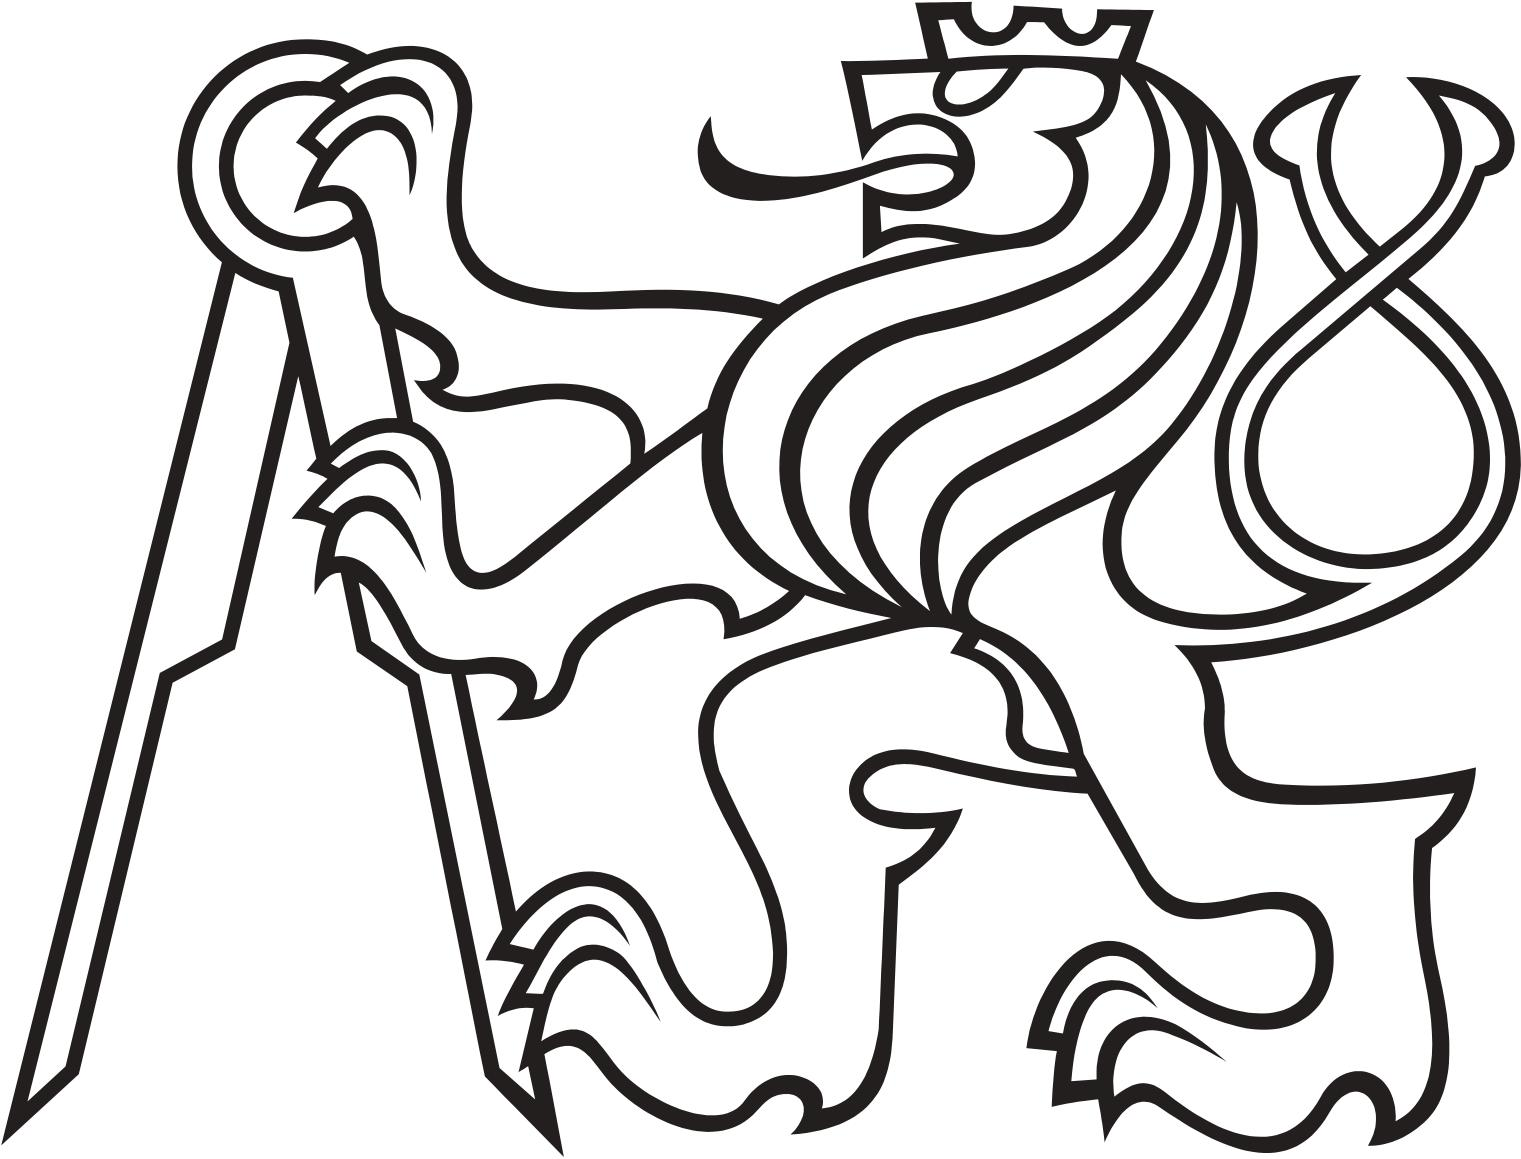
\includegraphics[width=0.3\textwidth]{ctu_logo_black.jpg}
		
		%------------------------------------------------
		%	Logo
		%------------------------------------------------
		
		\vfill\vfill
		{\large\monthyeardate\today}\\[1cm]
		
		%----------------------------------------------------------------------------------------
		
		\vfill % Push the date up 1/4 of the remaining page
		
	\end{titlepage}

	\newpage\blankpage	% a page left intentionally blank
	
	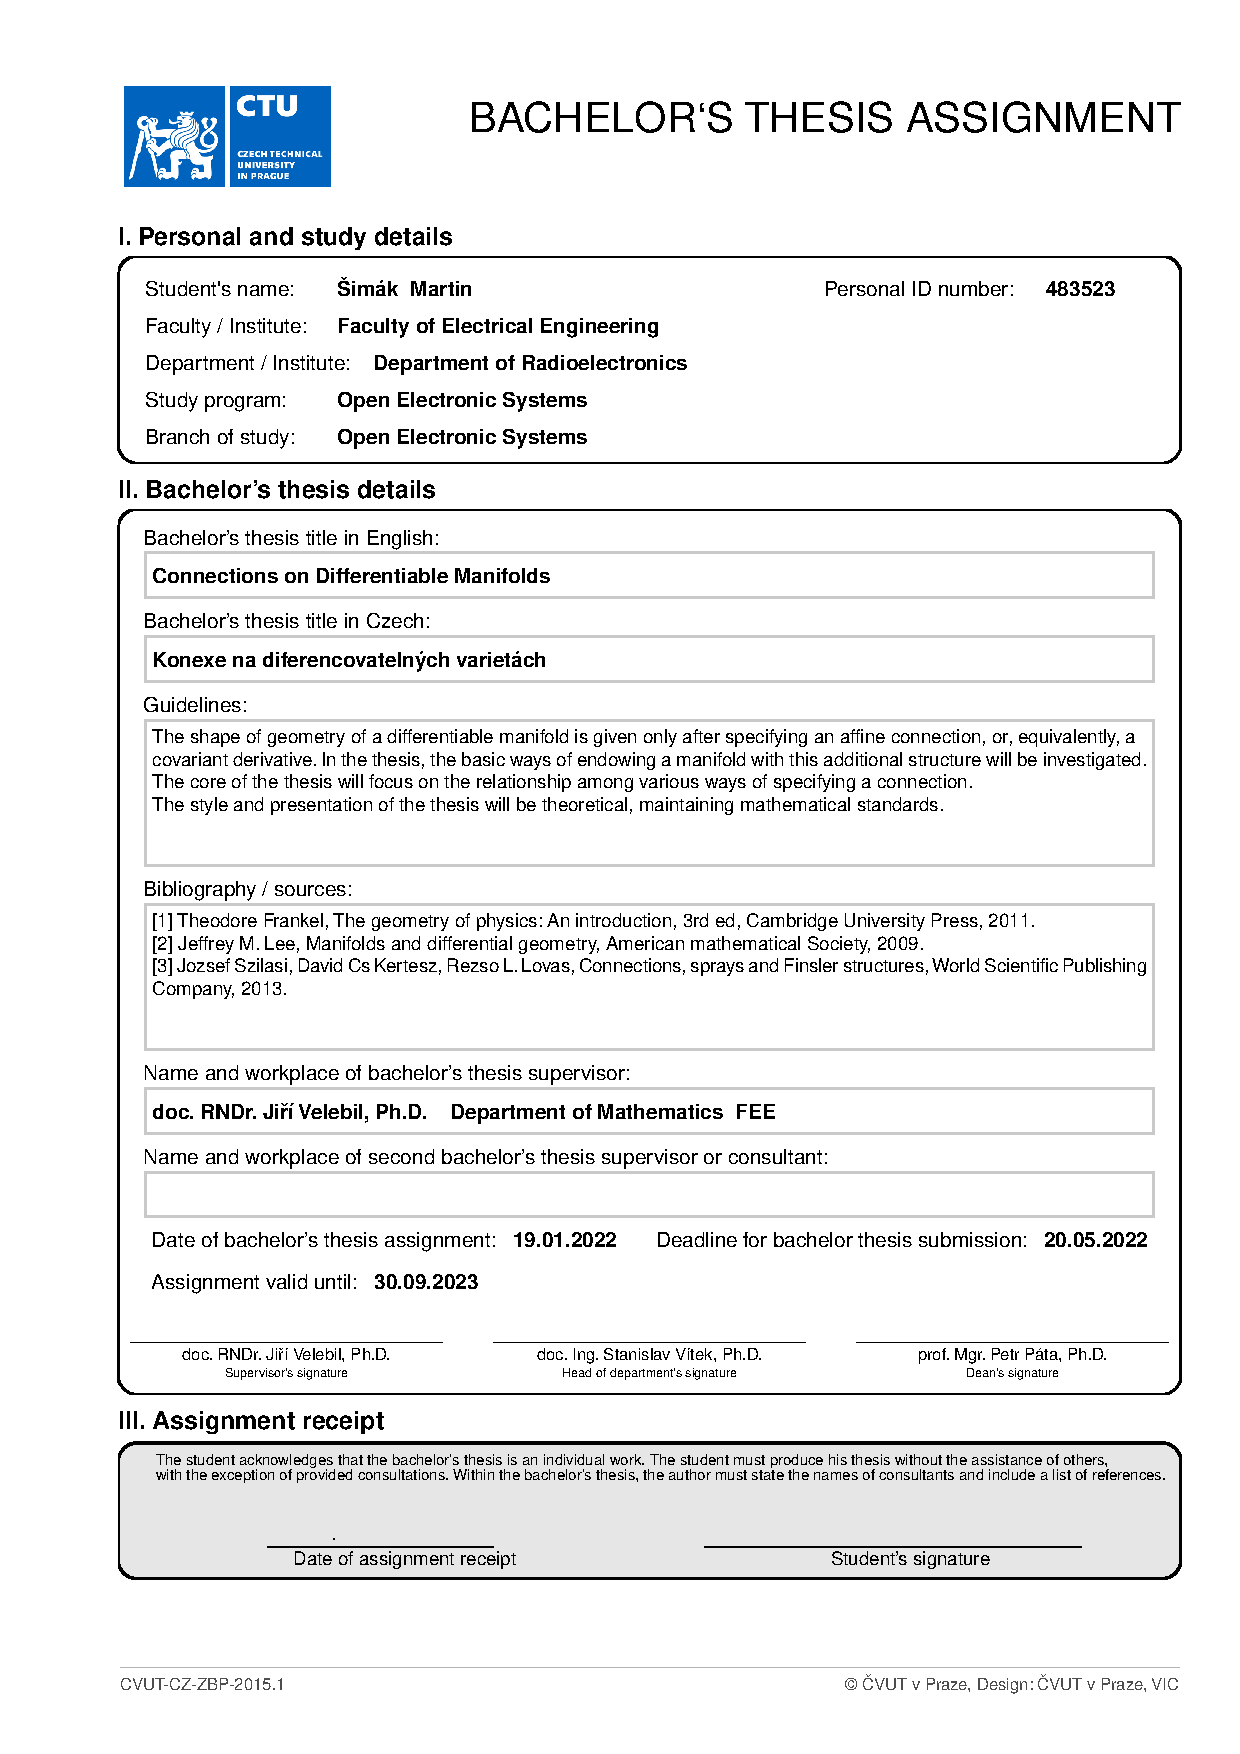
\includepdf[pages=-]{assignment.pdf}	% thesis assignment
	
	\pagenumbering{roman}
	\declarationpage	% declaration
	
	\acknowledgementspage	% acknowledge
	
	\abstractpage	% abstract
	
	\pagenumbering{arabic}
	\tableofcontents	% table of contents
	
	\chapter*{Introduction}
	\label{chap:introduction}
	\addcontentsline{toc}{chapter}{\nameref{chap:introduction}}
	
	In the year 1905, Albert Einstein published his renowned paper titled \emph{``On the Electrodynamics of Moving Bodies''} in which he reconciled \emph{Newton's laws of motion} with electrodynamics and thus laid the foundation for a whole new era in physics. In this paper---and further in the following development of the \emph{general theory of relativity} in 1915---humanity had begun to understand that our universe was not flat.
	
	One of the major discoveries Einstein's relativity brings is that spacetime has a non-trivial curvature that can be directly related to the energy and momentum of matter and radiation. This discovery naturally inspired a great number of mathematicians to find a new tool that would elegantly grasp the nature of the universe. These efforts led to a rapid development of \emph{differential geometry}. Such an outburst of interest in a fairly new branch of mathematics---the notion of a \emph{topological space} was distilled by Felix Hausdorff only in 1914---can be at least partially attributed to this phenomenal discovery.
	
	However, it is worth mentioning that although Einstein's work was definitely a massive inspiration for academic contributions in the area of calculus on curved geometries, his observation was definitely not the first. In this regard, we can mention that in the 19th century, William Kingdon Clifford in his philosophical writings coined the expression of \emph{mindstuff}, i.e., a geometry underlying the fabric of space and the curvature of which manifests itself as gravity. The rejection of a purely flat geometry reaches even further into the history as the renowned mathematician Pierre-Simon Laplace attempted to find the curvature of space already at the turn of the 19th century. Another example of earlier thoughts on the fundamental hypotheses of geometry is the classic habilitation dissertation \emph{On the hypotheses which lie at the bases of geometry} by Bernhard Riemann from 1868, translated by William Kingdon Clifford in 1873.
	
%	\vspace*{1em}
	\paragraph*{Synopsis of the thesis.} In \textbf{Chapter~\ref{chap:introduction-to-smooth-manifolds}}, we aim to explore the possible differential structure of \emph{smooth manifolds}. Although this part could be considered to be standard and left out as a pre-requisite knowledge, we prefer to inspect the introduction of the smooth manifold delicately to avoid any confusion.
	
	\textbf{Chapter~\ref{chap:tangent-spaces}} introduces a \emph{tangent structure} on a manifold. This construction allows us to locally define notions such as \emph{derivatives} and \emph{vector fields}. While all of the aforementioned should evoke an elementary course of multivariable calculus, on smooth manifolds, we will need to be more careful when defining them.
	
	Further on, in \textbf{Chapter~\ref{chap:covariant-derivatives-and-connections}}, we finally introduce the notions of a covariant derivative and a connection. In this chapter, we focus on the development of intuition on simple examples rather than a proper definition. The abstraction is instilled in \textbf{Chapter~\ref{chap:abstract-covariant-derivatives-and-abstract-connections}} where we take the conception introduced in the previous chapter and we put it into a more general setting. In this chapter, we also further explore the notions' properties and additional constructions.
	
	Ultimately, in \textbf{Chapter~\ref{chap:equivalence-of-covariant-derivative-and-connection}}, we discuss the main result of this thesis: the equivalence of a covariant derivative and a connection form. Apart from that, we also present some directions of possible generalisation of the thesis.
	
	Although the results of Chapters~\ref{chap:abstract-covariant-derivatives-and-abstract-connections} and~\ref{chap:equivalence-of-covariant-derivative-and-connection} are known, the exposition and most of the proof-work was done by me.
	
%	\begin{tcolorbox}[width=\textwidth,colback=pink,
%%			title={\bfseries{Revise}},colbacktitle=blue!20,coltitle=black,
%			boxrule=0pt]
%		Finally, the third chapter focuses on the translation of the differential calculus defined locally between tangent spaces at different points. This can be done in the language of \emph{covariant derivatives} or \emph{connections}. One of the main results of this section is the relation of these two notions to each other.
%		
%		While a considerable part of the thesis explores the studied field in a standard way, it should not be condemned as a mere compilation of several texts. Most notably in \textbf{Chapter 3}, we acquire a contemporary viewpoint called \emph{synthetic geometry} which utilises the modern \emph{category theory}. Specifically, this part has been inspired by recent academic papers and most of the proof-work has been done by me.
%	\end{tcolorbox}
		
	
	
	%---------------------------------------------------------
	%	First chap: Smooth Manifolds
	%---------------------------------------------------------
	\chapter{Introduction to smooth manifolds}
	\label{chap:introduction-to-smooth-manifolds}
	
	In the first chapter of this thesis, we introduce the concept of a smooth manifold. To readers experienced in topology, definition of the aforementioned might come across as trivial, but we consider it very important to specify how exactly we approach manifolds in general, since the underlying definitions might differ from text to text.
	
	Apart from the smooth manifold itself, we will also introduce other key concepts of differential topology, such as charts, atlases, paracompactness, etc.
	
	Our presentation of these notions follows closely the exposition given in the book~\cite{lee:manifolds-and-differential-geometry}.
	
	\section{Charts and atlases}
	
		Before we begin, let us discuss the goal of this section. We would like to introduce a structure on a set that endows it with the property of ``looking like'' $\mathbb R^n$ locally. In general, this will not be necessarily achievable globally on the whole set but we will manage to arrive at a reasonable compromise using charts and atlases.
	
		\begin{definition}
			\index{chart}
			Let $M$ be a set. A \emph{chart} on $M$ is a pair $(U,\mathbf x)$ consisting of $U \subseteq M$ and an injective map $\mathbf x:U \to \mathbb R^n$ such that $\mathbf x[U] = \{\mathbf x(a) \mid a \in U\}$ is an open set in $\mathbb R^n$. The composite $x^i = \mathrm{pr}_i \circ \mathbf x: M \to \mathbb R$ is often called the \emph{$i$-th coordinate function}.
		\end{definition}
		
		\begin{note}
			Since $\mathbf x$, by definition, has $\R^n$ as a codomain, we can always write its action upon a point $p \in M$ as $\mathbf x: p \mapsto \mathbf x(p) = \big( x^1(p),\dots,x^n(p) \big)$. Whenever we wish to emphasise the individual coordinate functions, we write $\big( x^1,\dots,x^n \big)$ or $\big( x^i \big)$ instead of $\mathbf x$.
		\end{note}
		
		\begin{remark}
			Note that we have defined charts on a plain set $M$. Therefore, we do not require $U$ in $(U,\mathbf x)$ to be open since we do not have the topological structure on $M$ just yet.
		\end{remark}
	
		\begin{definition}
			\label{def:smooth-atlas}\index{smooth atlas}
			A collection $\mathcal A \coloneqq \{(U_\alpha, \mathbf x_\alpha) \mid \alpha \in A\}$ of $\mathbb R^n$-valued charts on a given set $M$ is called a \emph{smooth} ($\mathbb R^n$-\emph{valued}) \emph{atlas} on $M$, if the following three conditions hold:
			\begin{enumerate}[label=\rm(\alph*)]
				\item $\bigcup_{\alpha \in A} U_\alpha = M$, i.e., the collection $\{U_\alpha \mid \alpha \in A\}$ covers $M$.
				\item For every $\alpha, \beta \in A$, the sets $\mathbf x_\alpha[U_\alpha \cap U_\beta] = \{\mathbf x_\alpha(a) \mid a \in U_\alpha \cap U_\beta\}$ are open in $\mathbb R^n$.
				\item Whenever $U_\alpha \cap U_\beta \neq \emptyset$, the map $\mathbf x_\beta \circ \mathbf x_\alpha^{-1}: \mathbb R^n \to \mathbb R^n$ is smooth (i.e., it has all derivatives). We also say that $(U_\alpha, \mathbf x_\alpha), (U_\beta, \mathbf x_\beta)$ are \emph{smooth-related}.
			\end{enumerate}
		\end{definition}
		
		\begin{remark}
			The above notation $\mathbf x_\beta \circ \mathbf x_\beta^{-1}$ is a shorthand for the precise, yet clumsy,
			\begin{equation*}
				\mathbf x_\beta \restr_{U_\alpha \cap U_\beta} \circ \, \mathbf x_\alpha^{-1} \restr_{\mathbf x_{\alpha}[U_\alpha \cap U_\beta]},
			\end{equation*}
			where $f \restr_A$ denotes the standard domain restriction of $f$ to $A$.
		\end{remark}
	
		\begin{definition}
			Suppose $\mathcal A_1$ and $\mathcal A_2$ are smooth $\mathbb R^n$-valued atlases on a set $M$. Define
			\begin{equation*}
				\mathcal A_1 \equiv \mathcal A_2 \quad \Longleftrightarrow \quad \text{$\mathcal A_1 \cup \mathcal A_2$ is a smooth $\mathbb R^n$-valued atlas on $M$}.
			\end{equation*}
		\end{definition}
	
		\begin{claim}
			Let $\equiv$ be the relation defined above. Then the following hold:
			\begin{enumerate}[label=\rm(\roman*)]
				\item $\equiv$ is an equivalence relation on the set of all smooth $\mathbb R^n$-valued atlases on a set $M$.
				\item Given an atlas $\mathcal A$, the union $\bigcup \{\mathcal B \mid \mathcal B \equiv \mathcal A\}$ is an atlas again. Moreover, this atlas is equivalent to $\mathcal A$. Let us call it the \emph{maximal atlas} generated by $\mathcal A$ and denote it $\mathcal A^{\mathrm{max}}$.
				\item Let $[\mathcal A]_\equiv = \{\mathcal B \mid \mathcal B \equiv \mathcal A\}$ be the equivalence class of an atlas $\mathcal A$ under the relation $\equiv$. The correspondence $[\mathcal A]_\equiv \mapsto \mathcal A^{\mathrm{max}}$ is a bijection.
			\end{enumerate}
		\end{claim}
		
		\begin{proof}
			Ad (i): For a relation to be an equivalence, it must hold that the relation is reflexive, symmetric and transitive.
			\begin{enumerate}[label=\rm(\alph*)]
				\item For reflexivity, we need to show that $\mathcal A \equiv \mathcal A$. This fact is trivial, since $\mathcal A$ is a smooth atlas and $\mathcal A \cup \mathcal A = \mathcal A$ holds, thus $\mathcal A \equiv \mathcal A$ is obvious.
				\item Symmetry means that $\mathcal A_1 \equiv \mathcal A_2$ if and only if $\mathcal A_2 \equiv \mathcal A_1$. This follows naturally from the symmetry of the relation $\cup$.
				\item Transitivity: if $\mathcal A_1 \equiv \mathcal A_2$ and $\mathcal A_2 \equiv \mathcal A_3$, then $\mathcal A_1 \equiv \mathcal A_3$. This fact is easily checked by going through the defining properties.
			\end{enumerate}
		
			Ad (ii): First, we should note that $\mathcal A^{\mathrm{max}}$ surely is an atlas in the first place. This is trivially guaranteed by the fact that $\mathcal A^{\mathrm{max}}$ is a union of elements that are already atlases themselves. Next, let us verify that $\mathcal A^{\mathrm{max}}$ is equivalent to $\mathcal A$. Thanks to the reflexivity of $\equiv$, it holds that $\mathcal A \subseteq \mathcal A^{\mathrm{max}}$, i.e., $\mathcal A \cup \mathcal A^{\mathrm{max}} = \mathcal A^{\mathrm{max}}$, which is an atlas based on the preceding discussion.
			
			Ad (iii): The bijective correspondence follows easily from the fact that both $[\mathcal A]_\equiv$ and $\mathcal A^{\mathrm{max}}$ are defined by collecting atlases equivalent to $\mathcal A$ and their unions, respectively.
		\end{proof}
	
		\begin{definition}
			Let $(U, \mathbf x)$ be a chart on $M$ and let $\mathcal A$ be a smooth atlas on $M$. We say that $(U, \mathbf x)$ is \emph{compatible} with $\mathcal A$, provided that $\mathcal A \cup \{(U, \mathbf x)\}$ is an atlas on $M$.
		\end{definition}
	
		\begin{claim}
			\label{claim:compatible-charts}
			Let $\mathcal A = \{(U_\alpha, \mathbf x_\alpha) \mid \alpha \in A\}$ be a smooth $\mathbb R^n$-valued atlas on a set $M$. Then the following holds:
			\begin{enumerate}[label=\rm(\roman*)]
				\item Let $(U,\mathbf x)$ and $(V, \mathbf y)$ are charts compatible with $\mathcal A$, and such that $U \cap V \neq \emptyset$. Then the charts $(U \cap V, \mathbf x \restr_{U \cap V})$ and $(U \cap V, \mathbf y \restr_{U \cap V})$ are compatible with $\mathcal A$, hence they both belong to the maximal atlas generated by $\mathcal A$.
				
				\item Let $(U, \mathbf x)$ be a chart compatible with $\mathcal A$, let $O$ be an open subset of $\mathbf x[U]$ and let $V$ denote $\mathbf x^{-1}[O]$. Then $(V,\mathbf x \restr_V)$ is a chart compatible with $\mathcal A$.
			\end{enumerate}
		\end{claim}
	
		\begin{proof}
			\begin{enumerate}[label=\rm(\roman*)]
				\item For $(U \cap V, \mathbf x \restr_{U \cap V})$ to be compatible with $\mathcal A$, it must hold that $\mathcal A \cup \{(U \cap V, \mathbf x \restr_{U \cap V})\}$ is an atlas over $M$, i.e., that it satisfies the conditions (a)---(c) in Definition~\ref{def:smooth-atlas}.
				\begin{enumerate}[label=\rm(\alph*)]
					\item The collection $\{U_\alpha \mid \alpha \in A\} \cup \{U \cap V\}$ obviously covers $M$.
					\item For every $\alpha \in A$, it holds that the sets $\mathbf x_\alpha[U_\alpha \cap U]$ and $\mathbf x_\alpha[U_\alpha \cap V]$ are open in $\R^n$. Further, since
					\begin{align*}
						\mathbf x_\alpha[U_\alpha \cap U \cap V] = \mathbf x_\alpha[U_\alpha \cap U] \cap \mathbf x_\alpha[U_\alpha \cap V]
					\end{align*}
					holds and since finite intersections of open sets are open, we immediately obtain that $\mathbf x_\alpha[U_\alpha \cap U \cap V]$ is open in $\R^n$, for every $\alpha \in A$. Hence, the chart $(U \cap V, \mathbf x\restr_{U \cap V})$ is compatible with $\mathcal A$.
					
					\item Whenever $U_\alpha \cap U \cap V \neq \emptyset$, the maps $\mathbf x \restr_{U \cap V} \circ \, \mathbf x_\alpha^{-1}$ and $\mathbf x_\alpha \circ \mathbf x \restr_{U \cap V}^{-1}$ are smooth. This condition holds trivially, since both restrictions and compositions of smooth maps are also smooth.
				\end{enumerate}
				Since for $(U \cap V, \mathbf y \restr_{U \cap V})$, the reasoning is analogous, we consider this proved.
				
				\item For the second part, we construct a very similar proof to the above. Let us show that $\mathcal A \cup \{(V, \mathbf x \restr_V)\}$ is an atlas:
				\begin{enumerate}[label=\rm(\alph*)]
					\item The collection $\{U_\alpha \mid \alpha \in A\} \cup \{V\}$ covers $M$ for obvious reasons.
					\item For each $\alpha \in A$, the sets $\mathbf x_\alpha[U_\alpha \cap V]$ and $\mathbf x \restr_V[U_\alpha \cap V]$ are open in $\mathbb R^n$ due to the fact that $(U, \mathbf x)$ is compatible with $\mathcal A$ and that $V$ is the inverse image of an open set in $\mathbb R^n$ under $\mathbf x$.
					\item Whenever $U_\alpha \cap V \neq \emptyset$, the maps $\mathbf x\restr_V \circ \, \mathbf x_\alpha^{-1}$ and $\mathbf x_\alpha \circ \mathbf x\restr_V^{-1}$ are smooth because we are once again dealing with restrictions and compositions of smooth maps.
				\end{enumerate}
			\end{enumerate}
		\end{proof}
	
	
	\section{Topology}
	
		Now, let us turn our focus to topology. To introduce our desired construction---a smooth manifold---we will have to review some of the basic definitions such as the topology and open sets, basis, etc. Apart from these elementary notions, we will also demand that our smooth manifold is also Hausdorff and paracompact which are delicate properties we will talk about later. An excellent survey of general topology is the book~\cite{engelking:general-topology}.
		\begin{definition}
			\index{topology}\label{def:topology}
			Let $X$ be a set and let $\tau$ be a family of subsets of $X$ such that the following conditions hold:
			\begin{enumerate}[label=\rm(\alph*)]
				\item $\emptyset \in \tau$ and $X \in \tau$.
				\item If $U_1 \in \tau, \dots, U_n \in \tau$, then $U_1 \cap \dots \cap U_n \in \tau$.
				\item If $U_i \in \tau$, $i \in I$, then $\bigcup_{i \in I} U_i \in \tau$.
			\end{enumerate}
			Such family $\tau$ is called \emph{topology}, elements of $\tau$ are called \emph{open sets} and we say that the pair $(X,\tau)$ forms a \emph{topological space}.
		\end{definition}
		
		\begin{remark}
			The notion of a topological space is a vast generalisation of the familiar notion of a metric space.
			
			More in detail: any metric space $(X,d)$ becomes a topological space $(X,\tau_d)$ by declaring $U \subseteq X$ to be in $\tau_d$ (i.e., declaring $U$ to be open in $(X,\tau_d)$) whenever the following holds:
			\begin{itemize}
				\item[] given $p \in U$, there exists $r > 0$ such that $B_r(p) = \{x \in X \mid d(p,x) < r\} \subseteq U$.
			\end{itemize}
			Then it is easy to prove that $\tau_d$ is indeed a topology on $X$.
			
			Hence, the notion of a topological space axiomatises the well-known property of open sets in a metric space: an open set is a set, where one can ``wiggle around'' any of the points a bit without leaving the open set.
			
			Of course, we cannot talk about any notion of distance in a general topological space. In fact, it is easy to come up with an example of a topological space $(X,\tau)$ such that $\tau \neq \tau_d$ for any metric $d$ on $X$. Consider, for example, $X=\{a,b\}$ and $\tau=\{\emptyset,X\}$.
		\end{remark}
	
		\begin{definition}
			\label{def:basis}
			A collection $\mathcal B$ of subsets of a set $X$ is called the \emph{basis}, if the following hold:
			\begin{enumerate}[label=\rm(\alph*)]
				\item $\mathcal B$ covers $X$, i.e., $\bigcup_{B \in \mathcal B} B = X$.
				\item If $B_1 \in \mathcal B$, $B_2 \in \mathcal B$ and $x \in B_1 \cap B_2$, then there exists a basis element $B \in \mathcal B$ such that $x \in B \subseteq B_1 \cap B_2$.
			\end{enumerate}
		\end{definition}
	
		\begin{claim}
			\label{claim:topology-generated-by-basis}
			Let $\mathcal B$ be a basis of subsets of $X$. Then the collection $\tau$ of arbitrary unions of elements of $\mathcal B$ forms a topology on $X$. This topology is called the topology \emph{generated} by $\mathcal B$.
		\end{claim}
	
		\begin{proof}
			Using the defining properties of a basis, we shall verify that the conditions (a)--(c) of Definition~\ref{def:topology} indeed hold when taking unions of the elements of $\mathcal B$.
			\begin{enumerate}[label=\rm(\alph*)]
				\item Both $\emptyset$ and all of $X$ can be formed as specific unions of elements of $\mathcal B$. The former can be constructed as a union of zero elements and the latter by taking the union of all elements of $\mathcal B$ which makes up the whole of $X$, thanks to (a) in Definition~\ref{def:basis}.
				\item Any arbitrary finite intersection can be constructed by repeated application of the second property of basis elements.
				\item This condition holds trivially as we take all possible unions into account.
			\end{enumerate}
		\end{proof}
	
		\begin{claim}
			\label{claim:topology-generated-by-atlas}
			If $\mathcal A = \{(U_\alpha, \mathbf x_\alpha) \mid \alpha \in A\}$ is a maximal smooth atlas on $M$, then the collection $\{U_\alpha \mid \alpha \in A\}$ is a basis for a topology on $M$ (called the \emph{topology induced by} $\mathcal A$).
		\end{claim}
	
		\begin{proof}
			First, we will show that $\{U_\alpha \mid \alpha \in A\}$ forms a basis on $M$. The first condition of covering $M$ holds immediately when reviewing the definition of an atlas. The second condition is assured by Claim~\ref{claim:compatible-charts}. Now that have a basis on $M$, we can generate a topology on $M$ by taking arbitrary unions of elements of the basis as we have seen in Claim~\ref{claim:topology-generated-by-basis}.
		\end{proof}
	
		\begin{claim}
			Let $M$ be a set equipped with a maximal atlas $\mathcal A = \{(U_\alpha, \mathbf x_\alpha) \mid \alpha \in A\}$ and a topology $\tau$ induced by $\mathcal A$. This topology can be characterised as follows: $V \subseteq M$ is open if and only if $\mathbf x_\alpha[U_\alpha \cap V]$ is an open subset of $\mathbb R^n$ for all charts $(U_\alpha, \mathbf x_\alpha)$ of $\mathcal A$.
		\end{claim}
	
		\begin{proof}
			To prove the logical equivalence used in the body of the claim, we shall break it down into two implications:
			\begin{itemize}
				\item "$\implies$": Let $V \subseteq M$ be an open set within the topology $\tau$. Following Claim~\ref{claim:topology-generated-by-atlas}, it can be written as $V = \bigcup_{\alpha \in I} U_\alpha$ for some $(U_\alpha,\mathbf x_\alpha)$ in $\mathcal A$. Therefore $\mathbf x_\alpha [U_\alpha \cap V]$ is indeed an open subset of $\mathbb R^n$ for every $\alpha \in A$ from the definition of an atlas.
				
				\item "$\impliedby$": Let $\mathbf x_\alpha[U_\alpha \cap V]$ be an open subset of $\mathbb R^n$ for all charts $(U_\alpha, \mathbf x_\alpha)$ of $\mathcal A$. This implication is a simple consequence of what we have seen in Claim~\ref{claim:compatible-charts}. For every $O_\alpha = \mathbf x_\alpha[U_\alpha \cap V]$, we get an inverse image $V_\alpha = \mathbf x_\alpha^{-1}[O_\alpha]$, which, according to the referred claim, is a chart when accompanied by the restriction $\mathbf x_\alpha \restr_{V_\alpha}$ and thus belongs to the maximal atlas. If we do this to all the intersections in $\mathbb R^n$, we get a collection of open sets in $M$ under the topology $\tau$, which was generated by the atlas $\mathcal A$. However, the topology $\tau$ was naturally created by taking arbitrary unions of elements of $\{ U_\alpha \mid \alpha \in A \}$. This indeed means that $V$ as a union of $V_\alpha$ belongs to $\tau$ as well and therefore is an open set.
			\end{itemize}
		\end{proof}
	
		As we said at the beginning, a manifold should locally ``look like'' $\R^n$. Now we have the tools to say it precisely.
		\begin{definition}
			A topological space $(X,\tau)$ is called \emph{locally Euclidean} if each point $x \in X$ has an open neighbourhood that is homeomorphic to an open subset of $\mathbb R^n$.
		\end{definition}
		
		\begin{note}
			The above definition of a locally Euclidean space assumes the definition of a homeomorphism as a mapping $f:X \to Y$ between two topological spaces $(X,\tau)$ and $(Y,\sigma)$, which is bijective and continuous both ways, i.e., both $f$ and $f^{-1}$ are continuous. In topology, continuous maps ``reflect'' openness, i.e., if $V \subseteq Y$ is an open set under the topology $\sigma$ on $Y$, then the inverse image $f^{-1}(V) \subseteq X$ is an open set under the topology $\tau$ on $X$.
		\end{note}
		
		\begin{remark}
			\label{remark:locally-euclidean-not-hausdorff}
			The definition of a smooth manifold that we are heading towards should formalise the notion of a topological space which locally ``looks like'' $\mathbb R^n$. There are spaces, however, that locally ``look like'' $\mathbb R^n$, yet they do not have an important property of a Euclidean space.
			
			Consider the space $X = (\mathbb R \times \{0\}) \cup (\mathbb R \times \{1\})$ with the topology $\tau$ of a subspace of $\mathbb R^2$ (the space $(X,\tau)$ consists of two parallel lines in the plane). Now define an equivalence relation $\sim$ on $X$ by putting $(x,0) \sim (x,1)$ for all $x \in \mathbb R \setminus \{0\}$.
			
			If we endow the quotient set $X/_\sim$ with the quotient topology%
			\footnote{Since the notion of a quotient topology serves as a mere example in this thesis, we do not elaborate on it any further. For more information about quotient topologies, see e.g.,~\cite{engelking:general-topology}.}
			$\tau_\sim$ (i.e., declare $U \subseteq X/_\sim$ open, whenever $\pi^{-1}(U)$ is open in $X$, where $\pi: X \to X/_\sim$ is the quotient map), then the space $(X/_\sim, \tau_\sim)$ is not convenient for us since e.g., the points $[(0,0)]_\sim$ and $[(0,1)]_\sim$ cannot be distinguished in $(X/_\sim,\tau_\sim)$ by disjoint open sets, yet every point of $X/_\sim$ has an open neighbourhood that is homeomorphic to $\mathbb R$.
		\end{remark}
		
		Thus, the space $(X/_\sim,\tau_\sim)$ from the above remark lacks the property that any pair of its distinct points can be ``separated'' by two disjoint open sets. In a slogan, such a property means that any two distinct points are ``quite far away''. We formulate the property precisely now.
		\begin{definition}
			A topological space $(X, \tau)$ is called \emph{Hausdorff} (also that it \emph{satisfies the $T_2$ axiom}), if for all $x \neq y$ in $X$ there exist disjoint open sets $U$, $V$ such that $x \in U$ and $y \in V$.
		\end{definition}
	
		Thus, Remark~\ref{remark:locally-euclidean-not-hausdorff} gives an example of a locally Euclidean space that is not Hausdorff. It is quite easy to see why such property is convenient for us. For a topological space to be Hausdorff it simply means that we can make a clear distinction (via separation by open neighbourhoods) between two different points of that space. This proves especially convenient when treating further notions such as unambiguity of a limit.
		
		There are two other desirable properties a manifold should have: it should be second countable and/or paracompact. Let us mention that these additional properties are there for comfort only: non-paracompact manifolds are studied as well, see~\cite{gauld:nonmetrisable-manifolds}.
		\begin{definition}
			A topological space $(X, \tau)$ is called \emph{second countable}, if $\tau$ has an at most countable basis.
		\end{definition}

		\begin{definition}
			Let $(X,\tau)$ be a topological space.
			\begin{itemize}
				\item A collection $\{U_i \mid i \in I\}$ is an \emph{open cover} of $X$, if $\bigcup_{i \in I} U_i = X$ and every $U_i$ is an open set.
				\item An open cover $\{V_j \mid j \in J\}$ is a \emph{refinement} of an open cover $\{U_i \mid i \in I\}$, if for every $j \in J$ there exists an $i \in I$ such that $V_j \subseteq U_i$.
				\item A cover $\{U_i \mid i \in I\}$ is called \emph{locally finite}, provided that for every $x \in X$, there exists an open set $U$ such that $x \in U$ and the set $\{i \in I \mid U \cap U_i \neq \emptyset\}$ is finite.
			\end{itemize}
		\end{definition}

		\begin{definition}
			\index{paracompactness}
			A topological space $(X, \tau)$ is called \emph{paracompact}, if the following holds: every open cover of $X$ has a locally finite refinement to an open cover.
		\end{definition}
		
		Roughly speaking: paracompactness of a manifold ensures that one can perform certain constructions locally and then ``glue'' them together in a non-conflicting, pleasing way. This is particularly useful when defining, e.g., \emph{integration} on a manifold. We do not develop integral calculus in this text. For details, see, e.g.,~\cite{lee:manifolds-and-differential-geometry}.
		
		The following result shows why second countability and paracompactness are also topologically desirable. We state the theorem without proof. For details, we refer to~\cite{engelking:general-topology}.
		\begin{theorem}
			Suppose $(X,\tau)$ is a Hausdorff, locally Euclidean space. Then the following conditions are equivalent:
			\begin{enumerate}[label=\rm(\roman*)]
				\item $(X,\tau)$ is paracompact.
				\item $(X,\tau)$ is a metrisable space.
				\item Each connected component of $(X,\tau)$ is second countable.
				\item Each connected component of $(X,\tau)$ is $\sigma$-compact (i.e., it is a union of at most countably many compact spaces).
				\item Each connected component of $(X,\tau)$ is separable (i.e., it contains an at most countable dense subset).
			\end{enumerate}
		\end{theorem}
		
		As the final step towards our definition of a smooth manifold, we formulate the following claim which shows how to attain the ``nice'' properties we have defined earlier (being Hausdorff, second countable and paracompact) via specific requirements on our smooth structure.
		\begin{claim}
			\label{claim:classification-of-hausdorff-paracompact-secound-countable}
			Let $\mathcal A$ be a smooth atlas on a set $M$. Then the following holds:
			\begin{enumerate}[label=\rm(\roman*)]
				\item Suppose that, for any $p \neq q$ in $M$, we have either charts $(U_\alpha, \mathbf x_\alpha)$, $(U_\beta, \mathbf x_\beta)$ with $U_\alpha \cap U_\beta = \emptyset$ and $p \in U_\alpha$, $q \in U_\beta$, or there exists a chart $(U,\mathbf x)$ such that $p \in U$ and $q \in U$. Then the topology on $M$ given by $\mathcal A$ is Hausdorff.
				\item If $\mathcal A$ is countable (or if it has a countable subatlas), then the topology $\tau$ on $M$ induced by $\mathcal A$ is second countable.
				\item If the collection $\{U_\alpha \mid \alpha \in A\}$ of chart domains of $\mathcal A$ is such that for every $\alpha_0 \in A$, the set $\{ \alpha \in A \mid U_\alpha \cap U_{\alpha_0} \neq \emptyset\}$ is at most countable, then the topology on $M$ induced by $\mathcal A$ is paracompact.
			\end{enumerate}
		\end{claim}
	
		\begin{proof}
			\begin{enumerate}[label=\rm(\roman*)]
				\item Since the first condition indirectly copies the definition of a Hausdorff space, we will only tend to the latter one. If there exists a chart $(U,\mathbf x)$ such that both $p$ and $q$ belong to $U$, then due to the injectivity of $\mathbf x$, we obtain $\mathbf x(p) \neq \mathbf x(q)$. Since $\R^n$ is a Hausdorff space, we can separate by open sets: $\mathbf x(p) \in U_p$ and $\mathbf x(q) \in U_q$, where $U_p \cap U_q = \emptyset$ and both $U_p$ and $U_q$ are open. According to Claim~\ref{claim:compatible-charts}, we can then follow the inverse images $\mathbf x^{-1}[U_p]$ and $\mathbf x^{-1}[U_q]$ and consider them open since they form compatible chart domains. Once again, thanks to the injectivity of $\mathbf x$, we have two disjoint open sets separating $p$ and $q$.
				
				\item This claim is trivial since the topology $\tau$ is generated by taking arbitrary unions of chart domains from $\mathcal A$. Therefore the set $\tau$ contains a countable amount of basis elements.
				
				\item We refer to~\cite{lee:manifolds-and-differential-geometry} for the full (rather technical) proof.
			\end{enumerate}
		\end{proof}
	
		Now, we arrive at the point where we know what all of our desirable properties really mean and we are ready to define the final concept of this chapter---the definition of a smooth manifold.
		\begin{definition}
			\index{smooth manifold}
			An \emph{$n$-dimensional smooth manifold} is a pair $(M, \mathcal A)$, where $M$ is a set and $\mathcal A$ is a smooth ($\R^n$-valued) atlas on $M$, such that the topology on $M$ induced by $\mathcal A$ is Hausdorff and paracompact.
		\end{definition}
	
		\begin{note}
			An $n$-dimensional smooth manifold is often referred to as a smooth $n$-manifold. It is also common to call just the set $M$ a manifold when specification of the atlas is unnecessary for the sake of brevity.
		\end{note}
		
		\begin{definition}
			\index{smooth map}
			Let $M$ and $N$ be smooth manifolds, and let $F: M \to N$ be a map. We say that $F$ is 
			\emph{smooth} if for every $p \in M$ there exist smooth charts $(U,\mathbf x)$ containing $p$ and $(V,\mathbf y)$ containing $F(p)$ such that $F[U] \subseteq V$ and the composite $\mathbf y \circ F \circ \mathbf x^{-1}: \mathbf x[U] \to \mathbf y[V]$ is smooth.
		\end{definition}
	
		\begin{notation}
			In the following, we will often use the symbol $C^\infty(M)$ to denote the set of all smooth, real-valued maps on $M$.
		\end{notation}
	
	\section{Examples of smooth manifolds}
	
		Before we proceed to further explore the general theory of smooth structures on manifolds, let us show some examples of what we can classify as a smooth manifold.
		\begin{example}[Euclidean Spaces]
			For every $n \in \N_0$, the Euclidean space $\R^n$ is a smooth manifold $(\R^n,\{(\R^n,\id_{\R^n})\})$ of dimension $n$. Notice that this smooth structure is not canonically given and is called the \emph{standard smooth structure on} $\R^n$.
		\end{example}
	
		\begin{example}[Spheres in Euclidean spaces]
			\index{sphere}\label{ex:n-sphere}
			Let $\norm{-}$ be the Euclidean norm on $\R^{n+1}$, $n \geq 0$. The unit sphere
			\begin{align*}
				\mathbb S^n \coloneqq \left\{ x \in \R^{n+1} \mid \norm{x} = 1 \right\}
			\end{align*}
			is indeed Hausdorff and second-countable as it is a topological subspace of $\R^{n+1}$. To inspect its structure, let us denote for each $i \in \{1, \dots, n+1 \}$
			\begin{align*}
				U_i^+ &\coloneqq \left\{ \(x^1,\dots,x^{n+1}\) \in \R^{n+1} \mid x^i > 0 \right\},
			\\
				U_i^- &\coloneqq \left\{ \(x^1,\dots,x^{n+1}\) \in \R^{n+1} \mid x^i < 0 \right\}.
			\end{align*}
			Now consider the continuous function $f:\mathbb B^n \to \R$
			\begin{align*}
				f(u) &= \sqrt{1-\norm u^2},
			\end{align*}
			where $\mathbb B^n = \{ x \in \R^n \mid \norm x < 1 \}$. Now it is easy to see that $U_i^+ \cap \mathbb S^n$ and $U_i^- \cap \mathbb S^n$ are the graphs of functions
			\begin{align*}
				x^i &= f\(x^1,\dots,x^{i-1},x^{i+1},\dots,x^{n+1}\),
			\\
				x^i &= -f\(x^1,\dots,x^{i-1},x^{i+1},\dots,x^{n+1}\)
			\end{align*}
			respectively. Therefore, we can conclude that each subset $U_i^{\pm} \cap \mathbb S^n$ is locally Euclidean of dimension $n$ and that the maps $\mathbf x_i^{\pm}: U_i^\pm \cap \mathbb S^n \to \mathbb B^n$ given by
			\begin{align*}
				\mathbf x_i^\pm\(x^1,\dots,x^{n+1}\) = \(x^1,\dots,x^{i-1},x^{i+1},\dots,x^{n+1}\)
			\end{align*}
			are graph coordinates for $\mathbb S^n$. Now let us take an arbitrary composition $\mathbf x_i^\pm \circ \big(\mathbf x_j^\pm\big)^{-1}$, where we can assume that $i<j$. Explicitly, we obtain
			\begin{align*}
				\mathbf x_i^\pm \circ \big(\mathbf x_j^\pm\big)^{-1}\(x^1,\dots,x^n\) = \( x^1,\dots, x^{i-1},x^{i+1},\dots,x^{j-1},\pm\sqrt{1-\norm x^2},x^{j+1},\dots,x^n \).
			\end{align*}
			In the case of $i>j$, we obtain a similar relation. Also, consider that if $i=j$, we get
			\begin{align*}
				\mathbf x_i^+ \circ \big(\mathbf x_i^-\big)^{-1} = \mathbf x_i^- \circ \big(\mathbf x_i^+\big)^{-1} = \id_{\mathbb B^n}.
			\end{align*}
			As we can see, the collection $\left\{ \(U_i^\pm \cap S^n, \mathbf x_i^\pm\) \right\}$ forms a smooth atlas on $\mathbb S^n$, turning it into a smooth manifold of dimension $n$.
		\end{example}
		
		\begin{remark}
			Example~\ref{ex:n-sphere} shows that one can define manifolds in $\R^{n+1}$ by using certain functions. Namely, we have used the function
			\begin{align*}
				\norm{-}: \R^{n+1} \to \R
			\end{align*}
			to conclude that the inverse image
			\begin{align*}
				\norm{-}^{-1}(1) = \{ x \in \R^{n+1} \mid \norm x = 1 \}
			\end{align*}
			is a manifold.
			
			This is an instance of a general procedure that is supported by the so-called \emph{Regular Value Theorem}. We state the theorem later, see~\ref{thm:regular-value-theorem} below.
		\end{remark}
	
	
	\chapter{Tangent spaces}
	\label{chap:tangent-spaces}
	In this chapter, we solidify the terminology and definitions of core concepts of the differential structure on manifolds such as the derivative at a point and the derivative of a smooth map between two manifolds.
	
	Thus, in Section~\ref{sec:tangent-vectors-at-a-point}, we introduce the concept of a tangent vector at a point of a manifold. We also show that these vectors quite naturally form a vector space of the same dimension as the ambient manifold. Moreover, smooth maps are able to carry tangent vectors to tangent vectors by means of a derivative of a smooth map.
	
	The point of view that derivatives of smooth maps are linear maps is central to modern differential geometry. In addition, it leads quite naturally to the concept of a tangent bundle of a manifold, i.e., of tangent spaces ``glued together'', see Section~\ref{sec:tangent-bundles}. The tangent bundle of a manifold is crucial in an easy treatment of vector fields, curves, and, ultimately, covariant derivatives.
	
	While we postpone the notion of a covariant derivative to Chapter~\ref{chap:covariant-derivatives-and-connections}, we also introduce vector fields, curves and their velocities in Sections~\ref{sec:curves-and-velocity-vectors} and~\ref{sec:vector-fields}.
	
	For further details on the material of this chapter, we refer to~\cite{lee:manifolds-and-differential-geometry} again.
	
	\section{Tangent vectors at a point}
	\label{sec:tangent-vectors-at-a-point}
	
		We would like to build a notion similar to the definition of a directional derivative in $\R^n$. We will see that such a concept will lead quite naturally to the concept of a tangent vector. Let us see an example of what we mean by that.
		
		\begin{example}
			\label{ex:tangent-vectors-at-a-point-introduction}
			Let us fix a point $p$ in the Euclidean plane $\R^2$. ``Standing'' at $p$, there are various directions, in which we can ``look''. Any such direction can be visualised as a non-zero vector $v_p = (v^1, v^2)^T$ having its foot at $p$.
			
			If a smooth function, say $f: \R^2 \to \R$, is given, we can compute the derivative of $f$ at $p$ in direction $v$ by computing the expression
			\begin{align*}
				\pder fx(p) \cdot v^1 + \pder fy(p) \cdot v^2.
			\end{align*}
			If we denote the above expression by $v_p(f)$, then it is easy to see that the assignment $f \mapsto v_p(f)$ yields a function that
			\begin{enumerate}[label=\rm(\alph*)]
				\item is linear, i.e., the equality
				\begin{align*}
					v_p(af+bg) = av_p(f) + bv_p(g)
				\end{align*}
				holds for all $a,b \in \R$ and all smooth functions $f: \R^2 \to \R$, $g: \R^2 \to \R$.
				
				\item satisfies the so-called \emph{Leibniz rule}
				\begin{align*}
					v_p(fg) = g(p) v_p(f) + f(p) v_p(g)
				\end{align*}
				for all smooth functions $f,g$.
			\end{enumerate}
		
			Conversely, if an assignment $f \mapsto v_p(f)$ satisfies conditions (a) and (b) for all smooth maps $f$, it is easy to extract a vector $(v^1,v^2)^T$ by putting
			\begin{align*}
				v^1 &= v_p(f) \quad \text{for } f(x,y) = x,
			\\
				v^2 &= v_p(g) \quad \text{for } g(x,y) = y.
			\end{align*}
			Hence, the vector $v_p$ can be identified with a map $f \mapsto v_p(f)$ satisfying (a) and (b) above.
		\end{example}
		
		The above example serves as a motivation for the following definition: we define a tangent vector at a point to be a ``derivative''.
		
		\begin{definition}
			\index{derivation at a point}\index{tangent space}
			Let $M$ be a smooth manifold of dimension $n$ and let $p \in M$. A linear map $v_p: C^\infty(M) \to \R$ is called a \emph{derivation at $p$}, if it satisfies the so-called \emph{Leibniz rule} (or, \emph{product rule})
			\begin{align*}
				v_p(fg) &= g(p) v_p(f) + f(p) v_p(g) \quad \text{for all $f,g \in C^{\infty}(M)$.}	
			\end{align*}
			The set of all derivations at $p$ is called a \emph{tangent space at $p$} and is denoted by $T_p M$.
		\end{definition}
	
		\begin{remark}
			\label{remark:tpm-is-a-linear-space}
			At any point $p \in M$, the tangent space $T_pM$ is a vector space over $\R$ with the operations $+$ and $\cdot$ defined pointwise, i.e., for $v_p,w_p \in T_p M$ and $a \in \R$:
			\begin{align*}
				(v_p+w_p)(f) &= v_p(f) + w_p(f),
			&
				(av_p)(f) &= av_p(f).
			\end{align*}
		\end{remark}
		
		\begin{example}
			\label{ex:partial-derivatives-intro}
			An important example of a derivation at a point is the ``partial'' derivative with respect to a chart. More in detail, given a chart $(U,\mathbf x)$ of an $n$-dimensional manifold $M$ and a point $p \in U$, we define
			\begin{align*}
				\left.\frac{\p}{\p x^i}\right|_p : C^\infty(M) \to \R
			\end{align*}
			as follows:
			\begin{align*}
				\left.\frac{\p}{\p x^i}\right|_p (f) = \p_i\(f \circ \mathbf x^{-1}\)(\mathbf x(p)).
			\end{align*}
			Above, on the right-hand side, we have used $\p_i$ to denote the usual partial derivative with respect to the $i$-th coordinate of the function $f \circ \mathbf x^{-1}: \mathbf x[U] \to \R$. It is then easy to show that $\p/\p x^i|_p$ is indeed a derivation at $p$. Notice that the above is chart-dependent and we should have written the more precise
			\begin{align*}
				\left.\frac{\p}{\p x^i}\right|_{(U,\mathbf x),p}.
			\end{align*}
		\end{example}
		
		\begin{lemma}
			\label{lemma:derivatives-properties}
			Let $M$ be a smooth manifold, let $p \in M$, $v_p \in T_pM$, and $f$, $g \in C^\infty$. Then the following hold:
			\begin{enumerate}[label=\rm(\roman*)]
				\item If $f$ is a constant function, then $v_p(f)=0$.
				\item If $f(p) = g(p) = 0$, then $v_p(fg) = 0$.
			\end{enumerate}
		\end{lemma}
	
		\begin{proof}
			\begin{enumerate}[label=\rm(\roman*)]
				\item Assume, without loss of generality, that $f = 1$. This assumption is harmless since if the proposition holds for $f_1 = 1$, it immediately holds for $f = c \in \R$ as well because linearity of $v_p$ yields $v_p(f) = v_p(c f_1) = cv_p(f_1) = 0$. For $f = 1$, the product rule gives
				\begin{align*}
					v_p(f) = v_p(ff) = f(p)v_p(f) + f(p)v_p(f) = 2v_p(f),
				\end{align*}
				from which $v_p(f)=0$ follows.
				
				\item This is once again a simple consequence of the product rule:
				\begin{align*}
					v_p(fg) = \underbrace{f(p)}_{=0}v_p(g) + \underbrace{g(p)}_{=0}v_p(f) = 0.
				\end{align*}
			\end{enumerate}
		\end{proof}
	
		The construction of a tangent space should give us the notion of something like a ``linear approximation'' much as it is in multivariable calculus in $\R^n$. Further, we will attempt to explore the way smooth maps affect tangent vectors.
		\begin{definition}
			\index{total derivative}
			Let $M$ and $N$ be smooth manifolds, and let $F:M \to N$ be a smooth map. For every $p \in M$, define a map
			\begin{equation}
				\label{eq:derivative-of-a-smooth-map}
				\begin{aligned}
					DF|_p: T_pM &\to T_{F(p)}N,
				\\
					v_p &\mapsto (f \mapsto v_p(f \circ F)),
				\end{aligned}
			\end{equation}
			where $f \in C^\infty(N)$. We call this map the \emph{derivative} (or, \emph{total derivative}) of $F$ at $p$.
		\end{definition}
		
		\begin{note}
			\label{note:total-derivative}
			Note that Formula~\ref{eq:derivative-of-a-smooth-map} is well defined since when $f \in C^\infty(N)$ and $F: M \to N$, then the composite map $f \circ F \in C^\infty(M)$ and thus $v_p(f \circ F)$ makes perfect sense.
			
			Every $DF|_p(v_p)$ is a derivation on $N$ at the point $F(p)$. Linearity immediately follows from the fact that $v_p$ is linear. To show that the product rule holds, consider that for any $f,g\in C^\infty(N)$, we have
			\begin{align*}
				DF|_p(v_p)(fg) &= v_p\( (fg) \circ F \) = v_p\( (f \circ F)(g \circ F) \)
			\\
				&= (f \circ F)(p) v_p(g \circ F) + (g \circ F)(p) v_p(f \circ F)
			\\
				&= f\(F(p)\) DF|_p(v_p)(g) + g\(F(p)\) DF|_p(v_p)(f).
			\end{align*}
		\end{note}
	
		\begin{claim}[Properties of Derivatives]
			\label{claim:derivatives-properties}
			Let $M$, $N$ and $P$ be smooth manifolds, let the maps $F: M \to N$ and $G: N \to P$ be smooth, and let $p \in M$. Then the following holds:
			\begin{enumerate}[label=\rm(\roman*)]
				\item $DF|_p: T_p M \to T_{F(p)} N$ is linear.
				\item $D(G \circ F)|_p = DG|_{F(p)} \circ DF|_p: T_p M \to T_{(G \circ F)(p)} P$.
				\item $D(\id_M)|_p = \id_{T_p M} : T_p M \to T_p M$.
				\item If $F$ is a diffeomorphism,%
					\footnote{Recall that the \emph{diffeomorphism} from $M$ to $N$ is a smooth bijective map $F:M\to N$, which has a smooth inverse.}
				then $DF|_p: T_p M \to T_{F(p)} N$ is an isomorphism and it holds that $\(DF|_p\)^{-1} = D\big(F^{-1}\big)\big|_{F(p)}$.
			\end{enumerate}
		\end{claim}
		
		\begin{proof}
			Let $v_p,w_p \in T_p M$ be derivations at $p$, let $a,b \in \R$, and let $f \in C^\infty(M)$, $h \in C^\infty(P)$. Then the following hold:
			\begin{enumerate}[label=\rm(\roman*)]
				\item $DF|_p(a v_p+b w_p)(f) = (a v_p + b w_p)(f \circ F) = a DF|_p(v_p)(f) + b DF|_p(w_p)(f)$.
				
				\item $D(G \circ F)|_p(v_p)(h) = v_p(h \circ G \circ F) = DF|_p(v_p)(h \circ G) = (DG|_{F(p)} \circ DF|_p)(v_p)(h)$.
				
				\item $D(\id_M)|_p(v_p)(f) = v_p(f \circ \id_M) = v_p(f) = \id_{T_pM}(v_p)(f)$.
				
				\item Since according to (i), $DF|_p$ is linear, is suffices to prove that it always has an inverse. Applying (ii) and (iii), we obtain
				\begin{align*}
					\id_{T_p M} \overset{\mathrm{(iii)}}{=} D(\id_M)|_p = D\left.\(F^{-1} \circ F\)\right|_p \overset{\mathrm{(ii)}}{=} D\left.\(F^{-1}\)\right|_{F(p)} \circ DF|_p.
				\end{align*}
				This directly proves that $\(DF|_p\)^{-1} = D\left.\(F^{-1}\)\right|_{F(p)}$ and that $DF|_p$ is an isomorphism.
			\end{enumerate}
		\end{proof}
		
		Now that we have properly defined the derivative and explored its basic properties, our first application of it will be to use the smooth structure we have introduced to relate the tangent space at any point of the $n$-dimensional manifold with $\R^n$. In fact, the derivations $\p/\p x^i|_p$, introduced in Example~\ref{ex:partial-derivatives-intro} form a basis of the space $T_pM$. This is a non-trivial result, hence we state it without proof (see, e.g.,~\cite{lee:manifolds-and-differential-geometry} for the full proof).
		\begin{claim}
			\label{claim:tangent-space-basis}
			Let $M$ be a smooth manifold of dimension $n$. Then $T_pM$ is a vector space of dimension $n$ with
			\begin{align*}
				\left.\frac{\p}{\p x^1}\right|_p, \dots, \left.\frac{\p}{\p x^n}\right|_p
			\end{align*}
			being its basis.
		\end{claim}
		
		The above claim (and the notation $\p/\p x^i|_p$) is yet one more trick that will allow us to work locally as if we were in a Euclidean space. We will see it in the next section.
		
		We finish this section with the claim (again without a proof) that allows us to identify, for any $p \in U$ with $U$ open in $M$, the spaces $T_pM$ and $T_pU$. The full proof can be found in~\cite{lee:manifolds-and-differential-geometry} again.
		\begin{claim}
			\label{claim:differential-of-an-inclusion}
			Let $M$ be a smooth manifold, let $U \subseteq M$ be open, and let $\iota: U \hookrightarrow M$ be the inclusion of $U$ in $M$. Then for every $p \in M$, the derivative $D\iota|_p: T_pU \to T_p M$ is an isomorphism.
		\end{claim}
		
%		Before we do that, allow us to state an auxiliary result without proof to support our claim.
%		\begin{claim}
%			\label{claim:tangent-vectors-act-locally}
%			Let $M$ be a smooth manifold, let $p \in M$, and let $v \in T_pM$. If $f,g \in C^\infty(M)$ agree on some neighbourhood of $p$, it holds that $vf=vg$.
%		\end{claim}
%	
%		\begin{proof}
%			First, let us slightly alter the wording by taking $h=f-g$ as a smooth function vanishing in some neighbourhood of $p$. Further let $b \in C^\infty(M)$ be a smooth bump function%
%				\footnote{For details on the construction of smooth bump functions, see e.g., ~\cite{website:lawson-edu-chapter-4}.}
%			that is equal to $1$ on
%			\begin{align*}
%				\supp h \coloneqq \overline{\{ p \in M \mid h(p) \neq 0 \}},
%			\end{align*}
%			where $\overline S$ denotes the \emph{closure} of $S$,%
%				\footnote{Recall that if $(X,\tau)$ is a topological space and $S$ is a subset of $X$, the topological close of $S$ is defined as the intersection of all closed subsets of $X$ containing $S$.}
%			and is supported in $M \setminus\{p\}$, i.e., $\supp f \subseteq M \setminus \{p\}$. Since it holds that $b = 1$ for all points where $h$ is nonzero, the product $bh$ is identically equal to $h$. Further, since both $h$ and $b$ are zero in $p$, Lemma~\ref{lemma:derivatives-properties} assures that $vh = v(bh) = 0$. Thanks to the linearity of tangent vectors, it directly implies that $vf = vg$.
%		\end{proof}
%% The preceding claim is a claim supporting the proof of the next one. Since I have decided to leave the next claim without proof, I also ended up commenting this one out.
%		
%		\begin{claim}
%			\label{claim:dimension-of-a-tanget-space}
%			Let $M$ be a smooth $n$-manifold. Then at each point $p \in M$, the tangent space $T_pM$ is an $n$-dimensional vector space.
%		\end{claim}
%	
%		\begin{proof}
%			Let $(U,\mathbf x)$ be a smooth coordinate chart containing $p$ and put $V = \mathbf x[U]$. Since $\mathbf x: U \to V \subseteq \R^n$ is a diffeomorphism, Claim~\ref{claim:derivatives-properties} assures that $D\mathbf x|_p:T_p U \to T_{\mathbf x(p)} V$ is an isomorphism. Lastly, from Claim~\ref{claim:differential-of-an-inclusion} follows that $T_p U \cong T_p M$ and $T_{\mathbf x(p)} V \cong T_{\mathbf x(p)} \R^n$. The latter isomorphism follows from the fact that $V$ is an open subset of the smooth manifold $\R^n$ and hence Claim~\ref{claim:differential-of-an-inclusion} applies to that case as well. Therefore, we get an isomorphism between $T_p M$ and $T_{\mathbf x(p)} V$ and hence $\dim T_p M = \dim \R^n = n$.
%		\end{proof}
%		% I am highly sceptical about \mathbf x being a diffeomorphism. I believe that since we have defined so generally on sets, we cannot make that assumption without any loss of generality.
%	
%		\begin{note}
%			During the proof, we used the notation $A \cong B$ for the relation ``$A$ is isomorphic to $B$''. Another common one is $\approx$ for diffeomorphisms.
%			
%			Also, note that to identify $T_pM$ as vector space is a trivial observation and we have noted it plainly in Remark~\ref{remark:tpm-is-a-linear-space}. The new information brought by Claim~\ref{claim:dimension-of-a-tanget-space} is that $\dim T_pM = n$.
%		\end{note}
	
	\section{The derivative in coordinates}
	
		So far, our research of tangent spaces has been purely theoretical and abstract. In this section, we will attempt to show how to perform a certain degree of computations with tangent vectors and derivatives. Eventually, we will arrive at an intersection of the differential calculus in Euclidean spaces and the notions we have defined on the tangent structure of a smooth manifold.
		
%		A good first step is to notice that for a smooth $n$-manifold, combining Claims~\ref{claim:differential-of-an-inclusion} and~\ref{claim:derivatives-properties} yields an isomorphism $D\mathbf x|_p: T_p M \to T_{\mathbf x(p)} \R^n$. Further since the derivations $\p/\p x^1(\mathbf x(p)), \dots, \p/\p x^n(\mathbf x(p))$ form a basis%
%			\footnote{This fact is rather easy to prove. A hint is given in Example~\ref{ex:tangent-vectors-at-a-point-introduction}. For a full proof, see e.g.,~\cite{lee:intro-to-smooth-manifolds}.}
%		on $T_p \R^n$, the inverse images of these vectors under the isomorphism $D\mathbf x|_p$ form a basis on $T_p M$. Following this natural connection between $T_p M$ and $T_{\mathbf x(p)} \R^n$, let us introduce a handy notation:
%		\begin{align*}
%			\left. \frac{\p}{\p x^i} \right|_p = \(D\mathbf x|_p\)^{-1} \( \left. \frac{\p}{\p x^i} \right|_{\mathbf x(p)} \) = D \left. \( \mathbf x^{-1} \)\right|_{\mathbf x(p)} \( \left. \frac{\p}{\p x^i} \right|_{\mathbf x(p)} \).
%		\end{align*}
		Recall from Example~\ref{ex:partial-derivatives-intro} that the operator $\p/\p x^i|_p$ acts upon $f \in C^\infty(M)$ as follows:
		\begin{align*}
			\left. \frac{\p}{\p x^i} \right|_{p} f = \frac{\p \hat f}{\p x^i}\(\hat p\),
		\end{align*}
		where $\hat f = f \circ \mathbf x^{-1}$ and $\hat p = \mathbf x(p)$ denote the \index{coordinate representation}\emph{coordinate representation} of $f$ and $p$ respectively.
	
		\begin{remark}
			\label{remark:tangent-vectors-basis-expansion}
			Following Claim~\ref{claim:tangent-space-basis}, a tangent vector $v_p \in T_p M$ can be written as a linear combination
			\begin{align*}
				v_p = \sum_{i=1}^{n} v^i \left. \frac{\p}{\p x^i} \right|_{p} = v^i \left. \frac{\p}{\p x^i} \right|_{p},
			\end{align*}
			where in the latter case, we have adapted the widely recognised \index{Einstein's summation convention}\emph{Einstein's summation convention.} The ordered basis $(\p/\p x^1|_p,\dots,\p/\p x^n|_p)$, where $x^i$ is the $i$-th coordinate function, is referred to as a \emph{coordinate basis} for $T_p M$ and the ordered $n$-tuple $(v^i)$ is called the \emph{components} of $v$ with respect to the coordinate basis.
			
			To compute the components of $v_p \in T_p M$ easily, we can utilise its action on the coordinate basis $\big(x^i\big)$. Specifically, if we want to compute the $j$-th component of $v$, we can simply put
			\begin{align*}
				v\(x^j\) = \( v^i \left. \frac{\p}{\p x^i} \right|_p \)\(x^j\) = v^i \frac{\p x^j}{\p x^i}(p) = v^j.
			\end{align*}
%			Again, let us compare this with the result of Example~\ref{ex:tangent-vectors-at-a-point-introduction}.
		\end{remark}
	
		\begin{example}
			Further, we would like to explore how derivatives of smooth functions look like in coordinates. Let us begin by introducing an example of a smooth map $F: U \to V$, where $U \subseteq \R^n$ and $V \subseteq \R^m$ are open. We will attempt to express $DF|_p: T_p \R^n \to T_{F(p)} \R^m$ as a matrix with respect to the standard bases in Euclidean spaces. Before we begin, let us mention the used notation, where $\(x^i\)$ denotes the coordinates in the domain, whereas $\(y^i\)$ denotes those in the codomain.
			\begin{align*}
				DF|_p \( \left. \frac{\p}{\p x^i} \right|_p \) f = \left. \frac{\p}{\p x^i} \right|_{p} (f \circ F) = \frac{\p f}{\p y^j}(F(p)) \frac{\p F^j}{\p x^i}(p) = \( \frac{\p F^j}{\p x^i}(p) \left. \frac{\p}{\p y^j} \right|_{F(p)} \) f
			\end{align*}
			and thus
			\begin{align}
				\label{eq:differentials-jacobian-components}
				DF|_p \( \left. \frac{\p}{\p x^i} \right|_p \) &= \frac{\p F^j}{\p x^i}(p) \left. \frac{\p}{\p y^j} \right|_{F(p)}.
			\end{align}
			In terms of a matrix representation, we can express $DF|_p$ as
			\begin{align*}
				F'(p) = \begin{pmatrix}
					\dfrac{\p F^1}{\p x^1}(p) & \cdots & \dfrac{\p F^1}{\p x^n}(p) \\
					\vdots & \ddots & \vdots \\
					\dfrac{\p F^m}{\p x^i}(p) & \cdots & \dfrac{\p F^m}{\p x^n}(p)
				\end{pmatrix}.
			\end{align*}
			This is of course the Jacobi matrix of $F$ at $p$ which is the matrix representation of the total derivative $DF|_p: \R^n \to \R^m$ familiar from multivariable calculus in Euclidean spaces. What we have attained is a direct correspondence of $DF|_p: \R^n \to \R^m$ to the total derivative $DF|_p$.
		\end{example}
		
		Now, let us reach out from the overly specific example back to the greater generality of smooth manifolds. As the following claim shows, the definition of a derivative has been created precisely to get a familiar result.
		\begin{claim}
			\label{claim:differentials-jacobian-matrix}
			Let $M$ and $N$ be smooth manifolds, and let $F: M \to N$ be smooth. Then the derivative $DF|_p: TM \to TN$ is represented in the coordinate bases by the Jacobi matrix of $\hat F$, the coordinate representation of $F$.
		\end{claim}
		
		\begin{proof}
			Let $p$ be a point of $M$ contained in the smooth chart $(U,\mathbf x)$ on $M$, and let $F(p)$ be contained in the smooth chart $(V,\mathbf y)$ on $N$. Now we can write the coordinate representations $\hat F = \mathbf y \circ F \circ \mathbf x^{-1}$ and $\hat p = \mathbf x(p)$. Following our previous example, the derivative $D\hat F|_{\hat p}$ is represented by the Jacobi matrix of $\hat F$ at $\hat p$ with respect to the standard coordinate bases. Therefore, we can put
			\begin{align*}
				DF|_p\( \left. \frac{\p}{\p x^i} \right|_p \) &= DF|_p \( D \left.\( \mathbf x^{-1} \)\right|_{\hat p} \( \left. \frac{\p}{\p x^i} \right|_{\hat p} \) \)
			\\
				&= D \left.\( \mathbf y^{-1} \)\right|_{\hat F(\hat p)} \( D\hat F|_{\hat p} \( \left. \frac{\p}{\p x^i} \right|_{\hat p} \) \)
				\\
				&= D\left.\( \mathbf y^{-1} \)\right|_{\hat F(\hat p)} \( \frac{\p \hat F^j}{\p x^i}\(\hat p\) \left. \frac{\p	}{\p y^j} \right|_{\hat F(\hat p)} \)
			\\
				&= \frac{\p \hat F^j}{\p x^i}\(\hat p\) D \left.\( \mathbf y^{-1} \)\right|_{\hat F(\hat p)} \( \left. \frac{\p}{\p y^j} \right|_{F(p)} \)
				\\
				&= \frac{\p \hat F^j}{\p x^i}\(\hat p\) \left. \frac{\p	}{\p y^j} \right|_{F(p)},
			\end{align*}
			where in the second equality, we have utilised the fact that $F \circ \mathbf x^{-1} = \mathbf y^{-1} \circ \hat F$, and in the last equality, we have emphasised the notation for coordinate vectors.
		\end{proof}
		
		\begin{remark}
			Observe that we have created a useful computation shorthand. In linear algebra, every linear map
			\begin{align*}
				g: L_1 \to L_2
			\end{align*}
			between finitely-dimensional vector spaces can be ``replaced'' with a \emph{matrix} of $g$ with respect to chosen bases. Above, we have applied this principle to the linear map $T_pM \xrightarrow{DF|_p} T_{F(p)}N$ where we have chosen charts $(U,\mathbf x)$, $(V,\mathbf y)$ such that $F[U] \subseteq V$ and $p \in U$. Then the matrix $F'(p)$ of $\p \hat F^j/\p x^i(\hat p)$ is the matrix of $DF|_p$ with respect to the bases $(\p/\p x^i|_p)$ and $(\p/\p y^j|_{F(p)})$, respectively. We will often loosely write
			\begin{align*}
				DF|_p(v_p) = F'(p) \cdot v
			\end{align*}
			whenever
			\begin{align*}
				v_p &= v^i \left.\frac{\p}{\p x^i}\right|_p
			&
				&\text{and}
			&
				v &= \colvec{3}{v^1}{\vdots}{v^n}.
			\end{align*}
		\end{remark}
		
		\begin{remark}
			Let $M$ be a smooth manifold, and let $\big(U,\big(x^i\big)\big)$ and $\big(V, \big(y^i \big) \big)$ be two overlapping smooth charts on $M$, i.e., $U \cap V \neq \emptyset$. As an interesting application of Claim~\ref{claim:differentials-jacobian-matrix}, one can ask the following question: how are two different representations of a point $p \in U \cap V$ related? Naturally, any tangent vector at $p$ can be represented with respect to either of the bases $\big( \p/\p x^i |_p \big)$ and $\big( \p/\p y^i |_p \big)$. Let us begin with the transition map $\mathbf y \circ \mathbf x^{-1}$. By~(\ref{eq:differentials-jacobian-components}), we can write its derivative as
			\begin{align*}
				D\left.\( \mathbf y \circ \mathbf x^{-1} \)\right|_{\mathbf x(p)} \( \left. \frac{\p}{\p x^i} \right|_{\mathbf x(p)} \) = \frac{\p y^j}{\p x^i}(\mathbf x(p)) \left. \frac{\p}{\p y^j} \right|_{\mathbf y(p)}.
			\end{align*}
			With that in mind, we proceed by expressing the coordinate vector
			\begin{align}
				\label{eq:change-of-coordinates-vectors}
				\nonumber
				\left. \frac{\p}{\p x^i} \right|_{p} &= D\left.\(\mathbf x^{-1}\)\right|_{\mathbf x(p)} \( \left. \frac{\p}{\p x^i} \right|_{\mathbf x(p)} \)
			\\
				\nonumber
				&= D\left.\( \mathbf y^{-1} \circ \mathbf y \circ \mathbf x^{-1} \)\right|_{\mathbf x(p)} \( \left. \frac{\p}{\p x^i} \right|_{\mathbf x(p)} \)
			\\
				\nonumber
				&= D\left.\( \mathbf y^{-1} \)\right|_{\mathbf y(p)} \circ D\left.\( \mathbf y \circ \mathbf x^{-1} \)\right|_{\mathbf x(p)} \( \left. \frac{\p}{\p x^i} \right|_{\mathbf x(p)} \)
			\\
				\nonumber
				&= D\left.\( \mathbf y^{-1} \)\right|_{\mathbf y(p)} \( \frac{\p y^j}{\p x^i}(\mathbf x(p)) \left. \frac{\p}{\p y^j} \right|_{\mathbf y(p)} \)
			\\
				\nonumber
				&= \frac{\p y^j}{\p x^i}(\mathbf x(p)) D\left.\( \mathbf y^{-1} \)\right|_{\mathbf y(p)} \( \left. \frac{\p}{\p y^j} \right|_{\mathbf y(p)} \)
			\\
				&= \frac{\p y^j}{\p x^i}(\hat p) \left. \frac{\p}{\p y^j} \right|_p,
			\end{align}
			where $\hat p = \mathbf x(p)$ as usual. When applied to the components of a tangent vector
			\begin{align*}
				v = v^i \left. \frac{\p}{\p x^i} \right|_p = \tilde v^i \left. \frac{\p}{\p y^i} \right|_p,
			\end{align*}
			we can conclude that the components of $v$ transform as follows:
			\begin{align}
				\label{eq:change-of-coordinates-components}
				\tilde v^j &= \frac{\p y^j}{\p x^i}(\hat p) v^i.
			\end{align}
		\end{remark}
	
	\section{Extrinsic manifolds}
	\label{sec:extrinsic-manifolds}
	
		Although a smooth manifold $M$ can be defined purely \emph{intrinsically} (as a certain topological space), sometimes it is useful to treat a manifold \emph{extrinsically}, i.e., as a ``nice'' subspace of an ambient space $\R^N$ (equipped with the usual Euclidean topology).
		
		Hence, an \emph{$n$-dimensional smooth manifold} in $\R^N$ is a subset $M$ of $\R^N$ with the following property: for every point $p$ in $M$, there exist
		\begin{enumerate}[label=\rm(\roman*)]
			\item an open subset $V$ of $\R^N$, such that $p \in V$,
			\item an open subset $U$ of $\R^N$,
			\item a homeomorphism $\varphi: U \to \varphi[U]$, such that $\varphi[U] = M \cap V$.
		\end{enumerate}
		The pair $(p,\varphi^{-1}:\varphi[U] \to U)$ is then a \emph{local chart} at $p$ and the collection of local charts fulfils the usual compatibility requirements that make $M$ a smooth manifold.
		
		\begin{example}
			For an open set $U \subseteq \R^n$ and a smooth map $f: U \to \R^m$, the \emph{graph}
			\begin{align*}
				\operatorname{graph}(f) = \{(t,f(t)) \mid t \in U\} \subseteq \R^{n+m}
			\end{align*}
			is a smooth $n$-dimensional manifold in $\R^N$, for $N=n+m$.
		\end{example}
		
		It is not always possible to exhibit a manifold in the form of a graph of a smooth function. Moreover, the definition of an extrinsic manifold may be quite difficult to work with.
		
		Luckily, there is a way of producing manifolds via systems of \emph{implicit} equations. This result, often called \emph{The Regular Value Theorem}, is based on the well-known \emph{Implicit Function Theorem}. We recall these theorems in this section.
		
		\paragraph{The Implicit Function Theorem.} Let us start with the following example. Set
		\begin{align*}
			\varphi(u,v) = (u^2+v^2)^2 - 2(u^2-v^2).
		\end{align*}
		Then $\varphi$ is a smooth function of two variables and the equation
		\begin{align*}
			\varphi(u,v) = 0
		\end{align*}
		defines a curve in the $(u,v)$-plane that is called a \emph{lemniscate}.
		$$\begin{tikzpicture}
			\begin{axis}[axis lines=center,
				axis line style={shorten >=-10pt, shorten <=-10pt},
				xtick = {-sqrt(2),-1,0,1,sqrt(2)},
				xticklabels = {$-\sqrt{2}$,-1,0,1,$\sqrt{2}$},
				ymajorticks=false]
				\addplot [thick,red,domain=-45:45,samples=50,data cs=polar]
				{sqrt(2)*sqrt(cos(2*x))};
				\addplot [thick,red, domain=135:225,samples=100,data cs=polar]
				{sqrt(2)*sqrt(cos(2*x))};
			\end{axis}
		\end{tikzpicture}$$
		
		Observe that, save three points,%
			\footnote{In what follows, let us suppose that $u_0 \notin \{-\sqrt 2, 0, \sqrt 2\}$ to avoid the points, where $v$ cannot be easily expressed as a function of $u$.}
		it seems to be the case that, \emph{locally}, $v$ is a function of $u$, i.e., $v = f(u)$. It may be hopeless to find $f$ explicitly. But there exists a technique of finding enough derivatives of $f$.
		
		Thus, suppose we have a point $(u_0,v_0)^T = p$ on the curve. Suppose that we can find $f$ such that
		\begin{align*}
			\varphi(u,f(u)) = 0
		\end{align*}
		in the neighbourhood of $u_0$. Thus, for an open set $U \subseteq \R$ containing $u_0$, we have smooth functions
		\begin{align*}
			U \xrightarrow{\operatorname{graph}(f)} &\makebox[3.5em]{$\ \ \R^2$} \xrightarrow{\makebox[3em]{$\varphi$}} \R,
		\\
			u \xmapsto{\makebox[3em]{}} &\colvec{2}{u}{f(u)} \xmapsto{\makebox[3em]{}} \varphi(u,f(u)),
		\end{align*}
		such that $\varphi \circ \operatorname{graph}(f) = 0$. Hence, by the chain rule, we have
		\begin{align*}
			(\varphi \circ \operatorname{graph}(f))'(u) &= \varphi'\colvec2u{f(u)} \cdot (\operatorname{graph}(f))'(u)
		\\
			&= \( \left.\pder\varphi u\right|_{(u,f(u))^T}, \left.\pder\varphi v\right|_{(u,f(u))^T} \) \cdot \colvec21{f'(u)} = 0.
		\end{align*}
		Hence,
		\begin{align*}
			f'(u) = -\frac{\left.\dfrac{\p\varphi}{\p u}\right|_{(u,f(u))^T}}{\left.\dfrac{\p\varphi}{\p v}\right|_{(u,f(u))^T}}.
		\end{align*}
		The Implicit Function Theorem is an obvious generalisation of the above. The full proof can be found e.g., in~\cite{cartan:differential-calculus}.
		
		\begin{theorem}[Implicit Function Theorem]
			\label{thm:implicit-function-theorem}
			Suppose $W \subseteq \R^n \times \R^m$ is open and suppose that
			\begin{align*}
				\varphi: W \to \R^m
			\end{align*}
			is a smooth function. Suppose, moreover, that there exists $(u_0,v_0) \in W$ such that $\varphi(u_0,v_0) = 0$ and such that the matrix
			\begin{align*}
				D_v\varphi = \begin{pmatrix}
					\pder{\varphi_1}{v_1} & \cdots & \pder{\varphi_1}{v_m}\\
					\vdots & \ddots & \vdots\\
					\pder{\varphi_m}{v_1} & \cdots & \pder{\varphi_m}{v_m}
				\end{pmatrix}
			\end{align*}
			is invertible at $v_0$. Then there exist open sets $U \subseteq \R^n$ and $V \subseteq \R^m$ such that
			\begin{align*}
				(u_0,v_0) \in U \times V \subseteq W
			\end{align*}
			and such that for each $u \in U$, there exists a unique $f(u) \in V$ satisfying
			\begin{align*}
				\varphi(u,f(u)) = 0.
			\end{align*}
			Moreover, the function $u \mapsto f(u)$ is smooth and
			\begin{align*}
				Df(u) = -\(D_v\varphi|_{(u,f(u))^T}\)^{-1} \cdot D_u\varphi|_{(u,f(u))^T}
			\end{align*}
			holds, where
			\begin{align*}
				D_u\varphi = \begin{pmatrix}
					\pder{\varphi_1}{u_1} & \cdots & \pder{\varphi_1}{u_n}\\
					\vdots & \ddots & \vdots\\
					\pder{\varphi_m}{u_1} & \cdots & \pder{\varphi_m}{u_n}
				\end{pmatrix}.
			\end{align*}
		\end{theorem}
		
		\begin{theorem}[The Regular Value Theorem]
			\label{thm:regular-value-theorem}\index{regular value}
			Let $W \subseteq \R^N$ be an open set and let $\varphi: W \to \R^m$ be a smooth map. For any $c \in \R^m$, denote by
			\begin{align*}
				\varphi^{-1}(c) = \{x \in W \mid \varphi(x) = c\}
			\end{align*}
			and assume that $c$ is a \emph{regular value} of $\varphi$, i.e., assume that the linear map
			\begin{align*}
				\R^N \xrightarrow{D\varphi|_x} \R^m
			\end{align*}
			has rank $m$ for all $x \in \varphi^{-1}(c)$. If, moreover, $\varphi^{-1}(c) \neq \emptyset$, then
			\begin{align*}
				M = \varphi^{-1}(c)
			\end{align*}
			is a smooth manifold in $\R^N$ of dimension $n=N-m$ (we also say that $M$ has \emph{codimension} $m$ in $\R^N$ in this case). Furthermore, the equality
			\begin{align*}
				T_xM = \ker(D\varphi|_x)
			\end{align*}
			holds for all $x \in M$.
		\end{theorem}
		
		\begin{proof}
			Take $x \in M$. Then, after suitable renumbering of the axes of $\R^N$, we can assume that the last $m$ columns of the matrix representation of $\R^N \xrightarrow{D\varphi|_x} \R^m$ are linearly independent.
			
			Put $n=N-m$ and write $\R^N = \R^n \times \R^m$, $x = (u_0,v_0)$. By the Implicit Function Theorem, there are open sets $U \subseteq \R^n$ and $V \subseteq \R^m$ such that $(u_0,v_0) \in U \times V$ and such that for each $u \in U$, there is a unique $f(u) \in V$ such that
			\begin{align*}
				(u,f(u)) \in M,
			\end{align*}
			i.e., such that $\varphi(u,f(u)) = c$. Thus,
			\begin{align*}
				M \cap (U \times V) = \operatorname{graph}(f)
			\end{align*}
			is a smooth manifold of dimension $n$, since the function $f$ is smooth.
			
			The above argument is valid for all $x \in M$, hence $M$ is a smooth manifold of dimension $n$.
			
			To prove that $T_xM = \ker(D\varphi|_x)$, observe that
			\begin{align*}
				U \xrightarrow{\operatorname{graph}(f)} &\makebox[3em]{$\quad\ \R^N$} \quad\!\xrightarrow{\makebox[3em]{$\varphi$}} \R^m,
			\\
				u \xmapsto{\makebox[3em]{}} &(u,f(u)) \xmapsto{\makebox[3em]{}} \underbrace{\varphi(u,f(u))}_{=c}.
			\end{align*}
			Therefore, the chain rule yields
			\begin{align*}
				D\varphi(\operatorname{graph}(f)(u)) \cdot D\operatorname{graph}(f)(u) = 0.
			\end{align*}
			Setting $u=u_0$ hence $\operatorname{graph}(f)(u_0) = (u_0,f(u_0)) = x$, we obtain
			\begin{align*}
				D\varphi(x) \cdot D\operatorname{graph}(f)(u_0) = 0.
			\end{align*}
			Since $T_xM = \im(D\operatorname{graph}(f)(u_0))$, we immediately obtain that
			\begin{align*}
				T_xM \subseteq \ker(D\varphi|_x).
			\end{align*}
			However, both $T_xM$ and $\ker(D\varphi|_x)$ have dimension $n$:
			\begin{enumerate}[label=\rm(\roman*)]
				\item $T_xM$ does since $M$ has dimension $n$,
				\item $\ker(D\varphi|_x)$ does since $\im(D\varphi|_x)$ has dimension $m$ and the equality
				\begin{align*}
					\dim(\ker(D\varphi|_x)) + \dim(\im(D\varphi|_x)) = N = n+m          
				\end{align*}                                                         
				holds.                                                               
			\end{enumerate}                                                       
			Thus, the equality $T_xM = \ker(D\varphi|_x)$ holds for all $x \in M$.
		\end{proof}
	
	
	\section{Tangent bundles}
	\label{sec:tangent-bundles}
	
		Now, we are ready to state another very important definition: the tangent bundle. This construction allows us to refer to an object containing the information not only about the smooth manifold but also about its tangent spaces at all points. Recall that the vector spaces $T_pM$ and $T_qM$ are disjoint, whenever $p \neq q$, see Remark~\ref{remark:tpm-is-a-linear-space}. The purpose of forming the tangent bundle is to ``glue'' these vector spaces together. Moreover, the bundle will become a manifold in a natural way.
		\begin{definition}
			\index{tangent bundle}
			Let $M$ be a smooth manifold. The (disjoint) union
			\begin{align*}
				TM = \bigcup_{p \in M} T_p M
			\end{align*}
			is called the \emph{tangent bundle of $M$}.% We will write elements of this union as an ordered pair $(p,v)$, where $p \in M$ and $v \in T_p M$.
		\end{definition}
		
		\begin{remark}
			Since the union $\bigcup_{p \in M} T_pM$ is disjoint, an element of $TM$ is an element of $T_pM$, for a unique $p \in M$. Hence, there is a well-defined map
			\begin{align*}
				\pi_M: TM &\to M,
			\\
				v_p &\mapsto p.
			\end{align*}
		\end{remark}
		We now define charts on $TM$ as follows: for every chart $(U,\mathbf x)$ on an $n$-dimensional smooth manifold $M$, we define a chart $(\tilde U, \tilde{\mathbf x})$ by putting
		\begin{align*}
			\tilde U = \pi^{-1}_M[U] = \{v_p \in T_pM \mid p \in U\}.
		\end{align*}
		Further, since every $v_p \in T_pM$ can be written as $v^i \p/\p x^i|_p$ (see Claim~\ref{claim:tangent-space-basis}), we put
		\begin{align*}
			\mathbf{\tilde x}(v_p) = \( x^1(p),\dots,x^n(p),v^1,\dots,v^n \).
		\end{align*}
		Observe that, after we prove that the collection of all $(\tilde U,\tilde{\mathbf x})$ forms a smooth atlas, the set $TM$ will become a smooth manifold of dimension $2n$.
		
		\begin{theorem}
			\label{thm:tangent-bundle-is-a-smooth-2n-manifold}
			Let $\mathcal A = \{(U_\alpha, \mathbf x) \mid \alpha \in A\}$ be a smooth atlas, turning $M$ into a smooth $n$-dimensional manifold. Then the collection $\{(\tilde U_\alpha,\tilde{\mathbf x}_\alpha) \mid \alpha \in A\}$ turns $TM$ into a smooth $2n$-dimensional manifold. Moreover, the map
			\begin{align*}
				\pi_M: TM \to M
			\end{align*}
			is smooth.
		\end{theorem}
	
		\begin{proof}
			Note first that the image of $\mathbf{\tilde x}$ is $\mathbf x[U] \times \R^n$ which is an open subset of $\R^{2n}$. Also note that the map $\mathbf{\tilde x}$ is a bijection onto its image, because its inverse can be written explicitly as
			\begin{align*}
				\(\mathbf{\tilde x}\)^{-1}\(x^1,\dots,x^n,v^1,\dots,v^n\) = \left.v^i\frac{\p}{\p x^i}\right|_{\mathbf x^{-1}(x)}.
			\end{align*}
			Now that we have established charts on $TM$, let us check that they form a smooth atlas. Suppose that $(U,\mathbf x)$ and $(V,\mathbf y)$ are two charts on $M$, and let $(\tilde U,\mathbf{\tilde x})$ and $(\tilde V,\mathbf{\tilde y})$ be the corresponding charts on $TM$ using the construction above. The sets
			\begin{align*}
				\mathbf{\tilde x}\big[\tilde U \cap \tilde V\big] &= \mathbf x[U \cap V] \times \R^n
			&
				&\text{and}
			&
				\mathbf{\tilde y}\big[\tilde U \cap \tilde V\big] &= \mathbf y[U \cap V] \times \R^n
			\end{align*}
			are clearly open in $\R^{2n}$. According to~(\ref{eq:change-of-coordinates-components}), the transition map $\mathbf{\tilde y} \circ \mathbf{\tilde x}^{-1}$ can be expressed explicitly as
			\begin{align*}
				\(\mathbf{\tilde y} \circ \mathbf{\tilde x}^{-1}\)\(x^1,\dots,x^n,v^1,\dots,v^n\) = \( y^1(x),\dots,y^n(x),\frac{\p y^1}{\p x^i}(x)v^i,\dots,\frac{\p y^n}{\p x^i}(x)v^i \)
			\end{align*}
			which is clearly smooth. Thus, we obtain a smooth atlas on $TM$ from an atlas on $M$ which generates a topology on $TM$. It follows from Claim~\ref{claim:classification-of-hausdorff-paracompact-secound-countable} that $TM$ is Hausdorff and paracompact. This concludes the fact that $TM$ is a smooth $2n$-dimensional manifold.
			
			To see that $\pi_M$ is smooth, note that with respect to charts $(U,\mathbf x)$ on $M$ and $(\tilde U,\mathbf{\tilde x})$ on $TM$, its coordinate representation is
			\begin{align*}
				\(\mathbf x \circ \pi_M \circ \mathbf{\tilde x}^{-1}\)\(x^1,\dots,x^n,v^1,\dots,v^n\) &= \(\mathbf x \circ \pi_M\)\(v^i \left.\frac{\p}{\p x^i}\right|_{\mathbf x^{-1}(x)}\)
			\\
				&= \(\mathbf x \circ \mathbf x^{-1}\)(x)
			\\
				&= x.
			\end{align*}
			Hence, the coordinate representation is a mere projection $(x,v) \mapsto x$, which is smooth.
		\end{proof}
	
		\begin{remark}[The local trivialisation of $TM$]
			\label{remark:local-trivialisation-of-tangent-bundles}\index{local trivialisation}
			Roughly, one might say that a smooth $n$-dimensional manifold $M$ is ``glued'' together from ``patches'' of the form $\mathbf x[U] \subseteq \R^n$, where $(U,\mathbf x)$ ranges through the charts $(U,\mathbf x)$ of the smooth maximal atlas of $M$.
			
			We show now that a similar thing can be said about the tangent bundle: for every chart $(U,\mathbf x)$, there is a \emph{trivialisation map}
			\begin{align*}
				\tau_{(U,\mathbf x)}: \pi_M^{-1}[U] \to U \times \R^n.
			\end{align*}
			More precisely, for every $v_p = v^i\p/\p x^i|_p$ in $\pi_M^{-1}[U]$, we define
			\begin{align*}
				\tau_{(U,\mathbf x)}(v_p) = \(p,\(v^1,\dots,v^n\)\).
			\end{align*}
			It is easy to see that the triangle
			\begin{align*}
				\xymatrix{
					\pi_M^{-1}[U] \ar[dr]_-{\pi_M \,\restr_{\pi_M^{-1}[U]}} \ar[rr]^-{\tau_{(U,\mathbf x)}}
					& & U\times\R^n \ar[ld]^-{\mathrm{proj}} \\
					& U & }
			\end{align*}
			commutes, where $\mathrm{proj}$ is the projection onto the first component.
			
			Moreover, the proof of Theorem~\ref{thm:tangent-bundle-is-a-smooth-2n-manifold} shows that $\tau_{(U,\mathbf x)}$ is an isomorphism such that
			\begin{align*}
				\tau_{(U,\mathbf x)}\restr_{\pi_M^{-1}(p)}: T_pM &\to \{p\}\times\R^n,
			\\
				v_p &\mapsto \(p,\(v^1,\dots,v^n\)\)
			\end{align*}
			is an isomorphism of vector spaces. The above maps allow us to treat $TM$ locally as $U \times \R^n$. We will use this trivialisation often in what follows.
		\end{remark}
	
		\begin{example}[The tangent map]\index{tangent map}\index{tangent map}\label{ex:tangent-map}
			As a first example of trivialisation, we show how to treat the map
			\begin{align*}
				TM \xrightarrow{TF} TN
			\end{align*}
			which is just consisting of the maps
			\begin{align*}
				T_pM \xrightarrow{DF|_p} T_{F(p)}N
			\end{align*}
			for a smooth map $M \xrightarrow{F} N$. The map $TF$ is called the \emph{tangent map} of $F$.
			
			Locally, we can describe $TF$ as follows: identify, for every chart $(U,\mathbf x)$, elements of $\pi_M^{-1}[U]$ with pairs $(p,v)$, where $p \in U$ and $v \in \R^n$. Then the pair
			\begin{align*}
				\(F(p), D\hat F|_{\mathbf x(p)} \cdot v\)
			\end{align*}
			is a pair in the trivialisation given by a chart $(V,\mathbf y)$ of $N$ such that $F(p) \in V$. To relax the notation further, we will write
			\begin{align*}
				(p,v) \mapsto (F(p),F'(p)\cdot v)
			\end{align*}
			for the map $TF$ in trivialisation given by $(U,\mathbf x)$.
			
			The above is quite useful. One can, for example, show that the diagram
			\begin{align*}
				\xymatrixcolsep{3pc}\xymatrix{
					TM \ar[d]_-{\pi_M} \ar[r]^-{TF} & TN \ar[d]^-{\pi_N} \\
					M \ar[r]_-{F} & N}
			\end{align*}
			commutes, just by ``chasing the elements around in a trivialisation''
			\begin{align*}
				\xymatrixcolsep{3pc}\xymatrix{
					(p,v) \ar@{|->}[d]_-{\pi_M} \ar@{|->}[r]^-{TF} & (F(p),F'(p)\cdot v) \ar@{|->}[d]^-{\pi_N} \\
					p \ar@{|->}[r]_-{F} & F(p)}
			\end{align*}
			We will use such arguments a lot later, see Chapter~\ref{chap:abstract-covariant-derivatives-and-abstract-connections}.
		\end{example}
		
		\begin{claim}
			\label{claim:tangent-map-of-a-smooth-map-is-smooth}
			Let $M$ and $N$ be smooth manifolds, and let $TM \xrightarrow{\pi_M} M$ and $TN \xrightarrow{\pi_N} N$ be their respective tangent bundles. Then, for a smooth map $M \xrightarrow{F} N$, the map
			\begin{align*}
				TF: TM \to TN
			\end{align*}
			is itself a smooth map.
		\end{claim}
		
		\begin{proof}
			Let $(U,\mathbf x)$ and $(V,\mathbf y)$ be charts on the $m$-dimensional manifold $M$ and the $n$-dimensional manifold $N$, respectively, such that $p \in U$, $F(p) \in V$. Further, let $(\tilde U, \tilde{\mathbf x})$ and $(\tilde V, \tilde{\mathbf y})$ be charts on $TM$ and $TN$, respectively, constructed as in the proof of Theorem~\ref{thm:tangent-bundle-is-a-smooth-2n-manifold}. Then, thanks to the trivialisation of $TM$ and $TN$, we can write
			\begin{align*}
				\tilde{\mathbf x}\big[\tilde U\big] &= \mathbf x[U] \times \R^m
			&
				&\text{and}
			&
				\tilde{\mathbf y}\big[\tilde V\big] &= \mathbf y[V] \times \R^n
			\end{align*}
			which allows us to locally express $(\mathbf x(p), v) \in \tilde{\mathbf x}[\tilde U]$ as
			\begin{align*}
				\(x^1(p),\dots,x^n(p),v^1,\dots,v^n\).
			\end{align*}
			Therefore, for action of the composite $\tilde{\mathbf y} \circ TF \circ \tilde{\mathbf x}^{-1}$, we can write
			\begin{align*}
				\(\tilde{\mathbf y} \circ TF \circ \tilde{\mathbf x}^{-1}\)(\mathbf x(p),v) = \(\tilde{\mathbf y} \circ DF|_p \circ \tilde{\mathbf x}^{-1}\)(\mathbf x(p),v) = \(\mathbf y(F(p)),F'(p) \cdot v\),
			\end{align*}
			where $F'(p)$ is the Jacobi matrix of $F$ at $p$. Since $F$ is a smooth map, then the composite $\mathbf y \circ F$ is smooth as well. For the second component, we see that it is given by the Jacobi matrix, i.e., it is linear and therefore smooth.
		\end{proof}
		
		We conclude this section with a list of basic properties of tangent maps. The proof is easy and we omit it.%
			\footnote{The proof is very similar to the proof of Claim~\ref{claim:derivatives-properties}.}
		\begin{claim}
			\label{claim:tangent-maps-properties}
			Let $M$, $N$ and $P$ be smooth manifolds, and let $F: M \to N$ and $G:N \to P$ be smooth maps. Then the following hold:
			\begin{enumerate}[label=\rm(\alph*)]
				\item $T (G \circ F) = TG \circ T F$.
				\item $T (\id_M) = \id_{TM}$.
				\item If $F$ is a diffeomorphism, then $T F: TM \to TN$ is also a diffeomorphism and it holds that $(T F)^{-1} = T \big(F^{-1}\big)$.
			\end{enumerate}
		\end{claim}
	
	
	\section{Curves and velocity vectors}
	\label{sec:curves-and-velocity-vectors}
	
		When we have introduced our definition of a tangent space, we had not discussed possible interpretations or different definitions. In fact, the definition of a tangent space can be approached from various viewpoints and one of them is considering a tangent vector to be an equivalence class of velocities of curves passing through the given point. We will not indulge in this definition much further but it is convenient to understand the notion of curves and their velocity vectors on smooth manifolds as it will prove rather useful further in the thesis.
		\begin{definition}
			\index{curve}
			Let $M$ be a smooth manifold. A \emph{curve} in $M$ is a continuous map $\gamma: I \to M$, where $I \subseteq \R$ is an interval.%
				\footnote{In most cases, we will require $I$ to be an open interval of $\R$, but since it can be useful to consider it having one or two endpoints and since our definition works either way (and definitions relying on it can undergo only a slight modification in order to work), there is no harm in not specifying its openness.}
		\end{definition}
		
		\begin{note}
			It is very important to note that the notion of a \emph{curve} does not convey just a set of points in $M$. Instead, it is the entire map from an interval to $M$.
		\end{note}
	
		\begin{definition}
			\index{velocity of a curve}
			Let $M$ be a smooth manifold, let $\gamma: I \to M$ be a curve on $M$, and let $t_0 \in I$. The \emph{velocity vector of $\gamma$ at $t_0$}, denoted by $\gamma'(t_0)$, is defined as follows:
			\begin{align*}
				\gamma'(t_0) = D \gamma|_{t_0} \(\left. \frac{\d}{\d t} \right|_{t_0} \) \in T_{\gamma(t_0)} M,
			\end{align*}
			where $\d/\d t|_{t_0}$ is the standard coordinate basis vector in $T_{t_0} \R$.
		\end{definition}
	
		\begin{remark}
			Based on the knowledge how derivatives act upon their targets, the velocity vector acts upon a function $f \in C^\infty(M)$ as
			\begin{align*}
				\gamma'(t_0)(f) = D \gamma|_{t_0} \(\left. \frac{\d}{\d t} \right|_{t_0} \)f = \left. \frac{\d}{\d t} \right|_{t_0} (f \circ \gamma) = (f \circ \gamma)'(t_0).
			\end{align*}
			As we can see, the velocity vector $\gamma'(t_0)$ is the derivation at $\gamma(t_0)$ of a function taken along $\gamma$.%
				\footnote{This is one of the points where we can employ the property of $I$ having an endpoint. If $t_0$ happens to be an endpoint of $I$, this still holds, provided that we interpret $\d/\d t|_{t_0}$ as a one-sided derivative or the derivative of any smooth extension of $f \circ \gamma$ to an open subset of $\R$.}
		\end{remark}
	
		\begin{remark}
			Now, we can ask the question of how does $\gamma'(t_0)$ look like when expanded into the coordinate basis on $T_{\gamma(t_0)} M$. Let $(U,\mathbf x)$ be a smooth chart on $M$ containing $\gamma(t_0)$. For $t$ sufficiently close to $t_0$, the coordinate representation of $\gamma$ is $\gamma(t) = (\gamma^1(t),\dots,\gamma^n(t))$. Further, the derivative yields
			\begin{align*}
				\gamma'(t_0) = \frac{\d \gamma^i}{\d t}(t_0) \left. \frac{\p}{\p x^i} \right|_{\gamma(t_0)}.
			\end{align*}
			This formula is similar to the one in Euclidean spaces.
		\end{remark}
	
		Now---because we have promised not to indulge in the definition of tangent spaces via curves on manifolds---we state the next proposition without proof. It should serve predominantly as an interesting viewpoint giving us further geometric intuition behind tangent vectors.
		\begin{claim}
			\label{claim:tangent-vectors-as-velocities-of-curves}
			Let $M$ be a smooth manifold, and let $p \in M$. Every $v_p \in T_p M$ is the velocity vector of some smooth curve in $M$ passing through $p$.
		\end{claim}
	
		\begin{claim}
			\label{claim:velocity-of-a-composite-curve}
			Let $M$ and $N$ be smooth manifolds, let $F: M \to N$ be a smooth map, and let $\gamma: I \to M$ be a smooth curve. For any $t_0 \in I$, the velocity at $t_0$ of the composite curve $F \circ \gamma: I \to N$ is given by
			\begin{align*}
				(F \circ \gamma)'(t_0) = D F|_{\gamma(t_0)}\(\gamma'(t_0)\).
			\end{align*}
		\end{claim}
	
		\begin{proof}
			From the definition of the velocity of a curve:
			\begin{align*}
				(F \circ \gamma)'(t_0) = D (F \circ \gamma)|_{t_0}\( \left. \frac{\d}{\d t} \right|_{t_0} \) = D F|_{\gamma(t_0)} \circ D \gamma|_{t_0} \( \left. \frac{\d}{\d t} \right|_{t_0} \) = D F|_{\gamma(t_0)}\(\gamma'(t_0)\).
			\end{align*}
		\end{proof}
	
		Clearly, Claim~\ref{claim:velocity-of-a-composite-curve} tells us how to compute the velocity of a composite curve using the derivative. However, it is often much more convenient to use this proposition the other way round and use it to compute the derivative $DF|_p$ at some point $p \in M$. For any $v_p \in T_p M$, we can compute $DF|_p(v_p)$ using a smooth curve $\gamma$ whose initial tangent vector is $v$. Such a curve always exists, thanks to Claim~\ref{claim:tangent-vectors-as-velocities-of-curves}. Then we apply Claim~\ref{claim:velocity-of-a-composite-curve} to $F \circ \gamma$. The next corollary summarizes our discussion.
		\begin{corollary}
			Let $M$ and $N$ be smooth manifolds, let $p \in M$ and $v_p \in T_p M$, and let $F: M \to N$ be smooth. Then for every smooth curve $\gamma: I \to M$ such that $0 \in I$, $\gamma(0) = p$, and $\gamma'(0) = v$, the following holds:
			\begin{align*}
				DF|_p(v) = \(F \circ \gamma\)'(0).
			\end{align*}
		\end{corollary}
	
	
	\section{Vector fields and frames}
	\label{sec:vector-fields}
		
		An insightful reader may remark that so far, we have been generalising various notions we know from calculus in Euclidean spaces onto smooth manifolds. Another notion we extend in a similar manner are vector fields. In the setting of multivariable calculus, a vector field on an open subset $U \subseteq \R^n$ is simply a continuous map from $U$ to $\R^n$, often visualised as attaching an ``arrow'' to each point of $U$. In the context of smooth manifolds, we think of a vector field as of a special kind of a continuous map $X$ from $M$ to its tangent bundle TM.
		\begin{definition}
			\index{vector field}\label{def:vector-field}
			Let $M$ be a smooth manifold. A \emph{rough vector field} on $M$ is a section of the map $\pi_M: TM \to M$, i.e., a map $X: M \to TM$ with the property that
			\begin{align}
				\label{eq:vector-field-definition}
				\pi_M \circ X = \id_M,
			\end{align}
			or equivalently, $X_p \in T_p M$ for each $p \in M$.
		\end{definition}
	
		\begin{note}
			As we can see already in the definition, we usually write the action of $X$ upon $p$ as $p \mapsto X_p$ instead of $X(p)$.
		\end{note}
	
		To further expand the nomenclature regarding vector fields, let us introduce the following notions:
		\begin{itemize}
			\item A \emph{vector field} is a continuous rough vector field.
			
			\item A \emph{smooth vector field} is a vector field, which is smooth as a map from $M$ to $TM$ with respect to the smooth structure on $TM$ we have solidified in Theorem~\ref{thm:tangent-bundle-is-a-smooth-2n-manifold}.
			
			\item The \emph{support} $\operatorname{supp}(X)$ of $X$ is the closure of the set $\{ p \in M \mid X_p \neq 0_p \}$.
			
			\item A vector field is said to be \emph{compactly supported} if its support is a compact set, i.e., if every open cover of $\supp(X)$ has a finite subcover.
			
			\item If $M$ is a smooth $n$-manifold, $X: M \to TM$ is a rough vector field, and $(U,\mathbf x)$ is a smooth chart on $M$, we can expand the action of $X$ upon a point $p \in M$ using the coordinate basis vectors of $T_p M$ as follows:
			\begin{align*}
				X_p &= X^i(p) \left. \frac{\p}{\p x^i} \right|_{p}.
			\end{align*}
			This defines $n$ \emph{coordinate functions} $X^i: U \to \R$ of $X$ in $(U,\mathbf x)$.
		\end{itemize}
	
		\begin{claim}
			\label{vector-field-smoothness-criterion}
			Let $M$ be a smooth $n$-manifold, let $(U,\mathbf x)$ be an arbitrary smooth chart on $M$, and let $X: M \to TM$ be a rough vector field. Then the restriction $X \restr_U$ is smooth if and only if its coordinate functions with respect to $(U,\mathbf x)$ are smooth.
		\end{claim}
	
		\begin{proof}
			Given the smooth structure on $TM$, let $(x^1,\dots,x^n,v^1,\dots,v^n)$ be the coordinates on $\pi^{-1}[U] \subseteq TM$. Then the coordinate representation of $X$ on $U$ is
			\begin{align*}
				\hat X(x) = \( x^1,\dots, x^n, X^1(x),\dots, X^n(x) \),
			\end{align*}
			where $X^i$ is the $i$-th component function of $X$ in $x^i$-coordinates. Immediately, we can see that smoothness of $X$ on $U$ is equivalent to smoothness of its component functions.
		\end{proof}
	
		\begin{example}[Coordinate Vector Fields]
			Let $M$ be a smooth $n$-manifold, and let $(U,\mathbf x)$ be an arbitrary smooth chart. Then the assignment
			\begin{align*}
				p \mapsto \left. \frac{\p}{\p x^i} \right|_p
			\end{align*}
			determines a vector field on $U$. We call this vector field the \emph{$i$-th coordinate vector field} and denote it $\p/\p x^i$. Naturally, it is smooth since its component functions are constant.
		\end{example}
		
		\begin{remark}
			\label{remark:set-of-all-vector-fields-forms-a-module}
			The set $\mathfrak X(M)$ of all smooth vector fields on a smooth manifold $M$ is a vector space under the pointwise addition and scalar multiplication
			\begin{align*}
				(X + Y)_p &= X_p + Y_p
			&
				&\text{and}
			&
				(aX)_p &= aX_p.
			\end{align*}
			The zero element is the zero vector field, which for every $p \in M$ yields $0_p \in T_p M$. Furthermore, for $X \in \mathfrak X(M)$ and $f \in C^\infty(M)$, we define $fX: M \to TM$ by
			\begin{align*}
				(fX)_p = f(p)X_p,
			\end{align*}
			turning $\mathfrak X(M)$ into a module over the ring $C^\infty(M)$.%
				\footnote{A module is a ``vector space over the structure that is not a field''. See~\cite{szilasi-kertesz-lovas:connections-sprays-and-finsler-structures} or~\cite{lee:manifolds-and-differential-geometry}.}
		\end{remark}
		
		We will now proceed by taking a slight detour which culminates in an interesting characterisation of smooth manifolds. Before that, we will show that the representation of vector fields using coordinate vector fields is convenient since their values form a basis for the tangent space at each point but that it is not the only option. Let us start with a bulk definition of several notions.
		\begin{definition}
			Let $M$ be a smooth $n$-manifold.
			\begin{itemize}
				\item An ordered $k$-tuple $(X_1,\dots,X_k)$ of rough vector fields defined on a subset $A \subseteq M$ is said to be \emph{linearly independent} if $((X_1)_p,\dots,(X_k)_p)$ is a linearly independent $k$-tuple in $T_p M$ for every $p \in A$. Furthermore, it is said to \emph{span the tangent bundle} on $A$, if the $k$-tuple $((X_1)_p,\dots,(X_k)_p)$ spans $T_pM$ at every $p \in A$.
					
				\item A \emph{local frame for $M$} is defined as an ordered $n$-tuple of rough vector fields $(E_1,\dots,E_n)$ defined on an open subset $U \subseteq M$, which is linearly independent and which spans the tangent bundle on $U$. Therefore, the vectors $((E_1)_p, \dots, (E_n)_p)$ form a basis for $T_p M$ at every $p \in U$. Furthermore, if $U = M$, it is called a \emph{global frame} and if each of the vector fields $E_i$ is smooth, we call it a \emph{smooth frame}.
			\end{itemize}
		\end{definition}
		
		\begin{example}
			Let $(U,\mathbf x)$ be a smooth chart for a smooth manifold $M$. Then the coordinate vector fields form a smooth local frame $(\p/\p x^i)$ on $U$. We call this frame the \emph{coordinate frame} on $U$.
		\end{example}
		
		\begin{remark}
			When working in $\R^n$, a very special type of frame exists which can prove rather useful when discussing geometric problems. A $k$-tuple of vector fields $(E_1,\dots,E_k)$ defined on a subset $A \subseteq \R^n$ is said to be \emph{orthonormal} if for every $p \in A$, the vectors $((E_1)_p,\dots,(E_k)_p)$ are orthonormal with the respect to the Euclidean dot product under the usual identification of $T_p \R^n$ with $\R^n$. A frame---whether local or global---consisting of orthonormal vector fields is called an \emph{orthonormal frame}.
		\end{remark}
		
		\begin{remark}
			Regarding local frames, several tools for constructing them have been developed, e.g., the Gram-Schmidt Algorithm for Frames, see~\cite{lee:intro-to-smooth-manifolds}. Therefore, local frames are rather common. However, global frames are not that easy to come by. A smooth manifold is said to be \emph{parallelisable} if it admits a smooth global frame. It can be shown that the elementary examples of smooth manifolds such as $\R^n$ or $\mathbb S^1$ are indeed parallelisable. Despite this naive initial evidence, most smooth manifolds are not parallelisable. Not even the (still fairly elementary) example of the $2$-sphere $\mathbb S^2$ is parallelisable. This specific matter is subject of the renowned \emph{Hairy ball theorem}, see e.g.,~\cite{lee:manifolds-and-differential-geometry}. Generally, it can be shown that parallelisability of a smooth manifold $M$ is closely related to the question of whether its tangent bundle is diffeomorphic to $M \times \R^n$ or not.
		\end{remark}
		
% Here I would probably like to continue the topic of vector fileds on manifolds as derivations of $C^\infty(M)$, leading up to the section "Vector Fields and Smooth Maps" in John. M. Lee - Introduction to Smooth Manifolds, starting at page 181.

	
	\chapter{Covariant derivatives and connections}
	\label{chap:covariant-derivatives-and-connections}
		
%		In this chapter, we conclude the text by introducing the notion of a covariant derivative in a specific setting rather than in its full generality. This means that we will be working extrinsically, i.e., we will study the given manifold as a submanifold of a known ambient space. For example, we will study the structure of a unit sphere $\mathbb S^2 \subseteq \R^3$.
%		
%		The reason for this approach is that the general case unfortunately requires a much more sophisticated method which surpasses the frame of this work. However, this simplified approach still yields some very interesting results and is applicable to many geometric examples of submanifolds of Euclidean spaces which is a useful result e.g., for physics.

		One of the important questions in the study of manifolds is the following: what does it mean to ``transport'' a tangent vector ``parallelly'' along a curve on a manifold? While the previous chapters introduced manifolds, tangent vectors and curves, we have no way how to answer the above question yet. For that, we need an \emph{additional} structure on our smooth manifold. This extra structure can be essentially given in two conceptually different ways that can be proved to be equivalent. It is the aim of this thesis to prove this equivalence. The two ways, informally, are as follows:
		\begin{enumerate}[label=\rm(\alph*)]
			\item A covariant derivative on a manifold.
			
			Roughly speaking, a covariant derivative is a generalisation of a directional derivative. By giving a covariant derivative, we can thus define ``to be parallelly transported'' as having a zero covariant derivative in its own direction.
			
			In fact, the above leads to another important concept of differential geometry---that of a \emph{geodesic curve}. Geodesic curves (also known simply as \emph{geodesics}) are those curves that are ``as straight as possible''.
			
			\item A connection form on a manifold.
			
			Although a proper definition of a connection form is a bit technical, its underlying idea is again very simple. One looks at the tangent bundle and tries to ``connect'' individual tangent spaces at points that are ``close to each other''. In this manner, one can speak about the ``same vector in different tangent spaces''. Having established such a connection, the definition of a ``parallel transport'' of a vector is simple: the vector is required to ``stay the same''.
		\end{enumerate}
		As we have already mentioned, both approaches above are equivalent to each other. We prove this equivalence in Chapter~\ref{chap:equivalence-of-covariant-derivative-and-connection} below.
		
		In the current chapter, we give examples of covariant derivatives on a plane and on a two-dimensional sphere. We also indicate how the connection form works on a simple example of an open region of a Euclidean plane.
		
		\section{Covariant derivative in $\E^2_{x,y}$}
		
			Introducing and explaining the covariant derivative is very easy on a flat space $\E^2_{x,y}$, i.e., a Euclidean plane with coordinates $x,y$. At each point $(x_0,y_0)$, we have a tangent space (which is a plane once again) spanned by $e_x = \p R/\p x |_{(x_0,y_0)}$ and $e_y = \p R/\p y |_{(x_0,y_0)}$, where $R(x,y) = (x,y)$ is the \emph{position} (or \emph{radius}) \emph{vector}.
			
			The notion of a covariant derivative $\nabla_UV$ is supposed to compute the rate of change of a \emph{tangent vector field $V$} in the direction of a vector field $U$. Consider
			\begin{align*}
				V:(x,y) \mapsto 3e_x - 2e_y
			\end{align*}
			and let us compute its rate of change in the direction of the $x$ and $y$ axes:
			\begin{align*}
				\left.\pder{}xV\right|_{(x_0,y_0)} &= \left.\(\pder{}x(3e_x) - \pder{}x(2e_y)\)\right|_{(x_0,y_0)}
			\\
				&= 3\underbrace{\pder{}x(e_x)}_{=0}\bigg|_{(x_0,y_0)} - \underbrace{2\pder{}x(e_y)}_{=0}\bigg|_{(x_0,y_0)}
			\\
				&= 0.
%			\\
%				\left.\pder{}yV\right|_{(x_0,y_0)} = \left.\(\pder{}y(3e_x) - \pder{}y(2e_y)\)\right|_{(x_0,y_0)} = 3\underbrace{\pder{}y(e_x)}_{=0}\bigg|_{(x_0,y_0)} - \underbrace{2\pder{}y(e_y)}_{=0}\bigg|_{(x_0,y_0)} &= 0.
			\end{align*}
			For $y$, we get an analogous result. This is pretty much what we have expected. For a non-constant vector field
			\begin{align*}
				V(x,y) = v^1(x,y)e_x + v^2(x,y)e_y,
			\end{align*}
			we need to be slightly more careful:
			\begin{align*}
				\left.\pder{}{x}V\right|_{(x_0,y_0)} &= \left.\pder{}x\(v^1e_x+v^2e_y\)\right|_{(x_0,y_0)}
			\\
				&= \left.\pder{}x\(v^1e_x\)\right|_{(x_0,y_0)} + \left.\pder{}x\(v^2e_y\)\right|_{(x_0,y_0)}
			\\
				&= \left.\pder{v^1}x\right|_{(x_0,y_0)} e_x + v^1\underbrace{\pder{}x(e_x)}_{=0}\bigg|_{(x_0,y_0)} + \left.\pder{v^2}{x}\right|_{(x_0,y_0)}e_y + v^2\underbrace{\pder{}x(e_y)}_{=0}\bigg|_{(x_0,y_0)}
			\\
				&= \left.\pder{v^1}x\right|_{(x_0,y_0)} e_x + \left.\pder{v^2}{x}\right|_{(x_0,y_0)}e_y.
			\end{align*}
			Analogously, we obtain
			\begin{align*}
				\left.\pder{}yV\right|_{(x_0,y_0)} = \left.\pder{v^1}y\right|_{(x_0,y_0)} e_x + \left.\pder{v^2}y\right|_{(x_0,y_0)} e_y.
			\end{align*}
			Hence---in coordinates $x,y$---derivatives of vectors fields in directions of the axes are precisely the partial derivatives.
			
			Apparently, \emph{in flat space}, the covariant derivative is just the ordinary partial derivative, where we differentiate both the vector field component functions and the basis vectors in tangent spaces. Our result can be written in a more elegant way, denoting $c^1=x$, $c^2=y$, $e_1=e_x$, and $e_2=e_y$ and employing Einstein's summation convention:
			\begin{align}
				\label{eq:covariant-derivative-in-flat-plane}
				\left.\frac{\p}{\p c^i}V\right|_{(x_0,y_0)} &= \left.\frac{\p}{\p c^i}\(v^je_j\)\right|_{(x_0,y_0)} = \left.\frac{\p v^k}{\p c^i}\right|_{(x_0,y_0)} e_k,
			\end{align}
%			\begin{align}
%				\label{eq:covariant-derivative-in-flat-plane}
%				\left.\frac{\p}{\p c^i}V\right|_{(x_0,y_0)} &= \left.\frac{\p}{\p c^i}\(v^je_j\)\right|_{(x_0,y_0)} = \left.\frac{\p v^j}{\p c^i}\right|_{(x_0,y_0)} e_j + v^j \left.\frac{\p e_j}{\p c^i}\right|_{(x_0,y_0)} = \left.\frac{\p v^k}{\p c^i}\right|_{(x_0,y_0)} e_k,
%			\end{align}
			where we have harmlessly renamed the indices $j \leftrightarrow k$.
			
		\section{Covariant derivative on a sphere}
		\label{sec:covariant-derivative-on-a-sphere}
		
			In the previous section, we have learned that the covariant derivative can be given the following interpretation:
			\begin{align*}
				\nabla_{u}v = &\text{ ``the rate of change of a vector field $v$ in direction $u$}
			\\
				&\;\text{ with the normal component subtracted''}
			\end{align*}
			since the tangent vector to a point of a plane ``remains'' in the plane and thus its normal component is zero.
			
			We will now pass onto a ``more exotic'' manifold, while maintaining the above idea for a covariant derivative. Namely, let
			\begin{align*}
				\mathbb S^2 = \{(x,y,z) \in \E_{x,y,z}^3 \mid x^2+y^2+z^2=1\}
			\end{align*}
			be the unit sphere, considered a smooth regular submanifold od $\E_{x,y,z}^3$. We can give it the traditional parametrisation:
			\begin{align*}
				\Phi: (0,\pi) \times (0,2\pi) &\to \E^3_{x,y,z},
			\\
				(u,v) &\mapsto (X(u,v),Y(u,v),Z(u,v)),
			\end{align*}
			where
			\begin{align*}
				X(u,v) &= \cos(v)\sin(u), \quad Y(u,v) = \sin(v)\sin(u), \quad Z(u,v) = \cos(u).
			\end{align*}
			Note that, strictly speaking, the image of $(0,\pi)\times(0,2\pi)$ under $\Phi$ is not the whole of $\mathbb S^2$. However, we will ignore this nuisance for the time being. At each point $\Phi(u_0,v_0)$ of $\mathbb S^2$, there are two tangent vectors: $e_u = \p\Phi/\p u |_{(u_0,v_0)}$ and $e_v = \p\Phi/\p v |_{(u_0,v_0)}$. Their exact formulas can be computed using the chain rule:
			\begin{align*}
				e_u &= \left.\pder \Phi u \right|_{(u_0,v_0)} = \left. \( \pder X u \pder \Phi X + \pder Y u \pder \Phi Y + \pder Z u \pder \Phi Z \) \right|_{(u_0,v_0)}
			\\
				&= \cos(v_0)\cos(u_0) \left. \pder \Phi X \right|_{(u_0,v_0)} + \sin(v_0)\cos(u_0) \left. \pder \Phi Y \right|_{(u_0,v_0)} - \sin(u_0) \left. \pder \Phi Z \right|_{(u_0,v_0)}
			\\
				&= \cos(v_0)\cos(u_0) e_x + \sin(v_0)\cos(u_0) e_y - \sin(u_0) e_z,
			\\[1em]
				e_v &= \left.\pder \Phi v \right|_{(u_0,v_0)} = \left. \( \pder X v \pder \Phi X + \pder Y v \pder \Phi Y + \pder Z v \pder \Phi Z \) \right|_{(u_0,v_0)}
			\\
				&= -\sin(v_0)\sin(u_0) \left. \pder \Phi X \right|_{(u_0,v_0)} + \cos(v_0)\sin(u_0) \left. \pder \Phi Y \right|_{(u_0,v_0)} + 0 \left. \pder \Phi Z \right|_{(u_0,v_0)}
			\\
				&= -\sin(v_0)\sin(u_0) e_x + \cos(v_0)\sin(u_0) e_y + 0 e_z,
			\end{align*}
			where we have used that $\p\Phi/\p x |_{(u_0,v_0)} = e_{x}$, $\p\Phi/\p y |_{(u_0,v_0)} = e_{y}$ and $\p\Phi/\p z |_{(u_0,v_0)} = e_{z}$ for the orthonormal basis $e_x,e_y,e_z$ with respect to the identification of $T_{\Phi(u_0,v_0)} \E^3_{x,y,z}$ with $\E^3_{x,y,z}$.
			
			Since $T_{\Phi(u_0,v_0)} \mathbb S^2$ is spanned by the two vectors $e_u, e_v$ above, once can consider the vector $n = e_u \times e_v$, to form the basis $(e_u,e_v,n)$ of $\E_{x,y,z}$. Observe that $\langle e_u | e_v \rangle = 0$, where $\langle - | - \rangle$ denotes the standard scalar product in $\R^3$. Hence $(e_u,e_v,n)$ is an orthogonal basis of $\R^3$.
			
			Let us use the above computation to establish what it means that a curve is ``as straight as possible''. As a criterion for straightness, we will demand the velocity of such a curve to be constant, i.e., taking the second derivative alongside the curve should be zero. Note that since we are working extrinsically, taking derivatives of curves within the manifold can yield objects that do not belong in the tangent space. Thus, we will decompose them into a \emph{tangential} and a \emph{normal component}.
			
			Let us start with the computation of the velocity of a curve $\gamma: I \to \mathbb S^2$. Such a curve can be interpreted as $I \ni \lambda \mapsto (u(\lambda),v(\lambda)) \mapsto \Phi(u(\lambda),v(\lambda)) \in \mathbb S^2$. The velocity of $\gamma$ at a point $\gamma(\lambda_0)$ is
			\begin{align*}
				\left. \der{\gamma}{\lambda} \right|_{\lambda_0} = \pder u\lambda \left. \pder \Phi u \right|_{\lambda_0} + \pder v\lambda \left. \pder \Phi v \right|_{\lambda_0} = \pder u\lambda(\lambda_0) e_u + \pder v\lambda(\lambda_0) e_v.
			\end{align*}
			Note that the velocity vector is always in $T_{\gamma(\lambda_0)} S^2$. Hence, we have
			\begin{align*}
				\nabla_{\frac{\d}{\d\lambda}}\gamma = \der\gamma\lambda
			\end{align*}
			since the normal component is zero. Now, using the product rule, the acceleration, i.e., the second derivative, of $\gamma$ at point $\lambda_0$ is given by
			\begin{align*}
				\left. \der{}{\lambda} \( \der\gamma\lambda \) \right|_{\lambda_0} &= \left. \der{}{\lambda} \( \pder u\lambda \pder \Phi u + \pder v\lambda \pder \Phi v \) \right|_{\lambda_0}
			\\
				&= \left. \npder 2u\lambda \pder \Phi u \right|_{\lambda_0} + \left. \pder u\lambda \der{}\lambda \( \pder \Phi u \) \right|_{\lambda_0} + \left. \npder 2v\lambda \pder \Phi v \right|_{\lambda_0} + \left. \pder v\lambda \der{}\lambda \( \pder \Phi v \) \right|_{\lambda_0}.
			\end{align*}
			Further, observe that it is not yet entirely clear what the quantities
			\begin{align*}
				\left. \der{}\lambda \( \pder \Phi u \) \right|_{\lambda_0} \quad \text{and} \quad \left. \der{}\lambda \( \pder \Phi v \) \right|_{\lambda_0}
			\end{align*}
			represent and where they ``live''. Proceeding with the computation of the above quantities using the chain rule, we obtain the following formula:
			\begin{align*}
				\left. \der{}{\lambda} \( \der\gamma\lambda \) \right|_{\lambda_0} &= \left. \npder 2u\lambda \pder \Phi u \right|_{\lambda_0} + \left. \pder u\lambda \( \pder u\lambda \npder 2\Phi u + \pder v\lambda \frac{\p^2 \Phi}{\p u \p v} \) \right|_{\lambda_0} +
				\\
				&\quad+ \left. \npder 2v\lambda \pder \Phi v \right|_{\lambda_0} + \left. \pder v\lambda \( \pder u\lambda \frac{\p^2 \Phi}{\p v \p u} + \pder v\lambda \frac{\p^2 \Phi}{\p v^2} \) \right|_{\lambda_0}.
			\end{align*}
			Putting $u^1 = u$ and $u^2 = v$, we can rewrite the above into a more concise
			\begin{align}
				\label{eq:acceleration-expansion}
				\left. \der{}{\lambda} \( \der\gamma\lambda \) \right|_{\lambda_0} = \left. \frac{\p^2 u^i}{\p \lambda^2} \frac{\p \Phi}{\p u^i} \right|_{\lambda_0} + \left. \frac{\p u^i}{\p \lambda} \frac{\p u^j}{\p \lambda} \frac{\p^2 \Phi}{\p u^i \p u^j} \right|_{\lambda_0}
			\end{align}
			in compliance with Einstein's summation convention. A keen reader will surely notice that we have utilized the fact that $\p^2 \Phi/\p u \p v = \p^2 \Phi/\p v \p u$ holds.
			
			We will now expand the $3$-dimensional vectors $\p^2\Phi/\p u^i \p u^j |_{\lambda_0}$ in the basis $(e_{u^1}, e_{u^2}, n)$, where $n$ is the unit normal vector to the tangent space given by $n = e_{u^1} \times e_{u^2}$. Therefore, we obtain
			\begin{align}
				\label{eq:mixed-derivative-tangential-decomposition}
				\left. \frac{\p^2 \Phi}{\p u \p v} \right|_{\lambda_0} = \Gamma^k_{ij} e_{u^k} + L_{ij} n,
			\end{align}
			where the coefficients $\Gamma^k_{ij}$ are called the \index{Christoffel symbols}\emph{Christoffel symbols} and $L_{ij}$ the \emph{second fundamental form}.
			
			Merging~(\ref{eq:acceleration-expansion}) with~(\ref{eq:mixed-derivative-tangential-decomposition}) and using the fact that $\p\Phi/\p u^k |_{\lambda_0} = e_{u^k}$, we are now able to split the acceleration vector $\d^2\gamma/\d\lambda^2|_{\lambda_0}$ into the tangential and the normal components:
			\begin{align*}
				\left. \frac{\d^2 \gamma}{\d \lambda^2} \right|_{\lambda_0} &= \frac{\p^2 u^k}{\p \lambda^2} e_{u^k} + \frac{\p u^i}{\p \lambda} \frac{\p u^j}{\p \lambda} \( \Gamma^k_{ij} e_{u^k} + L_{ij} n \)
				\\
				&= \( \frac{\p^2 u^k}{\p \lambda^2} + \Gamma^k_{ij} \frac{\p u^i}{\p \lambda} \frac{\p u^j}{\p \lambda} \) e_{u^k} + L_{ij} \frac{\p u^i}{\p \lambda} \frac{\p u^j}{\p \lambda} n.
			\end{align*}
			Since the acceleration vector of a geodesic should change only in its normal part, all of the coefficients of the tangential part should be zero:
			\begin{align}
				\label{eq:geodesic-equations}
				\frac{\p^2 u^k}{\p \lambda^2} + \Gamma^k_{ij} \frac{\p u^i}{\p \lambda} \frac{\p u^j}{\p \lambda} &= 0, \quad \text{for all $k$}.
			\end{align}
			The above are the \index{geodesic equations}\emph{geodesic equations} and curves $\gamma:I \to \mathbb S^2$ that fulfil these equations are called \emph{geodesics}.
			
%			Despite the fact that we will not need $L_{ij}$ in what follows, we will show how to easily obtain all of these coefficients via projections:
%			\begin{align}
%				\label{eq:christoffel-symbols-acquisition}
%				\left\langle \left. \frac{\p^2 \Phi}{\p u^i \p u^j} \right| e_{u^l} \right\rangle = \left\langle \Gamma^k_{ij} e_{u^k} + L_{ij} n \left| e_{u^l} \right. \right\rangle = \Gamma^k_{ij} \underbrace{\left\langle e_{u^k} \left| e_{u^l} \right. \right\rangle}_{=\delta^l_k} + L_{ij} \underbrace{\left\langle n \left| e_{u^l} \right. \right\rangle}_{=0} = \Gamma^l_{ij}.
%			\end{align}
%			Analogously,
%			\begin{align}
%				\label{eq:second-fundamental-form-acquisition}
%				\left\langle \left. \frac{\p^2 \Phi}{\p u^i \p u^j} \right| n \right\rangle = \left\langle \Gamma^k_{ij} e_{u^k} + L_{ij} n \left| n \right. \right\rangle = \Gamma^k_{ij} \underbrace{\left\langle e_{u^k} \left| n \right. \right\rangle}_{=0} + L_{ij} \underbrace{\left\langle n \left| n \right. \right\rangle}_{=1} = L_{ij}.
%			\end{align}
			
			\begin{example}
				Now, let us figure out the geodesic equations on the sphere $\mathbb S^2$, parametrised by $\Phi$. We will first compute the Christoffel symbols on the sphere. We denote by $\langle-|-\rangle$ the standard scalar product in $\R^3$ and we will use the orthogonal basis
				\begin{align*}
					e_u &= \cos(v_0)\cos(u_0)e_x+\sin(v_0)\cos(u_0)e_y-\sin(u_0)e_z,
				\\
					e_v &= -\sin(v_0)\sin(u_0)e_x+\cos(v_0)\sin(u_0)e_y
				\end{align*}
				of $T_{\Phi(u_0,v_0)}\mathbb S^2$ and the vector $n = e_u \times e_v$. By computing the matrix
				\begin{align*}
					\begin{pmatrix}
						\langle e_u|e_u \rangle & \langle e_u|e_v \rangle \\
						\langle e_v|e_u \rangle & \langle e_v|e_v \rangle
					\end{pmatrix} = \begin{pmatrix}
					1 & 0 \\
					0 & \sin^2(u_0)
				\end{pmatrix}
				\end{align*}
				we observe that the basis $(e_u,e_v,n)$ is orthogonal but not orthonormal. Since the Christoffel symbols $\Gamma^k_{ij}$, $k=1,2$, are mere coordinates of the orthogonal projection of $\p^2\Phi/(\p u^i \p u^j)$ to $T_{\Phi(u_0,v_0)} \mathbb S^2 = \operatorname{span}(e_{u^1},e_{u^2})$, we have
				\begin{align*}
					\Gamma^k_{ij} = \frac{\left\langle\left. \dfrac{\p^2\Phi}{\p u^i \p u^j} \right| e_{u^k} \right\rangle}{\left\langle\left. e_{u^k} \right| e_{u^k} \right\rangle }, \quad k=1,2.
				\end{align*}
				
				For example, the Christoffel's symbol $\Gamma^1_{11}$ is calculated as follows:
				\begin{align*}
					\Gamma^1_{11} &= \left\langle \left. \frac{\p^2 \Phi}{\p u^2} \right| \frac{\p \Phi}{\p u} \right\rangle = \left\langle \left. \colvec{3}{-\cos(v_0)\sin(u_0)}{-\sin(v_0)\sin(u_0)}{-\cos(u_0)} \right| \colvec{3}{\cos(v_0)\cos(u_0)}{\sin(v_0)\cos(u_0)}{-\sin(u_0)} \right\rangle
				\\
					&= -\cos^2(v_0)\sin(u_0)\cos(u_0) - \sin^2(v_0)\sin(u_0)\cos(u_0) + \sin(u_0)\cos(u_0)
				\\
					&= -\sin(u_0)\cos(u_0)\underbrace{\[\sin^2(v_0)+\cos^2(v_0)\]}_{=1} + \sin(u_0)\cos(u_0) = 0.
				\end{align*}
				Via such routine computations, we can see that
				\begin{align*}
					\Gamma^1_{11} = \Gamma^1_{12} = \Gamma^1_{21} = 0 \quad&\text{and}\quad \Gamma^1_{22} = -\frac 12 \sin(2u_0),
				\\
					\Gamma^2_{11} = \Gamma^2_{22} = 0 \quad&\text{and}\quad \Gamma^2_{12} = \Gamma^2_{21} = \cot(u_0).
				\end{align*}
				Hence, the geodesic equations on the sphere are given by
				\begin{align*}
					\frac{\p^2 u}{\p \lambda^2} - \frac 12 \sin(2u) \frac{\p v}{\p \lambda} \frac{\p v}{\p \lambda} &= 0,
				\\
					\frac{\p^2 v}{\p \lambda^2} + 2\cot(u) \frac{\p u}{\p \lambda} \frac{\p v}{\p \lambda} &= 0.
				\end{align*}
				
				For example, a part of the ``equator'' of $\mathbb S^2$ is a geodesic on $\mathbb S^2$, i.e., a curve, where $u = \pi/2$. Let us verify this claim: For $u = \pi/2$, the geodesic equation take the shape of
				\begin{align*}
					0 &= 0,
				\\
					\frac{\p^2 v}{\p \lambda^2} &= 0.
				\end{align*}
				The solution for this single equation is $v(\lambda) = k_v \lambda + v_0$ for some real numbers $k_v,v_0$. When we take the usual parameterisation of a sphere into account, we get
				\begin{align*}
					\Phi(u(\lambda),v(\lambda)) &= (\cos(v(\lambda))\sin(u(\lambda)), \sin(v(\lambda))\sin(u(\lambda)), \cos(u(\lambda)))
				\\
					&= (\cos(k_v \lambda + v_0), \sin(k_v \lambda + v_0), 0).
				\end{align*}
				As we can see, a part of the equator spanned by the variable parameter $k_v \lambda + v_0$, where $\lambda \in I \subseteq \R$, is a geodesic on $\mathbb S^2$ for $u = \pi/2$.
			\end{example}
			
			\begin{example}
				Consider the curve
				\begin{align*}
					\lambda \mapsto (u(\lambda),v(\lambda)) \mapsto \Phi(u(\lambda),v(\lambda)) \in \mathbb S^2,
				\end{align*}
				where the parameter $\lambda \in (0,\pi/2)$ and $(u(\lambda),v(\lambda)) = (\pi/2,\lambda)$. Mapping $\Phi$ is the usual (smooth) parameterisation of $\mathbb S^2$, i.e., altogether, the image of this curve forms a quarter of the sphere's equator. Now, take the vector field
				\begin{align*}
					v(\lambda) = \cos\big(u^2(\lambda)\big) e_{u^1} + \sin\big(u^2(\lambda)\big) e_{u^2}
				\end{align*}
				and compute the covariant derivative of $v$ in the direction of the curve. That is, we compute the partial derivative with the normal component subtracted. This gives
				\begin{align*}
					\nabla_{\frac{\d}{\d\lambda}}v = \nabla_{\frac{\p}{\p u^2}}v = -\sin\(u^2(\lambda)\) e_{u^1} + \cos\(u^2(\lambda)\) e_{u^2},
				\end{align*}
				where the first relation holds since we are working with a curve, where $u^2(\lambda) = \lambda$. It is worth noting that $v(0) = e_{u^1}$ and $v(\pi/2) = e_{u^2}$, i.e., the vector field $v$ ``rotates'' in the tangent planes.
			\end{example}
			
		\section{Covariant derivative in the plane, once more}
			
			The study of a covariant derivative on $\mathbb S^2$ from the previous section raises the question whether the ``flat'' manifold $\E^2_{x,y}$ fits into the picture as well. Indeed, Equation~\ref{eq:covariant-derivative-in-flat-plane} can be rewritten as
			\begin{align*}
				\frac{\p}{\p c^i}(v) &= \frac{\p v^k}{\p c^i} e_k + v^j \Gamma^k_{ij} e_k
			\end{align*}
			by simply introducing $\Gamma^k_{ij} = 0$ for all $k,i,j$.
			
			However, the situation changes rather dramatically when we move to \emph{different coordinates} in our plane, for example to \emph{polar coordinates}, i.e.,
			\begin{align*}
				\Phi: (0,\infty) \times (0,2\pi) &\to \E^2_{x,y},
			\\
				(r,\varphi) &\mapsto (X(r,\varphi),Y(r,\varphi)),
			\end{align*}
			where
			\begin{align*}
				X(r,\varphi) &= r\cos(\varphi)
			&
				&\text{and}
			&
				Y(r,\varphi) &= r\sin(\varphi).
			\end{align*}
			Again, it is worth noting that the image of $(0,\infty)\times(0,2\pi)$ under $\Phi$ is not the whole of $\E^2_{x,y}$ but let us ignore that for the time being. At each point $\Phi(r_0,\varphi_0)$, we have the tangent vectors $b_{r_0}$ and $b_{\varphi_0}$ forming the basis of the tangent space at $\Phi(r_0,\varphi_0)$. More specifically, the vectors take the form of
			\begin{align*}
				b_{r_0} &= \left. \pder \Phi r \right|_{(r_0,\varphi_0)} = \left. \( \pder Xr \pder \Phi X + \pder Yr \pder \Phi Y \) \right|_{(r_0,\varphi_0)}
			\\
				&= \pder Xr(r_0,\varphi_0) e_x + \pder Yr(r_0,\varphi_0) e_y = \colvec{2}{\cos(\varphi_0)}{\sin(\varphi_0)},
			\\[1em]
				b_{\varphi_0} &= \left. \pder \Phi \varphi \right|_{(r_0,\varphi_0)} = \left. \( \pder X\varphi \pder \Phi X + \pder Y\varphi \pder \Phi Y \) \right|_{(r_0,\varphi_0)}
			\\
				&= \pder X\varphi(r_0,\varphi_0) e_x + \pder Y\varphi(r_0,\varphi_0) e_y = \colvec{2}{-r_0\sin(\varphi_0)}{r_0\cos(\varphi_0)}.
			\end{align*}
			It is worth noting that $b_{\varphi_0}$ has its length depending on $\varphi_0$. Now, if we consider a vector field
			\begin{align*}
				v(r,\varphi) &= v^1(r,\varphi)b_r + v^2(r,\varphi)b_\varphi,
			\end{align*}
			then
			\begin{align*}
				\pder{}r(v) &= \pder{}r(v^1b_r) + \pder{}r(v^2b_\varphi) = \pder{v^1}r b_r + v^1 \pder{}r(b_r) + \pder{v^2}r b_\varphi + v^2\pder{}r(b_\varphi),
			\\
				\pder{}\varphi(v) &= \pder{}\varphi(v^1b_r) + \pder{}\varphi(v^2b_\varphi) = \pder{v^1}\varphi b_r + v^1 \pder{}\varphi(b_r) + \pder{v^2}\varphi b_\varphi + v^2\pder{}\varphi(b_\varphi).
			\end{align*}
			Observe that the expression contains a change of basis vectors in tangent spaces. Specifically
			\begin{align*}
				\pder{}r(b_r) = \colvec 200, &\quad \pder{}\varphi(b_r) = \colvec2{-\sin(\varphi)}{\cos(\varphi)},
			\\
				\pder{}r(b_\varphi) = \colvec2{-\sin(\varphi)}{\cos(\varphi)}, &\quad \pder{}\varphi(b_\varphi) = \colvec2{-r\cos(\varphi)}{-r\sin(\varphi)}
			\end{align*}
			which we need to express in the basis $b_r,b_\varphi$ again. For this, we need the transformation matrix
			\begin{align*}
				T_{(e_x,e_y)\mapsto(b_r,b_\varphi)} &= \( T_{(b_r,b_\varphi)\mapsto(e_x,e_y)} \)^{-1} = \begin{pmatrix}
					\cos(\varphi) & -r\sin(\varphi)
				\\
					\sin(\varphi) & r\cos(\varphi)
				\end{pmatrix}^{-1}
			\\
				&= \begin{pmatrix}
					\cos(\varphi)/r & -\sin(\varphi)/r
				\\
					\sin(\varphi) & \cos(\varphi)
				\end{pmatrix}.
			\end{align*}
			Hence
			\begin{align*}
				\pder{}r(b_\varphi) &= \pder{}\varphi(b_r) = 0b_r + \frac 1r b_\varphi = \frac 1r b_\varphi
			&
				&\text{and}
			&
				\pder{}\varphi(b_\varphi) &= -rb_r+0b_\varphi = -rb_r
			\end{align*}
			because
			\begin{align*}
				\begin{pmatrix}
					\cos(\varphi)/r & -\sin(\varphi)/r
				\\
					\sin(\varphi) & \cos(\varphi)
				\end{pmatrix} \colvec2{-\sin(\varphi)}{\cos(\varphi)} &= \colvec2{0}{1/r},
			\\
				\begin{pmatrix}
					\cos(\varphi)/r & -\sin(\varphi)/r
				\\
					\sin(\varphi) & \cos(\varphi)
				\end{pmatrix} \colvec2{-r\sin(\varphi)}{-r\cos(\varphi)} &= \colvec2{-r}{0}.
			\end{align*}
			Thus, altogether, we obtain
			\begin{align*}
				\pder{}r(v) &= \pder{v^1}r b_r + \( \pder{v^2}r + \frac 1r v^2 \) b_\varphi,
			\\
				\pder{}\varphi(v) &= \( \pder{v^1}\varphi - rv^2 \) b_r + \( \pder{v^2}\varphi + \frac 1r v^1 \) b_\varphi.
			\end{align*}
			If we put $p^1=r$, $p^2=\varphi$, $b_1=b_r$, and $b_2=b_\varphi$, we have
			\begin{align*}
				\frac{\p}{\p p^i}(v) = \( \frac{\p v^k}{\p p^i} + v^j \Gamma^k_{ij} \) b_k,
			\end{align*}
			where the Christoffel's symbols \emph{in polar coordinates} are
			\begin{align*}
				\Gamma^1_{11} = 0, \quad \Gamma^1_{22} = -r, &\quad \Gamma^1_{12} = \Gamma^1_{21} = 0,
				\\
				\Gamma^2_{11} = 0, \quad \Gamma^2_{22} = 0, \;\:\,&\quad \Gamma^2_{12} = \Gamma^2_{21} = \frac 1r.
			\end{align*}
			
%		\section{Scraps from the original ``Covariant derivative'' section}
%			
%			\begin{example}[Tohle nevim, kam patri]
%				First, let us start with an easy introductory example of a \emph{plane} parametrised by $\Phi(u,v) = p + ua + vb$, where $u \in \R$, $v \in \R$, and $p$, $a$, $b$ are fixed points in $\E^3_{x,y,z}$. In this setting, we have
%				\begin{align*}
%					\frac{\p \Phi}{\p u} = a, \quad \frac{\p \Phi}{\p v} = b, \quad \frac{\p^2 \Phi}{\p u^2} = \frac{\p^2 \Phi}{\p v^2} = \frac{\p^2 \Phi}{\p u \p v} = 0,
%				\end{align*}
%				where we have omitted writing the operator $|_{(u_0,v_0)}$ after each derivative for aesthetic reasons. By the above, the acquisition of Christoffel's symbols in~(\ref{eq:christoffel-symbols-acquisition}) yields $\Gamma^k_{ij} = 0$ for all $i,j,k$. Thus, the geodesic equations are
%				\begin{align*}
%					\frac{\p^2 u^k}{\p \lambda^2} = 0, \quad k=1,2.
%				\end{align*}
%				Hence
%				\begin{align*}
%					u(\lambda) = k_u \lambda + u_0 \quad\text{and}\quad v(\lambda) = k_v \lambda + v_0, \quad \lambda \in \R
%				\end{align*}
%				for some real numbers $k_u,k_v,u_0,v_0$. Finally,
%				\begin{align*}
%					\Phi(u(\lambda),v(\lambda)) &= p + (k_u \lambda + u_0)a + (k_v \lambda + v_0)b = p + u_0a + v_0b + \lambda(k_ua + v_ub)
%				\end{align*}
%				is clearly a line going through the point $p+u_0a+v_0b$ lying in the plane and having the direction vector $k_ua+k_vb$.
%			\end{example}
		
		
		\section{The idea behind connections}
		\label{sec:the-idea-behind connections}
		
			Although the construction of the tangent bundle $TM$ of a manifold $M$ glues together tangent spaces $T_pM$ for $p \in M$, there is \emph{no notion} of how to pass from $T_pM$ to $T_qM$, whenever $p \neq q$.
			
			More precisely, there is no linear isomorphism between spaces $T_pM$ and $T_qM$ that would be given by $M$ itself. The collection of such isomorphisms would then allow us to speak about the ``same vector'' in different tangent spaces.
			
			The notion of a \emph{connection} on $M$ is a new additional structure that allows us to speak about the ``same vector but in different tangent spaces''. The definition of a connection can be given in the spirit of differential geometry: we seek an isomorphism between $T_pM$ and $T_qM$, whenever $p$ and $q$ are ``infinitesimally close'' to each other.
			
			The exposition in this section was much inspired by Chapter XVII.16 of the book~\cite{dieudonne:treatise-on-analysis}.
			
			\paragraph*{An open subset of a plane.} Let $M$ be an open subset of the plane, and let $p$ and $q=p+h$ be two points of $M$. Assume that, for all $h$ in a sufficiently small open neighbourhood $V$ of the point $(0,0)^T$ in the plane, we have a linear isomorphism
			\begin{align*}
				F(h): \R^2 &\to \R^2,
			\end{align*}
			such that the mapping
			\begin{align*}
				(p,u) &\mapsto (p+h,F(h)^{-1}\cdot u),
			\end{align*}
			provides us with an isomorphism between $T_pM$ and $T_{p+h}M$. Moreover, we want the dependence $h \mapsto F(h)$ to be smooth and we want that $F(0) = \id: \R^2 \to \R^2$.
			
			More in detail, we use the linear isomorphism $F(h)$ to provide an identification of vectors in $T_{p+h}M$ with vectors in $T_pM$ for ``small enough'' $h$.
			
			In order to conform with the traditional notation, we are going to use $F(h)^{-1}$ to construct a smooth mapping
			\begin{align*}
				\Phi_p: V \times \R^2 &\to U \times \R^2,
			\\
				(h,u) &\mapsto (p+h,F(h)^{-1}\cdot u).
			\end{align*}
			Hence if $h$ is ``infinitesimally close'' to $(0,0)^T$, then the value $\Phi_p(h,u)$ will return the vector $F(h)^{-1} \cdot u$ as the ``copy'' of vector $u$ in $T_{p+h}M$.
			
			To express the above slogan precisely, we need to consider the derivative of $\Phi_p$ at $((0,0)^T,u)$, which is a linear map
			\begin{align*}
				D\Phi_p|_{((0,0)^T,u)}: T_{((0,0)^T,u)}(V\times\R^2) \to T_{\Phi_p((0,0)^T,u)}(U\times\R^2)
			\end{align*}
			that is ``infinitesimally close'' to the identity mapping.
			
			The value of the above derivative at $(k,v)$ is the pair%
			\footnote{We omit the lengthy calculations that lead to this result. We only mention that they follow the standard approach: split $\Phi_p: V \times \R^2 \to U \times \R^2$ into two functions $\Phi_{p,1}: V \times \R^2 \to U$, $\Phi_{p,2}: V \times \R^2 \to \R^2$ and find $D\Phi_p$ in the form of a ``Jacobi matrix''.}
			\begin{align*}
				(k,v-DF|_0(k,u)).
			\end{align*}
			The pair $(k,v)$ should be interpreted as follows: $k$ is the vector in $V$ that represents the ``move'' from $p$ to $p+h$, whereas $v$ is the ``change'' of vector $u$. The second component of the pair $(k,v-DF|_0(k,u))$ then represents the change of $v$ that is ``caused'' by ``passing'' $u$ to a ``nearby'' tangent space.
			
			The crucial part of the result is the appearance of the derivative $DF|_0$ at point $(k,u)$ of the smooth mapping
			\begin{align*}
				F: V &\to \Iso(\R^2,\R^2),
			\\
				h &\mapsto F(h),
			\end{align*}
			where we denoted by $\Iso(\R^2,\R^2)$ the manifold%
			\footnote{It can be proved, using determinants, that $\Iso(\R^2,\R^2)$ is an open set in the complete normed space $\Lin(\R^2,\R^2)$ of all linear maps from $\R^2$ to $\R^2$. Hence, $\Iso(\R^2,\R^2)$ is a smooth manifold of dimension $4$.}
			of linear isomorphisms of $\R^2$ with itself.
			
			The above derivative is therefore a linear map
			\begin{align*}
				DF|_0: T_0V \to T_{F(0)}\Iso(\R^2,\R^2)
			\end{align*}
			which, due to the fact that $T_0V \cong \R^2$ and $T_{F(0)}\Iso(\R^2,\R^2) \cong \Lin(\R^2,\R^2)$, is a bilinear map
			\begin{align*}
				DF|_0: \R^2\times\R^2 &\to \R^2,
			\\
				(k,v) &\mapsto DF|_0(k,u).
			\end{align*}
			
			Conversely, if we give a bilinear map
			\begin{align*}
				\Gamma_p: \R^2 \times \R^2 \to \R^2,
			\end{align*}
			we can define $F(h): \R^2 \to \R^2$ to be the linear mapping
			\begin{align*}
				\id_{\R^2} + \Gamma_p(h,-).
			\end{align*}
			Then, for $h$ ``small enough'', the map $F(h)$ will be a linear isomorphism, since then $F(h)$ is ``not far away'' from the identity mapping.%
			\footnote{We allude here for the generalisation of the well-known fact that $(1+x)^{-1} = \sum_{k=0}^\infty (-1)^kx^k$ for $|x| < 1$. See e.g.,~\cite{cartan:differential-calculus}.}
			
			Thus, we can define a mapping
			\begin{align*}
				\index{connection form}
				C_p((p,k),(p,u)) = ((p,u),(k,-\Gamma_p(k,u)))
			\end{align*}
			that we will, for now, call the \emph{connection form}.
			
			We will show in the next chapter that connection forms and covariant derivatives are two equivalent descriptions of the same phenomenon, namely, of ``transportation of a vector through different tangent spaces''.
			
			A final remark: our notation $\Gamma_p$ resembles the notation for Christoffel symbols of Section~\ref{sec:the-abstract-covariant-derivative}. This is no coincidence; we prove later that they carry essentially the same information.
			
			
%			% --------------------------------------------------------------------------------
%			% Now, there would be a continuation according to the original texts from JV
%			% --------------------------------------------------------------------------------
%
%			Thus, for a fixed $p$, we have a smooth mapping
%			\begin{align*}
%				\Phi: (h,u) \mapsto (p+h,F(h)^{-1} \cdot u)
%			\end{align*}
%			from $V \times \R^2$ to $U \times \R^2$. Observe that, due to our assumption $F(0) = \id$, that
%			\begin{align*}
%				\Phi\( \colvec 200, u \) = (p,u).
%			\end{align*}
%			Hence, if $h$ is ``infinitesimally close'' to $(0,0)^T$, then the value $\Phi(h,u)$ will allow us to say that $F(h)^{-1} \cdot u$ indeed is the vector $u$ in $T_{p+h}M$.
%			
%			To express the above precisely, we need to consider the \emph{derivative} of $\Phi$ at $((0,0^T),u)$
%			\begin{align*}
%				D\Phi|_{((0,0)^T,u)}: T(V \times \R^2) \to T(U \times \R^2)
%			\end{align*}
%			and pursue its values. The above derivative is, of course, a linear map that assigns values to $4$-tuples of the form
%			\begin{align*}
%				\colvec{4}{k_1}{k_2}{v_1}{v_2},
%			\end{align*}
%			where the $2$-tuple $(k_1,k_2)^T$ expresses the ``shift'' in $V$ and the $2$-tuple $(v_1,v_2)^T$ expresses the ``shift'' in $\R^2$. In finding the derivative $D\Phi|_{((0,0)^T,u)}$, we proceed in the usual manner: we first split
%			\begin{align*}
%				\Phi: V \times \R^2 \to U \times \R^2
%			\end{align*}
%			into two smooth maps
%			\begin{align*}
%				\Phi_1: V \times \R^2 &\to U,
%				&
%				\Phi_2: V \times \R^2 &\to \R^2,
%				\\
%				(h,u) &\mapsto p+h,
%				&
%				(h,u) &\mapsto F(h)^{-1} \cdot u,
%			\end{align*}
%			and we form the ``Jacobi matrix''
%			\begin{align*}
%				\begin{pmatrix}
%					D_1\Phi_1|_{(0,u)} & D_2\Phi_1|_{(0,u)} \\
%					D_1\Phi_2|_{(0,u)} & D_2\Phi_2|_{(0,u)}
%				\end{pmatrix} = \renewcommand*{\arraystretch}{2.2}\begin{pmatrix}
%					\left.\dfrac{\p \Phi_1}{\p h}\right|_{(0,u)} & \left.\dfrac{\p \Phi_1}{\p u}\right|_{(0,u)} \\
%					\left.\dfrac{\p \Phi_2}{\p h}\right|_{(0,u)} & \left.\dfrac{\p \Phi_2}{\p u}\right|_{(0,u)}
%				\end{pmatrix}.
%			\end{align*}
%			It is clear that $D_1\Phi_1|_{(0,u)} = E_2$, $D_2\Phi_1|_{(0,u)} = 0_{2,2}$ and $D_2\Phi_2|_{(0,u)} = E_2$. It remains to find the derivative of $(h,u) \mapsto F(h)^{-1} \cdot u$ with respect to $h$ at $((0,0)^T,u)$.%
%			\footnote{V tomto odstavci si nejsem jist notaci $E_2$, resp. $0_{2,2}$, atd. Jsou to notace pro neutralni prvky nasobeni, resp. scitacni, v prostoru dimense 2? Also, opravdu je $D_2\Phi_2|_{(0,u)} = E_2$?}
%			
%			Since $h \mapsto F(h)$ is a smooth map from $V$ to $\Lin(\R^2,\R^2)$, we need to understand first the derivative of the inversion mapping
%			\begin{align*}
%				(-)^{-1}: \Iso(\R^2,\R^2) &\to \Iso(\R^2,\R^2),
%				\\
%				A &\mapsto A^{-1},
%			\end{align*}
%			which, at a point $A_0$, is a linear map from $\Lin(\R^2,\R^2)$ to $\Lin(\R^2,\R^2)$. The symbol $\Iso(\R^2,\R^2)$ denotes the subset of $\Lin(\R^2,\R^2)$ consisting of regular matrices. Now, let us state the result as a separate proposition.
%			
%			\begin{proposition}
%				Consider the vector space $\Lin(\R^d,\R^d)$, equipped with the norm
%				\begin{align*}
%					\norm{A} = \sup\{ \norm{Ax}_d \mid x \in \R^d \quad\&\quad \norm{x}_d \leq 1 \},
%				\end{align*}
%				where $\norm{-}_d$ is a fixed norm on $\R^d$. Then the following conditions hold:
%				\begin{enumerate}[label=\rm(\roman*)]
%					\item $\Lin(\R^d,\R^d)$, together with the above norm, is a complete normed linear space, i.e., it is a \emph{Banach space}.
%					
%					\item $\Iso(\R^d,\R^d)$ is an open subset of $\Lin(\R^d,\R^d)$.
%					
%					\item The mapping $A \mapsto A^{-1}$ is a smooth map from $\Iso(\R^d,\R^d)$ to $\Iso(\R^d,\R^d)$, whose derivative at point $A_0$ is the linear map
%					\begin{align*}
%						\Lin(\R^d,\R^d) &\to \Lin(\R^d,\R^d),
%						\\
%						S &\mapsto -A_0^{-1} \cdot S \cdot A_0^{-1}.
%					\end{align*}
%				\end{enumerate}
%			\end{proposition}
%			
%			\begin{proof}
%				\begin{enumerate}[label=\rm(\roman*)]
%					\item This is a standard claim, see any Calculus textbook.
%					
%					\item Observe that
%					\begin{align*}
%						\Iso(\R^d,\R^d) = \left\{ \R^d \xrightarrow[\text{lin.}]{A} \R^d \mid \det(a) \neq 0 \right\}.
%					\end{align*}
%					Since $\Lin(\R^d,\R^d) \xrightarrow{\det} \R$ is a continuous map and since $\R \setminus \{0\}$ is an open subset of $\R$,
%					\begin{align*}
%						\Iso(\R^d,\R^d) = \mathrm{det}^{-1}(\R \setminus \{0\})
%					\end{align*}
%					is an open subset of $\Lin(\R^d,\R^d)$.
%					
%					\item Unfinished.
%				\end{enumerate}
%			\end{proof}
%			
%			\begin{note}
%				In (iii), observe that, for $S = E_d$, we have
%				\begin{align*}
%					-A_0^{-1} \cdot S \cdot A_0^{-1} = -A_0^{-2}.
%				\end{align*}
%				Compare this with the usual result
%				\begin{align*}
%					\left.\(\frac 1x\)'\right|_{a_0}(h) = -\frac{1}{a_0^2} h,
%				\end{align*}
%				hence
%				\begin{align*}
%					\left.\(\frac 1x\)'\right|_{a_0}(1) = -\frac{1}{a_0^2}.
%				\end{align*}
%			\end{note}
	
	
	\chapter{Abstract covariant derivatives and abstract connections}
	\label{chap:abstract-covariant-derivatives-and-abstract-connections}
		
		So far, we have worked with covariant derivatives in the concrete setting of examples. We have also indicated how the connection on a tangent bundle could provide us with essentially the same information as a covariant derivative.
		
		To prove that covariant derivatives and connections are indeed the same thing, we need to start investigating both concepts abstractly. Thus, in this chapter, we define both covariant derivatives and connections as mappings on a tangent bundle, which satisfy additional properties.
		
		\section{The abstract covariant derivative}
		\label{sec:the-abstract-covariant-derivative}
		
			Recall that we have defined vector fields on a smooth manifold $M$ to be (smooth) maps of the form $M \xrightarrow{X} TM$ such that
			\begin{align*}
				\xymatrixcolsep{3pc}\xymatrix{
					& TM \ar[d]^-{\pi_M} \\
					M \ar[ru]^-X \ar[r]_{\id_M} & M}
			\end{align*}
			commutes, see Definition~\ref{def:vector-field}.
			
			Clearly, such a notion can be considered only locally which leads us to considering a bit more general notion of a vector field. Namely, for a chart $(U,\mathbf x)$, we can consider smooth maps $U \xrightarrow{X} TM$ such that the triangle
			\begin{align*}
				\xymatrixcolsep{3pc}\xymatrix{
					& TM \ar[d]^-{\pi_M} \\
					U \ar[ru]^-X \ar[r]_{\mathrm{inclusion}} & M}
			\end{align*}
			commutes.
			
			Due to local trivialisation of $TM$ (see Remark~\ref{remark:local-trivialisation-of-tangent-bundles}) we can say that $X$ has the form $p \mapsto (p,x(p))$, where $p \mapsto x(p)$ is a smooth map from $U$ to $\R^n$. In fact, one can go further and use the even more relaxed notation of Example~\ref{ex:tangent-map}.
			
			\begin{remark}
%				This relaxation makes it clear that the set of all vector fields $U \xrightarrow{X} TM$ carries a structure that is very similar to that of a vector space. Namely, given $U \xrightarrow X TM$, $U \xrightarrow{Y} TM$ and a smooth map $U \xrightarrow{f} \R$, one can define new vector fields
%				\begin{align*}
%					U &\xrightarrow{X+Y} TM,
%				&
%					&
%				&
%					U &\xrightarrow{fX} TM,
%				\\
%					p &\xmapsto{\makebox[2em]{}} (p,p,x(p)+y(p)),
%				&
%					&\text{and}
%				&
%					p &\xmapsto{\makebox[1em]{}} (p,f(p) \cdot x(p)),
%				\end{align*}
%				respectively. The above two operations fulfil all of the axioms of a vector space, except for the fact that the ``scalars'', i.e., smooth maps from $U$ to $\R$, do not form a field.
%				
%				We are going to denote the above ``vector space'' by $\mathfrak X(U)$ and we will call it the \emph{module of vector fields} on $U$.
				Analogously to Remark~\ref{remark:set-of-all-vector-fields-forms-a-module}, the set of all vector fields forms a \emph{module} over $C^\infty(U)$ and we denote it by $\mathfrak X(U)$.
			\end{remark}
			
			\begin{definition}
				\label{def:abstract-covariant-derivative}\index{covariant derivative}
				Let $M$ be a smooth manifold of dimension $n$ and let $(U,\mathbf x)$ be a chart on $M$. A \emph{covariant derivative} on $U$ is a map
				\begin{align*}
					\nabla: \mathfrak X(U) \times \mathfrak X(U) &\to \mathfrak X(U),
				\\
					(X,Y) &\mapsto \nabla_XY
				\end{align*}
				such that the following conditions hold for every $f \in C^\infty(U)$:
				\begin{enumerate}[label=\rm(D\arabic*)]
					\item $\nabla_{X_1+X_2}Y = \nabla_{X_1}Y + \nabla_{X_2}Y$.
					\item $\nabla_{fX}Y = f\nabla_XY$.
					\item $\nabla_X(Y_1+Y_2) = \nabla_XY_1 + \nabla_XY_2$.
					\item $\nabla_X(fY) = Xf\cdot Y + f\cdot \nabla_XY$.
				\end{enumerate}
				Above, $Xf$ is the vector field $p \mapsto (p,f(p) \cdot X_p)$.
			\end{definition}
		
			\begin{remark}
				In the chart $(U,\mathbf x)$, we have vector fields $U \to TM$, given by
				\begin{align*}
					p \mapsto \(p,\left.\frac{\p}{\p x^i}\right|_p\),
				\end{align*}
				which we can denote by $\p/\p x^i$, $i=1,\dots,n$. Further, in chart $(U,\mathbf x)$, we can put
				\begin{align*}
					\index{Christoffel symbols}
					\nabla_{\frac{\p}{\p x^i}} \frac{\p}{\p x^j} = \Gamma^k_{ij} \frac{\p}{\p x^k}.
				\end{align*}
				Moreover, it then follows from (D1)---(D4) above that, for the vector fields
				\begin{align*}
					X &= X^i \frac{\p}{\p x^i}
				&
					&\text{and}
				&
					Y &= Y^j \frac{\p}{\p x^j},
				\end{align*}
				we can write
				\begin{align*}
					\nabla_XY &= \nabla_{X^i \frac{\p}{\p x^i}}\(Y^j \frac{\p}{\p x^j}\) = X^i \( \nabla_{\frac{\p}{\p x^i}}\(Y^j \frac{\p}{\p x^j}\) \)
				\\
					&= X^i \( \frac{\p Y^j}{\p X^i} \frac{\p}{\p x^j} + Y^j \nabla_{\frac{\p}{\p x^i}}\(\frac{\p}{\p x^j}\) \) = X^i \( \frac{\p Y^j}{\p X^i} \frac{\p}{\p x^j} + Y^j \Gamma^k_{ij} \frac{\p}{\p x^k} \)
				\\
					&= X^i \( \frac{\p Y^k}{\p X^i} + Y^j \Gamma^k_{ij} \) \frac{\p}{\p x^k},
				\end{align*}
				where in the last adjustment, we have harmlessly renamed index $j$ to $k$.
			\end{remark}
		
			\begin{remark}
				The above remark allows us to define \emph{geodesics} on $M$ in a manner similar to Section~\ref{sec:covariant-derivative-on-a-sphere}. More in detail: if we put $\gamma: t \mapsto \gamma(t)$ together with the requirement of self-parallelism
				\begin{align*}
					\nabla_{\frac{\d}{\d t}} \dot \gamma = 0,
				\end{align*}
				we obtain the relations
				\begin{align*}
					\frac{\d^2 x^k}{\d t^2} + \Gamma^k_{ij} \frac{\d x^i}{\d t} \frac{\d x^j}{\d t} = 0.
				\end{align*}
			\end{remark}
		
			In the rest of this section, we prove some basic properties of a covariant derivative. We keep the chart $(U,\mathbf x)$ fixed in all what follows.
			
			\begin{definition}
				Let $M$ be a smooth manifold, and let $\nabla$ and $\tilde \nabla$ be two covariant derivatives on $U$. Define the \emph{difference} of the covariant derivatives $\nabla$ and $\tilde \nabla$ as $D(X,Y) \coloneqq \nabla_XY - \tilde\nabla_XY$.
			\end{definition}
		
			\begin{claim}
				\label{claim:difference-is-bilinear}
				We can easily see that the difference $D(X,Y)$ is bilinear:
				\begin{enumerate}[label=\rm(\alph*)]
					\item For any $f, g \in C^\infty(U)$ it holds that
					\begin{align*}
						D(fX_1+gX_2,Y) &=\joinrel= \nabla_{fX_1+gX_2}Y - \tilde\nabla_{fX_1+gX_2}Y
					\\
						&\overset{\text{(D1)}}{=\joinrel=} \nabla_{fX_1}v + \nabla_{gX_2}Y - \tilde\nabla_{fX_1}Y - \tilde\nabla_{gX_2}Y
					\\
						&\overset{\text{(D2)}}{=\joinrel=} f\nabla_{X_1}Y + g\nabla_{X_2}Y - f\tilde\nabla_{X_1}Y - g\tilde\nabla_{X_2}Y
					\\
						&=\joinrel= fD(X_1,Y) + gD(X_2,Y).
					\end{align*}
					\item For any $f, g \in C^\infty(U)$ it holds that
					\begin{align*}
						D(X,fY_1+gY_2) &=\joinrel= \nabla_X(fY_1+gY_2) - \tilde\nabla_X(fY_1+gY_2)
					\\
						&\overset{\text{(D3)}}{=\joinrel=} \nabla_X(fY_1) + \nabla_X(gY_2) - \tilde\nabla_X(fY_1) - \tilde\nabla_X(gY_2)
					\\
						&\overset{\text{(D4)}}{=\joinrel=} X(f)Y_1 + f\nabla_X(Y_1) + X(g)Y_2 + g\nabla_X(Y_2)
					\\
						&\quad - X(f)Y_1 - f\tilde\nabla_X(Y_1) - X(g)Y_2 - g\tilde\nabla_X(Y_2)
					\\
						&=\joinrel= fD(X,Y_1) + gD(X,Y_2).
					\end{align*}
				\end{enumerate}
			\end{claim}
		
			\begin{remark}
				Conversely to Claim~\ref{claim:difference-is-bilinear}, if $B$ is any bilinear map on smooth functions, and if $\nabla$ is any covariant derivative, it is easy to see that the map $\tilde\nabla \coloneqq \nabla - B$ is a covariant derivative again: For any $f \in C^\infty(U)$ it holds that
				\begin{enumerate}[label=\rm(D\arabic*)]
					\item \begin{align*}
						\tilde\nabla_{X_1+X_2}Y &= \nabla_{X_1+X_2}Y - B(X_1+X_2)
					\\
						&= \nabla_{X_1}Y + \nabla_{X_2}Y - B(X_1,Y) - B(X_2,Y)
					\\
						&= \tilde\nabla_{X_1}Y - \tilde\nabla_{X_2}Y.
					\end{align*}
					\item \begin{align*}
						\tilde\nabla_{fX}Y &= \nabla_{fX}Y - B(fX,Y)
					\\
						&= f\nabla_XY - fB(X,Y)
					\\
						&= f\tilde\nabla_XY.
					\end{align*}
					\item \begin{align*}
						\tilde\nabla_X(Y_1+Y_2) &= \nabla_X(Y_1+Y_2) - B(X,Y_1+Y_2)
					\\
						&= \nabla_XY_1 + \nabla_XY_2 - B(X,Y_1) - B(X,Y_2)
					\\
						&= \tilde\nabla_XY_1 + \tilde\nabla_XY_2.
					\end{align*}
					\item \begin{align*}
						\tilde\nabla_X(fY) &= \nabla_X(fY) - B(X,fY)
					\\
						&= X(f)Y + f\nabla_XY - fB(X,Y)
					\\
						&= X(f)Y + f\tilde\nabla_XY.
					\end{align*}
				\end{enumerate}
			\end{remark}
		
			\begin{remark}
				Recall that every bilinear%
					\footnote{This is a trivial claim and in fact holds for all \emph{multilinear} maps, see~\cite{dieudonne:treatise-on-analysis}. Bilinear map is then just a special case.}
				map can be decomposed into its symmetric and alternating parts, i.e., put $D(X,Y) = S(X,Y) + A(X,Y)$, where
				\begin{align*}
					S(X,Y) &= \frac 12 \( D(X,Y) + D(Y,X) \),
				\\
					A(X,Y) &= \frac 12 \( D(X,Y) - D(Y,X) \).
				\end{align*}
			\end{remark}
		
			\begin{claim}
				Let $M$ be a smooth manifold of dimension $n$, and let $\nabla$ and $\tilde\nabla$ be two covariant derivatives on a chart $(U,\mathbf x)$. Then the following are equivalent:
				\begin{enumerate}[label=\rm(\roman*)]
					\item $\nabla$ and $\tilde\nabla$ have the same geodesics.
					\item $\nabla_XX = \tilde\nabla_XX$ holds for all $X$.
					\item $S$ (i.e., the symmetric part of the difference $D = \nabla - \tilde\nabla$) vanishes.
				\end{enumerate}
			\end{claim}
		
			\begin{proof}
				Let $x: \R \to U$, $t \mapsto x(t)$, be a curve. Now, let us break the equivalence into separate implications:
				\begin{itemize}
					\item (i) $\implies$ (ii): Recall that $\gamma$ is a geodesic for $\nabla$, if
					\begin{align*}
						\frac{\d^2 \gamma^k}{\d t^2} + \Gamma^k_{ij} \frac{\d\gamma^i}{\d t} \frac{\d\gamma^j}{\d t} &= 0
					\end{align*}
					holds. Analogously, $\gamma$ is a geodesic fo $\tilde\nabla$, if
					\begin{align*}
						\frac{\d^2 \gamma^k}{\d t^2} + \tilde\Gamma^k_{ij} \frac{\d\gamma^i}{\d t} \frac{\d\gamma^j}{\d t} &= 0
					\end{align*}
					holds. Above, $\Gamma^k_{ij}$ and $\tilde\Gamma^k_{ij}$ are the Christoffel symbols belonging to $\nabla$ and $\tilde\nabla$, respectively.
					
					By the existence and uniqueness theorem for ordinary differential equations, see e.g.,~\cite{hartman:orginary-differential-equations}, for each $p \in U$ and each $v_p \in T_pM$, there is a geodesic such that $\gamma(p)=0$ and $\d\gamma/\d t |_0 = v_p$. Thus, $\Gamma^k_{ij} = \tilde\Gamma^k_{ij}$.
					
					\item (ii) $\implies$ (i): As we have established in Claim~\ref{claim:tangent-vectors-as-velocities-of-curves}, at every $t_0$, any tangent vector $X$ at the point $x(t_0)$ can be interpreted as a velocity vector $x'(t_0)$ of some smooth curve in $U$, passing through $x(t_0)$. Given the fact that $\nabla_XX = \tilde\nabla_XX$ for any $X$, the geodesic equations yielded by putting%
						\footnote{Thanks to the fact that $X = x'(t) = Dx|_{t_0}(\d/\d t|_{t_0})$, this is the exact same case of self-parallelism as we have seen in Section~\ref{sec:covariant-derivative-on-a-sphere}.}
					$\nabla_XX=0$ must be the same for both covariant derivatives $\nabla$ and $\tilde\nabla$.
					
					\item (ii) $\implies$ (iii): Assumption $\nabla_XX = \tilde\nabla_XX$ immediately also yields that $D(X,X) = 0$. Then
					\begin{align*}
						D(X+Y,X+Y) &= 0,
					\\
						\underbrace{D(X,X)}_{=0} + D(X,Y) + D(Y,X) + \underbrace{D(Y,Y)}_{=0} &= 0.
					\end{align*}
					Thus
					\begin{align*}
						D(Y,X) &= -D(X,Y),
					\end{align*}
					i.e., $D$ is an alternating bilinear form and hence its symmetrical part is equal to zero.
					
					\item (iii) $\implies$ (ii): The assumption $S = 0$ can be interpreted as $\nabla - \tilde\nabla = D = A$. This means that $\nabla_XX - \tilde\nabla_XX = D(X,X) = A(X,X) = 0$. Therefore $\nabla_XX = \tilde\nabla_XX$.
				\end{itemize}
			\end{proof}
		
			\begin{definition}
				\index{torsion}
				Let $M$ be a smooth manifold, and let $\nabla$ be a covariant derivative on $U$. The map
				\begin{align*}
					T_\nabla(X,Y) \coloneqq \nabla_XY - \nabla_YX - [X,Y], 
				\end{align*}
				where $[X,Y]f = X(f) Y - Y(f) X$ is the \emph{Lie bracket} of vector fields, is called the \emph{torsion} of the covariant derivative $\nabla$.
			\end{definition}
		
			\begin{remark}
				\label{remark:torsion-and-lie-bracket-are-antisymmetric}
				Lie bracket is an antisymmetric map:
				\begin{align*}
					[Y,X]f = Y(f)X - X(f)Y = -(X(f)Y - Y(f)X) = -[X,Y].
				\end{align*}
				Using this, we can see that also torsion is an antisymmetric map:
				\begin{align*}
					T_\nabla(Y,X) = \nabla_YX - \nabla_XY - [Y,X] = -(\nabla_XY - \nabla_YX - [X,Y]) = -T_\nabla(X,Y).
				\end{align*}
			\end{remark}
		
			\begin{remark}
				For torsion, it generally holds that
				\begin{align*}
					T_\nabla - T_{\tilde\nabla} &= \nabla_XY - \nabla_YX - [X,Y] - \tilde\nabla_XY + \tilde\nabla_YX + [X,Y]
				\\
					&= D(X,Y) - D(Y,X)
				\\
					&= 2A,
				\end{align*}
				where $A$ is the alternating part of the difference $D = \nabla - \tilde\nabla$.
			\end{remark}
		
			\begin{theorem}
				\label{thm:there-always-exists-a-torsion-free-covariant-derivative}
				Let $M$ be a smooth manifold. For any covariant derivative $\nabla$ on $U$, there exists a unique torsion-free covariant derivative $\tilde\nabla$ on $U$, such that $\nabla$ and $\tilde\nabla$ have the same geodesics.
			\end{theorem}
		
			\begin{proof}
				Set $\tilde\nabla = \nabla - \frac 12 T_\nabla$. Then
				\begin{align*}
					T_{\tilde\nabla}(X,Y) &= \tilde\nabla_XY - \tilde\nabla_YX - [X,Y]
				\\
					&= \nabla_XY - \frac 12 T_\nabla(X,Y) - \nabla_YX + \frac 12 T_\nabla(Y,X) - [X,Y]
				\\
					&= T_\nabla(X,Y) - \frac 12 T_\nabla(X,Y) + \frac 12 T_\nabla(Y,X)
				\\
					&= T_\nabla(X,Y) - \frac 12 T_\nabla(X,Y) - \frac 12 T_\nabla(X,Y)
				\\
					&= 0,
				\end{align*}
				where in the fourth row we have utilised the result of Remark~\ref{remark:torsion-and-lie-bracket-are-antisymmetric}.
			\end{proof}
			
			\begin{remark}
				Let us make a comment on why torsion-free covariant derivatives are desirable. A non-vanishing torsion of $\nabla$ means---very vaguely---that certain ``loops'' do not close. A geometry with non-zero torsion can therefore behave rather unexpectedly. Models of physics usually demand torsion-free covariant derivatives. See, e.g.,~\cite{frankel:the-geometry-of-physics-an-introduction} for the discussion of torsions. Our Theorem~\ref{thm:there-always-exists-a-torsion-free-covariant-derivative} states that one can \emph{always} modify a local covariant derivative to a torsion-free one \emph{without} changing the geodesics.
			\end{remark}
			
			\begin{remark}
				\label{remark:abstract-covariant-derivative-on-a-whole-manifold}
				In Definition~\ref{def:abstract-covariant-derivative}, we have defined covariant derivative in a specific chart $(U,\mathbf x)$. One can obviously define a covariant derivative on the \emph{entire manifold} $M$ to be the map
				\begin{align*}
					\nabla: \mathfrak X(M) \times \mathfrak X(M) \to \mathfrak X(M)
				\end{align*}
				that satisfies (D1)---(D4) of Definition~\ref{def:abstract-covariant-derivative} with $U = M$.
				
				Given such a derivative $\nabla$ on $M$, one can define a covariant derivative $\tilde\nabla$ on any chart $(U,\mathbf x)$ such that the equality
				\begin{align*}
					\(\nabla_XY\)\restr_U = \tilde\nabla_{(X\;\restr_U)}(Y\restr_U)
				\end{align*}
				holds.
				
				Conversely, having covariant derivatives $\nabla_{(U,\mathbf x)}$ on all charts $(U,\mathbf x)$, such that $\nabla_{(U,\mathbf x)}$ and $\nabla_{(V,\mathbf y)}$ are compatible whenever $U \cap V \neq \emptyset$, then one can define a covariant derivative on the whole manifold.
			\end{remark}
			
		\section{The Finsler bundle}
		
			Before we will be able to define connection forms abstractly, we have to introduce the so-called \emph{Finsler bundle} $T_2M$ of a smooth manifold $M$. Formally, the Finsler bundle is a smooth manifold $T_2M$ equipped with two smooth projections
			\begin{align*}
				\xymatrixcolsep{3pc}\xymatrix{
				T_2M \ar[d]_-{p_1} \ar[r]^-{p_2} & TM \\ TM &}
			\end{align*}
			that make the square
			\begin{align*}
				\xymatrixcolsep{3pc}\xymatrix{
				T_2M \ar[d]_-{p_1} \ar[r]^-{p_2} & TM \ar[d]^-{\pi_M}\\
				TM \ar[r]_-{\pi_M} & M}
			\end{align*}
			commutative and that has a certain \emph{universal property} making the above square a \emph{pullback}. Before we state the property, let us show how a pullback of two maps between sets is formed.
			
			\begin{example}
				Let
				\begin{align*}
					\xymatrixcolsep{3pc}\xymatrix{
					& Y \ar[d]^-{g}\\
					X \ar[r]_-{f} & Z
				}
				\end{align*}
				be a diagram of sets and mappings and let us consider the set $P = \{(x,y)\mid f(x) = g(y)\}$, equipped with the projections
				\begin{align*}
					p_1: P &\to X,
				&
					&
				&
					p_2: P &\to Y,
				\\
					(x,y) &\mapsto x,
				&
					&\text{and}
				&
					(x,y) &\mapsto y.
				\end{align*}
				Then it is clear that the square
				\begin{align*}
					\xymatrixcolsep{3pc}\xymatrix{
					P \ar[d]_-{p_1} \ar[r]^-{p_2} & Y \ar[d]^-g\\
					X \ar[r]_-f & Z
				}
				\end{align*}
				commutes. Moreover: whenever \emph{any} square
				\begin{align*}
					\xymatrixcolsep{3pc}\xymatrix{
						W \ar[d]_-{p_X} \ar[r]^-{p_Y} & Y \ar[d]^-g\\
						X \ar[r]_-f & Z
					}
				\end{align*}
				commutes, then there clearly is a \emph{unique} map
				\begin{align*}
					h: W &\to P,
				\\
					w &\mapsto (p_X(w),p_Y(w)),
				\end{align*}
				making both triangles\\
				\begin{minipage}{0.45\textwidth}
					\begin{align*}
						&\xymatrix{
							W \ar@/_1pc/[rdd]_-{p_X} \ar[rd]^-h &\\
							& P \ar[d]^-{p_1}\\
							& X
						}
					\end{align*}
				\end{minipage}
				~
				\begin{minipage}{0.45\textwidth}
					\begin{align*}
						&\xymatrix{
							W \ar[rd]_-h \ar@/^1pc/[rrd]^-{p_Y} & &\\
							& P \ar[r]_-{p_2} & Y 
						}
					\end{align*}
				\end{minipage}\\
				commutative.
				
				In fact, it is easy to see that the above \emph{universal property} (i.e., the existence of a unique map $h$) determines the set $P$ in the square
				\begin{align*}
					\xymatrixcolsep{3pc}\xymatrix{
						P \ar[d]_-{p_1} \ar[r]^-{p_2} & Y \ar[d]^-g\\
						X \ar[r]_-f & Z
					}
				\end{align*}
				up to a unique isomorphism (i.e., up to a bijection).
			\end{example}
			
			\begin{definition}
				\label{def:finsler-bundle}\index{Finsler bundle}
				Define the \emph{Finsler bundle} of a manifold $M$ to be the pullback
				\begin{align*}
					\xymatrixcolsep{3pc}\xymatrix{
						T_2M \ar[d]_-{p_1} \ar[r]^-{p_2} & TM \ar[d]^-{\pi_M}\\
						TM \ar[r]_-{\pi_M} & M}
				\end{align*}
				in the realm of smooth manifolds and smooth maps.
			\end{definition}
		
			\begin{remark}
				Definition~\ref{def:finsler-bundle} is in the spirit of Category Theory. It can be unravelled into more elementary terms as follows:
				\begin{itemize}
					\item the points of $T_2M$ are triples $(p,v_p,w_p)$ with $p \in M$, $v_p \in T_pM$ and $w_p \in T_pM$.
					
					\item the topology of $T_2M$ is that of a subspace of $TM \times TM$.
					
					\item the maps $p_1$ and $p_2$ are the obvious (smooth) projections
					\begin{align*}
						(p,v_p,w_p) &\mapsto (p,v_p)
					&
						&\text{and}
					&
						(p,v_p,w_p) &\mapsto (p,w_p),
					\end{align*}
					respectively.
				\end{itemize}
			\end{remark}
		
			We use the universal property of the Finsler bundle to define a certain smooth map $TTM \xrightarrow{\tau_M} T_2M$ that we will use later.
			
			\begin{proposition}
				\label{prop:finsler-pullback}
				For every manifold $M$, the square
				\begin{align*}
					\xymatrixcolsep{3pc}\xymatrix{
						TTM \ar[d]_-{\pi_{TM}} \ar[r]^-{T\pi_M} & TM \ar[d]^-{\pi_M}\\
						TM \ar[r]_-{\pi_M} & M}
				\end{align*}
				commutes. Thus, there is a unique smooth map
				\begin{align*}
					TTM \xrightarrow{\tau_M} T_2M
				\end{align*}
				making the triangles\\
				\begin{minipage}{0.45\textwidth}
					\begin{align*}
						\xymatrix{
							TTM \ar@/_1pc/[rdd]_-{\pi_{TM}} \ar[rd]^-{\tau_M} &\\
							& T_2M \ar[d]^-{p_1}\\
							& TM
						}
					\end{align*}
				\end{minipage}
				~
				\begin{minipage}{0.45\textwidth}
					\begin{align*}
						\xymatrix{
							TTM \ar[rd]_-{\tau_M} \ar@/^1pc/[rrd]^-{T\pi_M} & &\\
							& T_2M \ar[r]_-{p_2} & TM
						}
					\end{align*}
				\end{minipage}\\
				commutative.
			\end{proposition}
		
			\begin{proof}
				The proposition will follow from the universal property of a pullback once we show that the square
				\begin{align*}
					\xymatrixcolsep{3pc}\xymatrix{
						TTM \ar[d]_-{\pi_{TM}} \ar[r]^-{T\pi_M} & TM \ar[d]^-{\pi_M}\\
						TM \ar[r]_-{\pi_M} & M}
				\end{align*}
				commutes. This is a special case of Example~\ref{ex:tangent-map}.
			\end{proof}
		
			We are now ready to state the abstract definition of the connection form on a manifold.
			
			\begin{definition}
				\index{connection form}\label{def:connection-form}
				A smooth map $C: T_2M \to TTM$ is called the \emph{connection form}, if the following three properties hold:
				\begin{enumerate}[label=\rm(\alph*)]
					\item The diagram
					\begin{align*}
						\xymatrix{
							T_2M \ar[rd]_-{\id} \ar[r]^-{C} &
							TTM \ar[d]^-{\tau_M}\\
							& T_2M}
					\end{align*}
					commutes, where $\tau_M$ is the mapping of Proposition~\ref{prop:finsler-pullback}.
					
					\item The diagram
					\begin{align*}
						\xymatrix{
							T_2M \ar[rd]_-{p_1} \ar[rr]^-{C} &&
							TTM \ar[ld]^-{\pi_{TM}}\\
							& TM &}
					\end{align*}
					commutes and $C$ is linear in every fibre.\index{fibre}%
						\footnote{Recall that, for a map $f: X \to Y$, the \emph{fibre} of an element $y \in Y$ under $f$ is the inverse image of the singleton set $\{y\}$. Also, we omit the set notation and simply write $f^{-1}(y) = \{x \in X \mid f(x) = y\}$.}
					
					\item The diagram
					\begin{align*}
						\xymatrix{
							T_2M \ar[rd]_-{p_2} \ar[rr]^-{C} &&
							TTM \ar[ld]^-{T\pi_{M}}\\
							& TM &}
					\end{align*}
					commutes and $C$ is linear in every fibre.
				\end{enumerate}
			\end{definition}
		
			\begin{remark}
				Definition~\ref{def:connection-form} is best understood via the trivialisation technique. In $(U,\mathbf x)$, we have
				\begin{align*}
					C: (p,v,w) \mapsto (p,v,w,-\Gamma_p(v,w))
				\end{align*}
				due to condition (a). Conditions (b) and (c) then state that $\Gamma_p(v,w)$ is linear in $v$ and $w$, respectively. After renaming, we have obtained the connection form
				\begin{align*}
					(p,k,u) \mapsto (p,k,u,-\Gamma_p(k,u))
				\end{align*}
				familiar from Section~\ref{sec:the-idea-behind connections}.
			\end{remark}
		
			\begin{remark}
				There exists an equivalent description of the connection form that is more pleasant to work with. Namely, define a smooth map
				\begin{align*}
					TTM \xrightarrow{K} TM
				\end{align*}
				in a local trivialisation by putting
				\begin{align*}
					((p,u),(k,v)) \mapsto (p,v+\Gamma_p(k,u))
				\end{align*}
				and observe that it has the following two properties:
				\begin{enumerate}[label=\rm(\alph*)]
					\item The square
					\begin{align*}
						\xymatrixcolsep{3pc}\xymatrix{
							TTM \ar[d]_-{T\pi_{M}} \ar[r]^-{K} &
							TM \ar[d]^-{\pi_M}\\
							TM \ar[r]_-{\pi_M} & M}
					\end{align*}
					commutes and it is linear in every fibre. Indeed
					\begin{align*}
						\xymatrixcolsep{3pc}\xymatrix{
							((p,u),(k,v)) \ar@{|->}[d]_-{T\pi_{M}} \ar@{|->}[r]^-{K} &
							(p,v+\Gamma_p(k,u)) \ar@{|->}[d]^-{\pi_M}\\
							(p,\underbrace{\pi_M'|_{(p,u)}(k,v)}_{=k}) \ar[r]_-{\pi_M} & p}
					\end{align*}
				
					\item The square
					\begin{align*}
						\xymatrixcolsep{3pc}\xymatrix{
							TTM \ar[d]_-{\pi_{TM}} \ar[r]^-{K} &
							TM \ar[d]^-{\pi_M}\\
							TM \ar[r]_-{\pi_M} & M}
					\end{align*}
					commutes and it is linear in every fibre. Indeed
					\begin{align*}
						\xymatrixcolsep{3pc}\xymatrix{
							((p,u),(k,v)) \ar@{|->}[d]_-{\pi_{TM}} \ar@{|->}[r]^-{K} &
							(p,v+\Gamma_p(k,u)) \ar@{|->}[d]^-{\pi_M}\\
							(p,u) \ar[r]_-{\pi_M} & p}
					\end{align*}
				\end{enumerate}
			\end{remark}
		
		
%\vspace*{1cm}\hrule\vspace*{1em}
%The rest is the messy part sill left for discussion
%\hrule\vspace*{1cm}
%		
%		\section{Connections on tangent bundles}
%		
%			At last, in this section, we would like to introduce the notion of a \emph{connection}. To achieve that, we will explore some additional auxiliary objects, such as the \emph{Finsler bundle} and various specific maps on it. However, instead of defining everything at once, we will work our way from the ground up constructively. Let us start by stating an intriguing theorem.
%			
%			\begin{theorem}
%				\label{thm:commutative-double-bundle-square}
%				Let $M$ be a smooth manifold, let $\pi_M: TM \to M$ be the tangent bundle of $M$, and let $\pi_{TM}: TTM \to TM$ be the double tangent bundle of $M$. Then the square
%				\begin{align*}
%					\xymatrixcolsep{3pc}\xymatrix{
%						TTM \ar[d]_-{\pi_{TM}} \ar[r]^-{T\pi_M}
%						& TM \ar[d]^-{\pi_{M}} \\
%						TM \ar[r]_-{\pi_M} & M }
%				\end{align*}
%				commutes.
%			\end{theorem}
%			
%			\begin{proof}
%				Let us start by recalling Theorem~\ref{thm:tangent-bundle-is-a-smooth-2n-manifold} ensuring that the square
%				\begin{align*}
%					\xymatrixcolsep{3pc}\xymatrix{
%						TM \ar[d]_-{\pi_{M}} \ar[r]^-{T F}
%						& TN \ar[d]^-{\pi_{N}} \\
%						M \ar[r]_F & N }
%				\end{align*}
%				commutes. It is easy to see that both squares above depict the same situation for $M = TM$, $N = M$ and $F = \pi_M$. Since Theorem~\ref{thm:tangent-bundle-is-a-smooth-2n-manifold} also ensures that tangent bundles of manifolds are once again manifolds and that $\pi_M$ is smooth, the requirements for its application here are met and we can pronounce this claim as proved.
%			\end{proof}
%		
%			\subsection{Tangent bundles of spheres}
%			
%				First, we will slowly introduce the necessary structure on the familiar case of an $n$-dimensional sphere. In order to do that, let us take the manifold
%				\begin{align*}
%					\mathbb S^n = \{p \in \E^{n+1} \mid \underbrace{p^{T} \cdot p - 1}_{\varphi(p)} = 0\},
%				\end{align*}
%				where $\E^{n+1} \overset{\varphi}{\longrightarrow} \E$ is clearly a smooth map. It is easy to see that $0$ is a \emph{regular value} of $\varphi$, i.e., that the linear map $D\varphi |_p:\E^{n+1} \to \E$ has rank 1 for all $p \in \varphi^{-1}(0)$. Following the Regular Value Theorem,%
%					\footnote{Note: Mam Regular Value Theorem nekde zminit (treba jen bez dukazu)?}
%				$\mathbb S^n$ is a manifold of dimension%
%					\footnote{It is also very common to say that $\mathbb S^n$ has \emph{codimension} $n$ in $\E^{n+1}$.}
%				$n+1 - 1 = n$ and its tangent bundle takes the form of
%				\begin{align*}
%					T(\mathbb S^n) &= \bigcup_{p \in \mathbb S^n} T_p (\mathbb S^n)
%				\\
%					&= \bigcup_{p \in \mathbb S^n} \ker\(D\varphi|_p\)
%				\\
%					&= \left\{ (p,u) \mid p^{T} \cdot p - 1 = 0 \quad\&\quad p^T \cdot u + u^T \cdot p = 0 \right\}
%				\\
%					&= \left\{ (p,u) \mid p^{T} \cdot p - 1 = 0 \quad\&\quad p^T \cdot u = 0 \right\},
%				\end{align*}
%				where we have simplified the second condition in the last row. From this, we can deduce a very useful differentiation trick on how to easily construct tangent bundles of manifolds in Euclidean extrinsic settings. Sprouting from the same logic, we can construct the double tangent bundle as follows:
%				\begin{align*}
%					TT(\mathbb S^n) &= \left\{ (p,u,v,w) \mid p^{T} \cdot p - 1 = 0 \quad\&\quad p^T \cdot u = 0 \quad\&\quad p^T \cdot v \quad\&\quad p^T \cdot w + v^T \cdot u = 0 \right\}.
%				\end{align*}
%				In this example, we can express the commutative square from Theorem~\ref{thm:commutative-double-bundle-square} specifically as
%				\begin{align*}
%					\xymatrixcolsep{4pc}\xymatrix{
%						(p,u,v,w) \ar@{|->}[d]_-{\pi_{TM}} \ar@{|->}[r]^-{T\pi_M}
%						& (p,v) \ar@{|->}[d]^-{\pi_{M}} \\
%						(p,u) \ar@{|->}[r]_-{\pi_M} & p }
%				\end{align*}
%				
%				\begin{definition}
%					\index{Finsler bundle}
%					Let $\mathbb S^n \subseteq \E^{n+1}$ be an $n$-sphere. Define%
%						\footnote{Note: Premyslim, zda-li by nebylo vhodnejsi tuto definici dat az k definici flip map v dalsi sekci, nebot ji zde nevyuzivame.}
%					the map
%					\begin{align*}
%						\l_{\mathbb S^n}: T(\mathbb S^n) &\to TT(\mathbb S^n),
%						\\
%						(p,u) &\mapsto (p,0,0,u).
%					\end{align*}
%					More generally, let us define the so-called \emph{Finsler bundle} $T_2(\mathbb S^n)$ of $\mathbb S^n$ as a pullback%
%					\footnote{Note: Stejne jako u Regular Value Theoremu si rikam, zda nekde nezminit definici pullbacku a jeho vlastnosti.}
%					\begin{align*}
%						\xymatrixcolsep{3pc}\xymatrix{
%							T_2(\mathbb S^n) \ar[d]_-{p_1} \ar[r]^-{p_2}
%							& T(\mathbb S^n) \ar[d]^-{\pi_{\mathbb S^n}} \\
%							T(\mathbb S^n) \ar[r]_-{\pi_{\mathbb S^n}} & \mathbb S^n }
%					\end{align*}
%					i.e.,
%					\begin{align*}
%						T_2(\mathbb S^n) &= \left\{ ((p,u),(p',u')) \mid (p,u) \in T(\mathbb S^n) \quad\&\quad (p',u') \in T(\mathbb S^n) \quad\&\quad p = p' \right\},
%					\end{align*}
%					and form the map
%					\begin{align*}
%						\nu_{\mathbb S^n}: T_2(\mathbb S^n) &\to TT(\mathbb S^n),
%						\\
%						((p,u),(p,u')) &\mapsto (p,u,0,u').
%					\end{align*}
%				\end{definition}
%				
%				\begin{remark}
%					Using the constructions above, we can proceed by noting that the commutative square
%					\begin{align*}
%						\xymatrixcolsep{3pc}\xymatrix{
%							T_2(\mathbb S^n) \ar[d]_-{p_1} \ar[r]^-{\nu_{\mathbb S^n}}
%							& TT(\mathbb S^n) \ar[dd]^-{T\(\pi_{\mathbb S^n}\)} \\
%							T(\mathbb S^n) \ar[d]_-{\pi_{\mathbb S^n}} \\
%							\mathbb S^n \ar[r]_-{\mathrm{zero}_{\mathbb S^n}} & T(\mathbb S^n) }
%					\end{align*}
%					where
%					\begin{align*}
%						\mathrm{zero}_{\mathbb S^n}: \mathbb S^n &\to T(\mathbb S^n),
%						\\
%						p &\mapsto (p,0),
%					\end{align*}
%					is a pullback. Indeed, it becomes apparent when we emphasise action of the individual mappings:
%					\begin{align*}
%						\xymatrixcolsep{3pc}\xymatrix{
%							((p,u),(p,u')) \ar@{|->}[d]_-{p_1} \ar@{|->}[r]^-{\nu_{\mathbb S^n}}
%							& (p,u,0,u') \ar@{|->}[dd]^-{T\(\pi_{\mathbb S^n}\)} \\
%							(p,u) \ar@{|->}[d]_-{\pi_{\mathbb S^n}} \\
%							p \ar@{|->}[r]_-{\mathrm{zero}_{\mathbb S^n}} & (p,0) }
%					\end{align*}
%				\end{remark}
%				This result regarding Finsler bundles can be interpreted as follows:% Finsler bundle $T_2(\mathbb S^n)$ contains precisely those elements of $TT(\mathbb S^n)$ for which $T\pi_{\mathbb S^n}$ is a zero vector.
%				\begin{align*}
%					T_2(\mathbb S^n) = &\text{ ``set of precisely those elements of $TT(\mathbb S^n)$}
%				\\
%					&\;\text{ for which $T\pi_{\mathbb S^n}$ is a zero vector.''}
%				\end{align*}
%				We may also reword this slogan as "$T_2(\mathbb S^n)$ contains those vectors that stay in the tangent space."
%				
%				\begin{definition}
%					\index{connection form}
%					Let $\mathbb S^n \subseteq E^{n+1}$ be an $n$-sphere. Define%
%						\footnote{Note: Stejne jako u definice map $\l_{\mathbb S^n}$ a $\nu_{\mathbb S^n}$ si nejsem jist, jak mam okomentovat, ze je well-defined. Jedine ze nejsou vicehodnotove.}
%					the map
%					\begin{align*}
%						K: TT(\mathbb S^n) &\to T(\mathbb S^n),
%					\\
%						(p,u,v,w) &\mapsto \(p, p \(v^T \cdot u\) + w \).
%					\end{align*}
%				\end{definition}
%				
%				\begin{remark}
%					Notice that, intuitively, $K$ projects $w$ orthogonally onto the tangent space.
%				\end{remark}
%			
%				\begin{claim}
%					Let $I \subseteq \R$ be an interval, let $\mathbb S^n \subseteq \E^{n+1}$ be an $n$-sphere, and let $I \overset{u}{\longrightarrow} TI$, and $I \overset{v}{\longrightarrow} T(\mathbb S^n)$ be two vector fields.%
%						\footnote{Note: Nemela by tato pole by take smooth? Ja mam v definici vector fieldu zabudovanou pouze spojitost, a tak si nejsem jist, zda-li zde nedochazi k nedorozumeni.}
%					Then the composite
%					\begin{align*}
%						I \overset{u}{\longrightarrow} TI \overset{Tv}{\longrightarrow} TT(\mathbb S^n) \overset{K}{\longrightarrow} T(\mathbb S^n)
%					\end{align*}
%					is a covariant derivative.
%				\end{claim}
%			
%				\begin{proof}
%					First, we should verify that the composite $K \circ Tv \circ u$ is even well-defined. It is thanks to Theorem~\ref{thm:tangent-bundle-is-a-smooth-2n-manifold} that ensures the existence of $Tv:TI \to TT(\mathbb S^n)$. Now, let us take the covariant derivative $\nabla_uv$ and show that its properties are in order:
%					\begin{enumerate}[label=\rm(D\arabic*)]
%						\item $\nabla_{u_1+u_2}v = K \circ Tv \circ (u_1+u_2) = K \circ Tv \circ u_1 + K \circ Tv \circ u_2 = \nabla_{u_1}v + \nabla_{u_2}v$.
%						\item For every $f \in C^\infty(I)$ it holds that $\nabla_{fu}v = K \circ Tv \circ (fu) = f (K \circ Tv \circ u) = f\nabla_uv$.
%						\item $\nabla_u(v_1+v_2) = K \circ T(v_1+v_2) \circ u = K \circ Tv_1 \circ u + K \circ Tv_2 \circ u = \nabla_uv_1 + \nabla_uv_2$.
%						\item For every $f \in C^\infty(I)$ it holds that
%						\begin{align*}
%							\nabla_u(fv) &= K \circ T(fv) \circ u = K \circ ( u(f) (Tv \circ \id) + f (Tv \circ u) )
%						\\
%							&= u(f)(K \circ Tv \circ \id) + f (K \circ Tv \circ u) = u(f)\nabla_{\id} v + f\nabla_uv
%						\\
%							&= u(f) v + f\nabla_uv.
%						\end{align*}
%						The second equality holds thanks to the properties of differentials:
%						\begin{align*}
%							(T(fv) \circ u)(h) &= T(fv)(u)(h) = u(h \circ fv) = u(f(h \circ v)) = u(f) (h \circ v) + f u(h \circ v)
%							\\
%							&= u(f) Tv(\id)(h) + f Tv(u)(h) = u(f) (Tv \circ \id)(h) + f (Tv \circ u)(h).
%						\end{align*}
%						Hence
%						\begin{align*}
%							T(fv) \circ u &= u(f) (Tv \circ \id) + f (Tv \circ u).
%						\end{align*}
%					\end{enumerate}
%				\end{proof}
%			
%				\begin{note}[Poznamka pro Jirku]
%					Timto dukazem si nejsem vubec jist. Myslenkove mi teorem smysl dava, ale formalne se mi to jaksi nedari ukazat.
%				\end{note}
%			
%			\subsection{A ``synthetic'' approach to connections}
%			\label{subsec:synthetic-approach}
%				
%				In this subsection, we will attempt to show some more general properties of connections. We will begin by generalising the notions we have previously defined on a sphere, such as the Finsler bundle or the various maps.
%				
%				\begin{definition}
%					\index{addition map}\index{zero map}\index{Finsler bundle}\index{lifting map}\index{flip map}
%					Let $M$ be a smooth manifold with the tangent bundle $TM \overset{\pi_M}{\longrightarrow} M$. The addition of vectors in $TM$ yields an \emph{addition map}
%					\begin{align*}
%						\plus_M: T_2 M &\to TM,
%					\\
%						((p,u),(p,v)) &\mapsto (p,u+v),
%					\end{align*}
%					where
%					\begin{align*}
%						\xymatrixcolsep{3pc}\xymatrix{
%							T_2M \ar[d]_-{p_1} \ar[r]^-{p_2}
%							& TM \ar[d]^-{\pi_M} \\
%							TM \ar[r]_-{\pi_M} & M }
%					\end{align*}
%					is the \emph{Finsler bundle} of $TM \overset{\pi_M}{\longrightarrow} M$. The \emph{zero map} is given such that
%					\begin{align*}
%						\zero_M: M &\to TM,
%					\\
%						p &\mapsto (p,0).
%					\end{align*}
%					Furthermore, define a \emph{lifting map} as
%					\begin{align*}
%						\l: TM &\to TTM,
%					\\
%						(p,u) &\mapsto ((p,0),(0,u)),
%					\end{align*}
%					and a \emph{canonical flip map}
%					\begin{align*}
%						c_M: TTM &\to TTM,
%					\\
%						((p,u),(v,w)) &\mapsto ((p,v),(u,w)).
%					\end{align*}
%				\end{definition}
%			
%				\begin{claim}
%					\label{claim:commutative-monoids}
%					Let $M$ be a smooth manifold with the tangent bundle $TM \overset{\pi_M}{\longrightarrow} M$. Then the triplet $(\pi_M, \plus_M, \zero_M)$ is a commutative monoid. Further, the triplet
%					\begin{align*}
%						(T\pi_M, T\plus_M, T\zero_M)
%					\end{align*}
%					is a commutative monoid as well.
%				\end{claim}
%			
%				\begin{proof}
%					Let $p$ be a point of the smooth manifold $M$. For $(\pi_M, \plus_M, \zero_M)$ to be a commutative monoid, the triplet must satisfy the following conditions:
%					\begin{enumerate}[label=\rm(\alph*)]
%						\item \emph{Associativity}: For all $(p,u)$, $(p,v)$ and $(p,w)$ in $TM$, the equation
%						\begin{align*}
%							\plus_M(\plus_M((p,u),(p,v)),(p,w)) = \plus_M((p,u),\plus_M((p,v),(p,w)))
%						\end{align*}
%						holds. This indeed holds thanks to the associativity of addition over the vector space $T_pM$:
%						\begin{align*}
%							\plus_M(\plus_M((p,u),(p,v)),(p,w)) &= \plus_M((p,u+v),(p,w)) = (p,(u+v)+w).
%						\\
%							\plus_M((p,u),\plus_M((p,v),(p,w))) &= \plus_M((p,u),(p,v+w)) = (p,u+(v+w)).
%						\end{align*}
%					
%						\item \emph{Identity element}: There exists an element $(p,e)$ in $TM$ such that for every element $(p,u)$ in $TM$, the equations
%						\begin{align*}
%							\plus_M((p,e),(p,u)) &= (p,u)
%						&
%							&\text{and}
%						&
%							\plus_M((p,u),(p,e)) &= (p,u)
%						\end{align*}
%						hold. Naturally, this element is yielded by the zero map $\zero_M$:
%						\begin{align*}
%							\plus_M(\zero_M(p),(p,u)) = \plus_M((p,0),(p,u)) = (p,u+0) &= (p,u).
%						\\
%							\plus_M((p,u),\zero_M(p)) = \plus_M((p,u),(p,0)) = (p,0+u) &= (p,u).
%						\end{align*}
%					
%						\item \emph{Commutativity}: For all $(p,u)$ and $(p,v)$ in $TM$, the equation
%						\begin{align*}
%							\plus_M((p,u),(p,v)) &= \plus_M((p,v),(p,u))
%						\end{align*}
%						holds. Once again, this naturally holds thanks to the commutativity of addition over the vector space $T_pM$:
%						\begin{align*}
%							\plus_M((p,u),(p,v)) = (p,u+v) = (p,v+u) = \plus_M((p,v),(p,u)).
%						\end{align*}
%					\end{enumerate}
%					For proving the second part, let us recall that $T$ acts as a functor on the category of smooth manifolds and smooth maps as well. In more detail, the assignment
%					\begin{align*}
%						\xymatrixcolsep{1pc}\xymatrixrowsep{1pc}\xymatrix{
%							p \ar@{|->}[dd] & M \ar[dd]_-{f} & & & & TM \ar[dd]^-{Tf} & (p,u) \ar@{|->}[dd] \\
%							& & \ar@{|->}[rr]^-{T} & & & & \\
%							f(p) & N & & & & TN & (f(p),f'(p) \cdot u) }
%					\end{align*}
%					preserves smoothness of $f$ and behaves well with respect to the identities and composition, i.e.,
%					
%					\begin{minipage}{0.45\textwidth}
%						\begin{align*}
%							&\xymatrixcolsep{1pc}\xymatrixrowsep{1pc}\xymatrix{
%								M \ar[dd]_-{\id_M} & & & & TM \ar[dd]^-{\id_{TM}} \\
%								& \ar@{|->}[rr]^-{T} & & & \\
%								M & & & & TM }
%						\end{align*}
%					\end{minipage}
%					~
%					\begin{minipage}{0.45\textwidth}
%						\begin{align*}
%							&\xymatrixcolsep{1pc}\xymatrix{
%								M \ar[d]_-{f} & & & & TM \ar[d]^-{Tf} \\
%								N \ar[d]_-{g} & \ar@{|->}[rr]^-{T} & & & TN \ar[d]^-{Tg}\\
%								L & & & & TL }
%						\end{align*}
%					\end{minipage}
%				
%				\end{proof}
%			
%				\begin{corollary}
%					Let $M$ be a smooth manifold with the tangent bundle $TM \overset{\pi_M}{\longrightarrow} M$. Then there are two structures of a commutative monoid on the manifold $TM$:
%					\begin{align*}
%						&(T\pi_M,T\plus_M,T\zero_M)
%					&
%						&\text{and}
%					&
%						&(\pi_{TM},\plus_{TM},\zero_{TM}).
%					\end{align*}
%				\end{corollary}
%			
%				\begin{proof}
%					From Claim~\ref{claim:commutative-monoids}, it immediately follows that the triplet $(T\pi_M,T\plus_M,T\zero_M)$ forms a structure of a commutative monoid on the tangent bundle $TM$. However, when we reapply Claim~\ref{claim:commutative-monoids} on the manifold $TM$, we also gain the triplet $(\pi_{TM},\plus_{TM},\zero_{TM})$ as a structure of a commutative monoid on $TM$.
%				\end{proof}
%			
%				\begin{theorem}
%					Let $M$ be a smooth manifold with the tangent bundle $TM \overset{\pi_M}{\longrightarrow} M$. Then the maps $\pi_M$, $\plus_M$, $\zero_M$, $\l_M$ and $c_M$ are natural in $M$, that is, the following diagrams
%					\begin{align*}
%						&\xymatrixcolsep{3pc}\xymatrix{
%							TM \ar[d]_-{\pi_M} \ar[r]^-{Tf}
%							& TN \ar[d]^-{\pi_N} \\
%							M \ar[r]_-{f} & N }
%					&
%						&\xymatrixcolsep{3pc}\xymatrix{
%							T_2M \ar[d]_-{\plus_M} \ar[r]^-{T_2f}
%							& T_2N \ar[d]^-{\plus_N} \\
%							TM \ar[r]_-{Tf} & TN }
%					&
%						&\xymatrixcolsep{3pc}\xymatrix{
%							M \ar[d]_-{\zero_M} \ar[r]^-{f}
%							& N \ar[d]^-{\zero_N} \\
%							TM \ar[r]_-{Tf} & TN }
%					\end{align*}
%					\begin{align*}
%						&\xymatrixcolsep{3pc}\xymatrix{
%							TM \ar[d]_-{\l_M} \ar[r]^-{Tf}
%							& TN \ar[d]^-{\l_N} \\
%							TTM \ar[r]_-{TTf} & TTN }
%					&
%						&\xymatrixcolsep{3pc}\xymatrix{
%							TTM \ar[d]_-{c_M} \ar[r]^-{TTf}
%							& TTN \ar[d]^-{c_N} \\
%							TTM \ar[r]_-{TTf} & TTN }
%					\end{align*}
%					all commute, for every smooth map $M \overset{f}{\longrightarrow} N$. Above, $T_2M \xrightarrow{T_2f} T_2N$ is defined by the universal property of pullbacks:
%					\begin{align*}
%						\xymatrix{
%							T_2M \ar[dd]_-{p_1^M} \ar[rd]_-{T_2f} \ar[rr]^-{p_2^M} & & TM \ar[dd]^<<<<<<<{\pi_M} \ar[rd]^-{Tf} & \\
%							& T_2N \ar[dd]_<<<<<<<{p_1^N} \ar[rr]^<<<<<<<{p_2^N} & & TN \ar[dd]^-{\pi_N} \\
%							TM \ar[rd]_-{Tf} \ar[rr]_<<<<<<<{\pi_M} & & M \ar[rd]^-{f} & \\
%							& TN \ar[rr]_-{\pi_N} & & N
%						}
%					\end{align*}
%				\end{theorem}
%
%				\begin{proof}
%					Let us break the proof into parts (i) through (v) respectively to the diagrams in the theorem enumerated with the top left one being first and the bottom right one being last:
%					\begin{enumerate}[label=\rm(\roman*)]
%						\item Immediately follows from Theorem~\ref{thm:tangent-bundle-is-a-smooth-2n-manifold}.
%						
%						\item Consider that $T_2f: T_2M \to T_2N$ is defined by the universal property of pullbacks as expressed by the diagram in theorem, i.e., the diagrams
%						\begin{align*}
%							&\xymatrixcolsep{3pc}\xymatrix{
%								T_2M \ar@{|->}[d]_-{p_1^M} \ar@{|->}[r]^-{T_2f}
%								& T_2N \ar@{|->}[d]^-{p_1^N} \\
%								TM \ar@{|->}[r]_-{Tf} & TN }
%							&
%							&\xymatrixcolsep{3pc}\xymatrix{
%								T_2M \ar@{|->}[d]_-{p_2^M} \ar@{|->}[r]^-{T_2f}
%								& T_2N \ar@{|->}[d]^-{p_2^N} \\
%								TM \ar@{|->}[r]_-{Tf} & TN }
%						\end{align*}
%						commute. Also the action of $T_2f$ upon an element of $T_2M$ can be written as
%						\begin{align*}
%							T_2f((p,u),(p,u')) &= (T_2f^1((p,u),(p,u')),T_2f^2((p,u),(p,u'))),
%						\\
%							T_2f(P) &= (T_2f^1(P),T_2f^2(P)),
%						\end{align*}
%						where we have used a shorthand $P$ for the lengthy element $((p,u),(p,u')) \in T_2M$. The two commutative diagrams above yield that
%						\begin{align*}
%							p_1^N \circ T_2f &= Tf \circ p_1^M,
%						&
%							p_2^N \circ T_2f &= Tf \circ p_2^M,
%						\\
%							p_1^N(T_2f(P)) &= Tf(p_1^M(P)),
%						&
%							p_2^N(T_2f(P)) &= Tf(p_2^M(P)),
%						\\
%							p_1^N((T_2f^1(P),T_2f^2(P))) &= Tf(p,u),
%						&
%							p_2^N((T_2f^1(P),T_2f^2(P))) &= Tf(p,u'),
%						\\
%							T_2f^1((p,u),(p,u')) &= Tf(p,u),
%						&
%							T_2f^2((p,u),(p,u')) &= Tf(p,u').
%						\end{align*}
%						Altogether, we obtain
%						\begin{align*}
%							T_2f((p,u),(p,u')) &= (Tf(p,u),Tf(p,u')) = ((f(p),f'(p)\cdot u),(f(p),f'(p)\cdot u')).
%						\end{align*}
%						From that, we can easily see that
%						\begin{align*}
%							\xymatrixcolsep{3pc}\xymatrix{
%								((p,u),(p,u')) \ar@{|->}[d]_-{\plus_M} \ar@{|->}[r]^-{T_2f}
%								& ((f(p),f'(p)\cdot u),(f(p),f'(p)\cdot u')) \ar@{|->}[d]^-{\plus_N} \\
%								(p,u+u') \ar@{|->}[r]_-{Tf} & (f(p),f'(p)\cdot(u+u')) }
%						\end{align*}
%						Therefore, the diagram commutes.
%						
%						\item This part becomes apparent when we view diagram's action upon elements:
%						\begin{align*}
%							\xymatrixcolsep{3pc}\xymatrix{
%								p \ar@{|->}[d]_-{\zero_M} \ar@{|->}[r]^-{f}
%								& f(p) \ar@{|->}[d]^-{\zero_N} \\
%								(p,0) \ar@{|->}[r]_-{Tf} & (f(p),0) }
%						\end{align*}
%						
%						\item For proving this, let us show (very unsure about this) that
%						\begin{align*}
%							TTf((p,u),(v,w)) &= (Tf(p,u), (Tf)'(p,u) \cdot (v,w))
%						\\
%							&= ((f(p),f'(p) \cdot u),(f'(p),f''(p) \cdot u)\cdot(v,w))
%						\\
%							&= ((f(p),f'(p) \cdot u),(f'(p) \cdot v,f''(p) \cdot u \cdot w))
%						\end{align*}
%						Now, when looking at the diagram's action upon elements we see that
%						\begin{align*}
%							&\xymatrixcolsep{3pc}\xymatrix{
%								(p,u) \ar@{|->}[d]_-{\l_M} \ar@{|->}[r]^-{Tf}
%								& (f(p),f'(p)\cdot u) \ar@{|->}[d]^-{\l_N} \\
%								((p,0),(0,u)) \ar@{|->}[r]_-{TTf} & ((f(p),0),(0,f'(p)\cdot u)) }
%						\end{align*}
%						commutes.
%						
%						\item Unfinished (doesn't quite add up).
%						\begin{align*}
%							&\xymatrixcolsep{3pc}\xymatrix{
%								((p,u),(v,w)) \ar@{|->}[d]_-{c_M} \ar@{|->}[r]^-{TTf}
%								& ((f(p),f'(p)\cdot u),(f'(p)\cdot v, f''(p) \cdot u \cdot w)) \ar@{|->}[d]^-{c_N} \\
%								((p,v),(u,w)) \ar@{|->}[r]_-{TTf} & ((f(p),f'(p)\cdot v),(f'(p) \cdot u, f''(p) \cdot v \cdot w)) }
%						\end{align*}
%					\end{enumerate}
%				\end{proof}
%			
%				\begin{claim}
%					Let $M$ be a smooth manifold with the tangent bundle $TM \overset{\pi_M}{\longrightarrow} M$. Then the diagrams
%					\begin{align*}
%						&\xymatrixcolsep{3pc}\xymatrix{
%							TM \ar[d]_-{\pi_M} \ar[r]^-{\l_M}
%							& TTM \ar[d]^-{T\pi_M} \\
%							M \ar[r]_-{\zero_M} & TM }
%					&
%						&\xymatrixcolsep{3pc}\xymatrix{
%							TTM \ar[d]_-{T\pi_M} \ar[r]^-{c_M}
%							& TTM \ar[d]^-{\pi_N} \\
%							TM \ar[r]_-{\id_{TM}} & TM }
%					\end{align*}
%					commute.
%				\end{claim}
%			
%				\begin{proof}
%					Unfinished.
%					\begin{align*}
%						&\xymatrixcolsep{3pc}\xymatrix{
%							(p,u) \ar[d]_-{\pi_M} \ar[r]^-{\l_M}
%							& ((p,0),(0,u)) \ar[d]^-{T\pi_M}_? \\
%							p \ar[r]_-{\zero_M} & (p,0) }
%					&
%						&\xymatrixcolsep{3pc}\xymatrix{
%							((p,u),(v,w)) \ar[d]_-{T\pi_M}^?	 \ar[r]^-{c_M}
%							& ((p,v),(u,w)) \ar[d]^-{\pi_{TM}} \\
%							(p,v) \ar[r]_-{\id_{TM}} & (p,v) }
%					\end{align*}
%				
%					\begin{align*}
%						T\pi_M((p,u),(v,w)) = (\pi_M(p,u),\pi_M'(p,u)\cdot(v,w)) = (p,(1,0)\cdot(v,w)) = (p,v).
%					\end{align*}
%				\end{proof}
%			
%				\begin{remark}
%					\label{remark:monoid-homomorphisms}
%					After inspection of the proof, we can infer that both squares above yield morphisms
%					\begin{align*}
%						(\l_M,\zero_M): (\pi_M,\plus_M,\zero_M) &\to (T\pi_M,T\plus_M,T\zero_M),
%					\\
%						(c_M,\id_{TM}): (T\pi_M,T\plus_M,T\zero_M) &\to (\pi_{TM},\plus_{TM},\zero_{TM}).
%					\end{align*}
%					We can call these morphisms \emph{monoid homomorphisms}.
%				\end{remark}
%			
%				\begin{definition}
%					\index{connection form}
%					Let $M$ be a smooth manifold with the tangent bundle $TM \overset{\pi_M}{\longrightarrow} M$ and let $\nabla$ be a covariant derivative on $M$. Define
%					\begin{align*}
%						K: TTM &\to TM,
%					\\
%						((p,u),(v,w)) &\mapsto (p,w+\Gamma_p(u,v)),
%					\end{align*}
%					where $\Gamma_p$ is the bilinear map, corresponding to $\nabla$ and given by Christoffel symbols.
%				\end{definition}
%			
%				\begin{theorem}
%					Let $M$ be a smooth manifold with the tangent bundle $TM \overset{\pi_M}{\longrightarrow} M$ and let $\nabla$ be a covariant derivative on $M$. Then the diagrams
%					\begin{align*}
%						&\xymatrixcolsep{3pc}\xymatrix{
%							TTM \ar[d]_-{\pi_{TM}} \ar[r]^-{K}
%							& TM \ar[d]^-{\pi_M} \\
%							TM \ar[r]_-{\pi_M} & M }
%					&
%						&\xymatrixcolsep{3pc}\xymatrix{
%							TTM \ar[d]_-{T\pi_M} \ar[r]^-{K}
%							& TM \ar[d]^-{\pi_M} \\
%							TM \ar[r]_-{\pi_M} & M }
%					\end{align*}
%					commute and
%					\begin{align*}
%						(K,\pi_M): (\pi_{TM},\plus_{TM},\zero_{TM}) &\to (\pi_M,\plus_M,\zero_M),
%					\\
%						(K,\pi_M): (T\pi_M,T\plus_M,T\zero_M) &\to (\pi_M,\plus_M,\zero_M)
%					\end{align*}
%					are monoid homomorphisms in the sense of~\ref{remark:monoid-homomorphisms}. Moreover, the triangle
%					\begin{align*}
%						&\xymatrix{
%							TM \ar[dr]_-{\id_{TM}} \ar[r]^-{\l_M}
%							& TTM \ar[d]^-K \\
%							& TM
%						}
%					\end{align*}
%					commutes.
%				\end{theorem}
%			
%				\begin{proof}
%					Since $\Gamma_p$ is a bilinear form, it must hold that $\Gamma_p(0,0) = 0$. The rest is a trivial consequence of the local trivialisation of $TM$:
%					\begin{align*}
%						&\xymatrixcolsep{3pc}\xymatrix{
%							(p,u) \ar[dr]_-{\id_{TM}} \ar[r]^-{\l_M}
%							& ((p,0),(0,u)) \ar[d]^-K \\
%							& (p,u)
%						}
%					\end{align*}
%				\end{proof}

	
	\chapter{Equivalence of covariant derivatives and connection forms}
	\label{chap:equivalence-of-covariant-derivative-and-connection}
	
	Recall from Chapter~\ref{chap:abstract-covariant-derivatives-and-abstract-connections} that we have introduced two concepts that deal with ``infinitesimally small changes'' of vectors in the tangent bundle of a smooth manifold $M$:
	\begin{enumerate}[label=\rm(\arabic*)]
		\item The covariant derivative $\nabla_UV$ describes changes of a vector field $V$ ``in the direction'' of a vector field $U$.
		
		\item The connection form $K:TTM\to TM$ that arises from the fact that we can ``connect'' vectors in ``nearby'' fibres of the tangent bundle $TM$.
	\end{enumerate}
	
	The goal of this chapter is to prove that the two concepts above are equivalent to each other. In the final section of the current chapter, we indicate the techniques that lead to an abstract treatment of ``infinitesimally small changes'', i.e., we show the style of reasoning that leads to the introduction of the so-called \emph{tangent categories}.
	
	\section{Covariant derivatives yield connection forms}
	
		Recall from Remark~\ref{remark:abstract-covariant-derivative-on-a-whole-manifold} that a \emph{covariant derivative} on a manifold $M$ is a mapping
		\begin{align*}
			\nabla: \mathfrak X(M) \times \mathfrak X(M) \to \mathfrak X(M)
		\end{align*}
		that, for $f \in C^\infty(M)$, satisfies
		\begin{enumerate}[label=\rm(D\arabic*)]
			\item $\nabla_{X_1+X_2}Y = \nabla_{X_1}Y + \nabla_{X_2}Y$.
			\item $\nabla_{fX}Y = f\nabla_XY$.
			\item $\nabla_X(Y_1+Y_2) = \nabla_XY_1 + \nabla_XY_2$.
			\item $\nabla_X(fY) = Xf\cdot Y + f\cdot \nabla_XY$.
		\end{enumerate}
		
		We will now show that, given a covariant derivative on a manifold $M$, one can define a connection form $K$ on $M$. The trick will be, of course, to define $K$ locally, using the trivialisation technique.
		
		\paragraph*{The covariant derivative in a trivialisation gives a connection form.} Let $(U,\mathbf x)$ be a chart on $M$ such that $\pi^{-1}[U] \cong U \times \R^n$, i.e., such that $\pi^{-1}[U]$ is trivial. Given smooth vector fields $M \xrightarrow{X} TM$, $M \xrightarrow{Y} TM$, then for any $p \in U$, we can write
		\begin{align*}
			X(p) &= (p,F(p)),
		&
			Y(p) &= (p,G(p)),
		\end{align*}
		where $U \xrightarrow{F} \R^n$ and $U \xrightarrow{G} \R^n$ are smooth. Then $(\nabla_XY)(p) = (p,\delta(p))$, where $U \xrightarrow{\delta} \R^n$ is smooth and
		\begin{align*}
			\delta(p) = DG|_p(F(p)) + \Gamma_p(F(p),G(p)),
		\end{align*}
		where $\Gamma_p:\R^n \to \R^n$ is a bilinear map. To see that this is indeed what we saw in Chapter~\ref{chap:abstract-covariant-derivatives-and-abstract-connections}, let us write
		\begin{align*}
			F(p) &= f^i(p) e_i,
		&
			G(p) &= g^j(p) e_j,
		\end{align*}
		where $(e_1,\dots,e_n)$ is the canonical basis of $\R^n$. Then
		\begin{align*}
			DG|_p(F(p)) = f^i(p) DG|_p(e_i) = f^i(p) \frac{\p g^j}{\p x^i}e_j
		\end{align*}
		by linearity of $DG|_p$ and by the description of $DG|_p$ as a Jacobi matrix. Furthermore, bilinearity of $\Gamma_p$ states that $\Gamma_p(F(p),G(p))$ has the form
		\begin{align*}
			\Gamma_p\(f^i(p)e_i,g^j(p)e_j\) = f^i(p)g^j(p)\Gamma_p(e_i,e_j).
		\end{align*}
		Since $\Gamma_p(e_i,e_j)$ lies in $\R^n$, it has necessarily the form
		\begin{align}
			\label{eq:Christoffel-symbols-determine-a-bilinear-map}
			\Gamma_p(e_i,e_j) = \left.\Gamma^k_{ij}\right|_p e_k \qquad \text{for some } \left.\Gamma^k_{ij}\right|_p.
		\end{align}
		Hence
		\begin{align*}
			\delta(p) = f^i(p) \left.\frac{\p g^j}{\p x^i}\right|_p \e_j + f^i(p)g^j(p)\left.\Gamma^i_{ij}\right|_p e_k = \(f^i(p)\left.\frac{\p g^k}{\p x^i}\right|_p + f^i(p)g^j(p)\left.\Gamma^k_{ij}\right|_p\)e_k.
		\end{align*}
		This is indeed the description of the covariant derivative from Chapter~\ref{chap:abstract-covariant-derivatives-and-abstract-connections}.
		
		Now define
		\begin{align*}
			K(p,u,k,v) = \(p,v+\Gamma_p(k,u)\).
		\end{align*}
		It is then trivial to see that $K$ (locally) satisfies all of the required properties of a connection form.
		
		As it can be easily seen from (\ref{eq:Christoffel-symbols-determine-a-bilinear-map}), conversely, any choice of coefficients $\Gamma^k_{ij}|_p$ yields a bilinear map $\Gamma_p$.
		
	\section{Connection forms yield covariant derivatives}
	
		Working in a local trivialisation $(U,\mathbf x)$ again, any connection form $TTM \xrightarrow{K} TM$ has the form
		\begin{align*}
			K: (p,u,k,v) \mapsto (p, v+\Gamma_p(k,u))
		\end{align*}
		for a bilinear map $\Gamma_p:\R^n \times \R^n \to \R^n$, depending smoothly on $p$.
		
		We will now consider two vector fields $M \xrightarrow X TM$, $M \xrightarrow Y TM$ and form the composite
		\begin{align*}
			M \xrightarrow{X} TM \xrightarrow{TY} TTM \xrightarrow{K} TM.
		\end{align*}
		We claim that the above composite gives, in our trivialisation $(U,\mathbf x)$, a covariant derivative.
		
		By setting $X(p) = (p,F(p))$ and $Y(p) = (p,G(p))$ for all $p \in U$, we obtain smooth maps $U \xrightarrow{F} \R^n$, $U \xrightarrow{G} \R^n$ as in the previous section. Then the action of the above composite upon $p$ can be written as
		\begin{align*}
			p \mapsto (p,F(p)) \mapsto ((p,G(p))),(F(p),DG|_p(F(p))) \mapsto (p,DG|_p(F(p)) + \Gamma_p(F(p),G(p)).
		\end{align*}
		Thus, we have (locally) defined a covariant derivative.
		
		That the above two processes are inverse to each other follows easily. Thus we can formulate the main result of this chapter.
		\begin{theorem}
			Suppose $M$ is a smooth manifold. Then to give a covariant derivative on $M$ is to give a connection form on $M$.
		\end{theorem}
		
	\section{More general setting}
		
		There are at least two directions in which the results of this text can be generalised. The first one is entirely in the spirit of differential geometry, whereas the second uses quite abstract algebraic methods.
		
		\paragraph*{Connections and the derivatives in vector bundles.} The tangent bundle $TM$ of a smooth manifold $M$ is a smooth manifold again and it comes equipped with a smooth map $\pi_M : TM \to M$ such that each fibre $\pi^{-1}(p) = T_pM$ is a vector space. A generalisation of this phenomenon leads to the notion of a \emph{vector bundle} as a smooth map $\pi_{E,M}: E \to M$ such that every fibre $\pi_{E,M}^{-1}(p)$ is a vector space. There are, of course, certain additional \emph{coherence conditions} that have to hold in order for $\pi_{E,M}$ to be a vector bundle. These extra conditions allow one to define and study covariant derivatives and connection forms on vector bundles. See, e.g.,~\cite{lee:manifolds-and-differential-geometry},~\cite{szilasi-kertesz-lovas:connections-sprays-and-finsler-structures}.
		
		\paragraph{Tangent categories.} One of the results presented in Chapter~\ref{chap:tangent-spaces} of this thesis, namely Claim~\ref{claim:tangent-map-of-a-smooth-map-is-smooth}, states that $TM \xrightarrow{TF} TN$ is a smooth map, whenever $M \xrightarrow{F} N$ is smooth. Moreover, Claim~\ref{claim:tangent-maps-properties} says that $T(\id_M) = \id_{TM}$ and $T(G \circ F) = TG \circ TF$, whenever $M$ is a smooth manifold and $F$, $G$ are composable smooth maps. In the language of Category Theory, this means that $T$ is an \emph{endofunctor} of the \emph{category} of all smooth manifolds and all smooth maps. Several other important concepts of this thesis have categorical nature, for example, the commutativity of the square in Example~\ref{ex:tangent-map} states that $\pi_M$ is a component of a natural transformation from the tangent functor $T$ to the identity functor, the construction of the Finsler bundle $T_2M$ from Definition~\ref{def:finsler-bundle} is given as a pullback, etc.
		
		The first to introduce these concepts abstractly was Jiří Rosický~\cite{rosicky:abstract-tangent-functors}. Since his originating work on \emph{tangent categories}, a lot of papers that develop differential geometry at this level of abstraction have appeared. Of particular relevance to this text is the recent paper~\cite{lucyshyn-wright:on-geometric-noton-of-connection-and-its-expression-in-tangent-categories} where covariant derivatives and connection forms are presented in tangent categories.
			
	
	\chapter*{Conclusion}
	\label{chap:conclusion}
	\addcontentsline{toc}{chapter}{\nameref{chap:conclusion}}
	
		This thesis aimed to acquaint the reader with the subject matter of defining a differential structure on a smooth manifold. The text was constructed on a robust framework of multivariable calculus in Euclidean spaces where the issue is far simpler. However, we have successfully introduced a tangent structure which allowed us to define appropriate notions locally. As we have shown, this ``piecewise construction'' can be ``glued together'' using a connection. As a final result of this thesis, we have shown that a connection is equivalently given by a covariant derivative.
		
		This theory serves a significant role in both theoretical and applied fields of physics. As we have already mentioned in the introduction of the thesis, there is a vast area of physics concerning the general theory of relativity which pronouncedly requires the notion of parallel transport. Apart from this obvious and already established example, we could name many more, e.g., in electrical engineering, transition of perpendicular frames along the direction of wave propagation in a waveguide. In contemporary science, it is clear that the assumption of a flat spacetime is very restrictive which immediately grants this branch of mathematics a worthy place among other brilliant discoveries.
		
		\paragraph*{Future work.} In this thesis, we have established the equivalence of two additional structures on a smooth manifold: a \emph{covariant derivative} and a \emph{connection form}.
		
		We have used rather traditional techniques of differential geometry to achieve this goal. We have a feeling, though, that the techniques of \emph{tangent categories} are extremely interesting and that they could provide us with unexpected interrelations of various concepts of ``classical'' differential geometry. This must, however, be left for future work.
			
			
			
	

	%--------------------------------------------------------------------
	% Bibliography
	%--------------------------------------------------------------------
	\newpage
	\begin{thebibliography}{20}
		\bibitem{cartan:differential-calculus} Henri Cartan, \emph{Differential calculus}, Hermann, 1983.
		
		\bibitem{dieudonne:treatise-on-analysis} Jean Dieudonn\'{e}, \emph{Treatise on analysis}, volume 3, Academic Press, 1972.
		
		\bibitem{engelking:general-topology} Ryszard Engelking, \emph{General topology}, Heldermann, Berlin, 1989.
		
		\bibitem{frankel:the-geometry-of-physics-an-introduction} Theodore Frankel, \textit{The geometry of physics: an introduction}, 3rd ed, Cambridge University Press, 2011.
		
		\bibitem{gauld:nonmetrisable-manifolds} David Gauld, \emph{Non-metrisable manifolds}, Springer, Singapore, 2014.
		
		\bibitem{hartman:orginary-differential-equations} Philip Hartman, \emph{Ordinary differential equations}, John Wiley \& Sons, New York, 1964.
		
%		\bibitem{website:lawson-edu-chapter-4} Jimmie Lawson, \emph{Differential geometry: Chapter 4}. \url{https://www.math.lsu.edu/~lawson/Chapter4.pdf}, Accessed: \monthyeardate\today.
		
		\bibitem{lee:manifolds-and-differential-geometry} Jeffrey M. Lee, \emph{Manifolds and differential geometry}, volume 107, American Mathematical Society, Rhode Island, 2009.
		
		\bibitem{lee:intro-to-smooth-manifolds} John M. Lee, \emph{Introduction to smooth manifolds}, Springer, New York, 2012.
		
		\bibitem{lucyshyn-wright:on-geometric-noton-of-connection-and-its-expression-in-tangent-categories} Rory B. B. Lucyshyn-Wright, On the geometric notion of connection and its expression in tangent categories, \emph{Theory Appl. Categ.} 33 (2018), 832-866. \url{http://www.tac.mta.ca/tac/volumes/33/28/33-28.pdf}, Accessed: \monthyeardate\today.
		
		\bibitem{rosicky:abstract-tangent-functors} Jiří Rosický, Abstract tangent functors, \emph{Diagrammes} 12 (1984): JR1-JR11. \url{http://eudml.org/doc/91746}, Accessed: \monthyeardate\today.
		
		\bibitem{szilasi-kertesz-lovas:connections-sprays-and-finsler-structures} J\'{o}zsef Szilasi, D\'{a}vid Cs Kert\'{e}sz, Rezs\H{o} L. Lovas, \emph{Connections, sprays and Finsler structures}, World Scientific Publishing
		Company, 2013.
		
	\end{thebibliography}
	
	\printindex
	
	\appendix
	
\end{document}